% Options for packages loaded elsewhere
\PassOptionsToPackage{unicode}{hyperref}
\PassOptionsToPackage{hyphens}{url}
\PassOptionsToPackage{dvipsnames,svgnames,x11names}{xcolor}
%
\documentclass[
  letterpaper,
]{book}

\usepackage{amsmath,amssymb}
\usepackage{lmodern}
\usepackage{iftex}
\ifPDFTeX
  \usepackage[T1]{fontenc}
  \usepackage[utf8]{inputenc}
  \usepackage{textcomp} % provide euro and other symbols
\else % if luatex or xetex
  \usepackage{unicode-math}
  \defaultfontfeatures{Scale=MatchLowercase}
  \defaultfontfeatures[\rmfamily]{Ligatures=TeX,Scale=1}
\fi
% Use upquote if available, for straight quotes in verbatim environments
\IfFileExists{upquote.sty}{\usepackage{upquote}}{}
\IfFileExists{microtype.sty}{% use microtype if available
  \usepackage[]{microtype}
  \UseMicrotypeSet[protrusion]{basicmath} % disable protrusion for tt fonts
}{}
\makeatletter
\@ifundefined{KOMAClassName}{% if non-KOMA class
  \IfFileExists{parskip.sty}{%
    \usepackage{parskip}
  }{% else
    \setlength{\parindent}{0pt}
    \setlength{\parskip}{6pt plus 2pt minus 1pt}}
}{% if KOMA class
  \KOMAoptions{parskip=half}}
\makeatother
\usepackage{xcolor}
\usepackage[paperwidth=8.00in,paperheight=10.00in,left=
1.25in,textwidth= 5.25in,top= 1.00in,textheight= 8.25in]{geometry}
\setlength{\emergencystretch}{3em} % prevent overfull lines
\setcounter{secnumdepth}{5}
% Make \paragraph and \subparagraph free-standing
\ifx\paragraph\undefined\else
  \let\oldparagraph\paragraph
  \renewcommand{\paragraph}[1]{\oldparagraph{#1}\mbox{}}
\fi
\ifx\subparagraph\undefined\else
  \let\oldsubparagraph\subparagraph
  \renewcommand{\subparagraph}[1]{\oldsubparagraph{#1}\mbox{}}
\fi


\providecommand{\tightlist}{%
  \setlength{\itemsep}{0pt}\setlength{\parskip}{0pt}}\usepackage{longtable,booktabs,array}
\usepackage{calc} % for calculating minipage widths
% Correct order of tables after \paragraph or \subparagraph
\usepackage{etoolbox}
\makeatletter
\patchcmd\longtable{\par}{\if@noskipsec\mbox{}\fi\par}{}{}
\makeatother
% Allow footnotes in longtable head/foot
\IfFileExists{footnotehyper.sty}{\usepackage{footnotehyper}}{\usepackage{footnote}}
\makesavenoteenv{longtable}
\usepackage{graphicx}
\makeatletter
\def\maxwidth{\ifdim\Gin@nat@width>\linewidth\linewidth\else\Gin@nat@width\fi}
\def\maxheight{\ifdim\Gin@nat@height>\textheight\textheight\else\Gin@nat@height\fi}
\makeatother
% Scale images if necessary, so that they will not overflow the page
% margins by default, and it is still possible to overwrite the defaults
% using explicit options in \includegraphics[width, height, ...]{}
\setkeys{Gin}{width=\maxwidth,height=\maxheight,keepaspectratio}
% Set default figure placement to htbp
\makeatletter
\def\fps@figure{htbp}
\makeatother
\newlength{\cslhangindent}
\setlength{\cslhangindent}{1.5em}
\newlength{\csllabelwidth}
\setlength{\csllabelwidth}{3em}
\newlength{\cslentryspacingunit} % times entry-spacing
\setlength{\cslentryspacingunit}{\parskip}
\newenvironment{CSLReferences}[2] % #1 hanging-ident, #2 entry spacing
 {% don't indent paragraphs
  \setlength{\parindent}{0pt}
  % turn on hanging indent if param 1 is 1
  \ifodd #1
  \let\oldpar\par
  \def\par{\hangindent=\cslhangindent\oldpar}
  \fi
  % set entry spacing
  \setlength{\parskip}{#2\cslentryspacingunit}
 }%
 {}
\usepackage{calc}
\newcommand{\CSLBlock}[1]{#1\hfill\break}
\newcommand{\CSLLeftMargin}[1]{\parbox[t]{\csllabelwidth}{#1}}
\newcommand{\CSLRightInline}[1]{\parbox[t]{\linewidth - \csllabelwidth}{#1}\break}
\newcommand{\CSLIndent}[1]{\hspace{\cslhangindent}#1}

\usepackage{makeidx}
\makeindex
\usepackage{titling}
\usepackage{pdfpages}
\usepackage{atbegshi}% http://ctan.org/pkg/atbegshi
\let\oldmaketitle\maketitle
\AtBeginDocument{\let\maketitle\relax}
\AtBeginDocument{\AtBeginShipoutNext{\AtBeginShipoutDiscard}} % Discard next blank page





\usepackage{array}
\usepackage{caption}
\usepackage{graphicx}
\usepackage{siunitx}
\usepackage[normalem]{ulem}
\usepackage{colortbl}
\usepackage{multirow}
\usepackage{hhline}
\usepackage{calc}
\usepackage{tabularx}
\usepackage{threeparttable}
\usepackage{wrapfig}
\usepackage{adjustbox}
\usepackage{hyperref}
\makeatletter
\makeatother
\makeatletter
\@ifpackageloaded{bookmark}{}{\usepackage{bookmark}}
\makeatother
\makeatletter
\@ifpackageloaded{caption}{}{\usepackage{caption}}
\AtBeginDocument{%
\ifdefined\contentsname
  \renewcommand*\contentsname{Table of contents}
\else
  \newcommand\contentsname{Table of contents}
\fi
\ifdefined\listfigurename
  \renewcommand*\listfigurename{List of Figures}
\else
  \newcommand\listfigurename{List of Figures}
\fi
\ifdefined\listtablename
  \renewcommand*\listtablename{List of Tables}
\else
  \newcommand\listtablename{List of Tables}
\fi
\ifdefined\figurename
  \renewcommand*\figurename{Figure}
\else
  \newcommand\figurename{Figure}
\fi
\ifdefined\tablename
  \renewcommand*\tablename{Table}
\else
  \newcommand\tablename{Table}
\fi
}
\@ifpackageloaded{float}{}{\usepackage{float}}
\floatstyle{ruled}
\@ifundefined{c@chapter}{\newfloat{codelisting}{h}{lop}}{\newfloat{codelisting}{h}{lop}[chapter]}
\floatname{codelisting}{Listing}
\newcommand*\listoflistings{\listof{codelisting}{List of Listings}}
\makeatother
\makeatletter
\@ifpackageloaded{caption}{}{\usepackage{caption}}
\@ifpackageloaded{subcaption}{}{\usepackage{subcaption}}
\makeatother
\makeatletter
\@ifpackageloaded{tcolorbox}{}{\usepackage[many]{tcolorbox}}
\makeatother
\makeatletter
\@ifundefined{shadecolor}{\definecolor{shadecolor}{rgb}{.97, .97, .97}}
\makeatother
\makeatletter
\makeatother
\ifLuaTeX
  \usepackage{selnolig}  % disable illegal ligatures
\fi
\IfFileExists{bookmark.sty}{\usepackage{bookmark}}{\usepackage{hyperref}}
\IfFileExists{xurl.sty}{\usepackage{xurl}}{} % add URL line breaks if available
\urlstyle{same} % disable monospaced font for URLs
\hypersetup{
  pdftitle={learning statistics with jamovi},
  pdfauthor={Danielle J. Navarro \& David R. Foxcroft},
  colorlinks=true,
  linkcolor={Maroon},
  filecolor={Maroon},
  citecolor={Blue},
  urlcolor={Blue},
  pdfcreator={LaTeX via pandoc}}

\title{learning statistics with jamovi}
\author{Danielle J. Navarro \& David R. Foxcroft}
\date{}

\begin{document}
\frontmatter
\maketitle
\begin{center}
\includepdf[fitpaper=true,pages=-]{images/bookcover8x10}
\end{center}
\let\maketitle\oldmaketitle
\maketitle
\AtBeginShipoutNext{\AtBeginShipoutDiscard}
\mainmatter
%\pagestyle{plain}

\ifdefined\Shaded\renewenvironment{Shaded}{\begin{tcolorbox}[enhanced, sharp corners, frame hidden, boxrule=0pt, breakable, interior hidden, borderline west={3pt}{0pt}{shadecolor}]}{\end{tcolorbox}}\fi

\renewcommand*\contentsname{Table of contents}
{
\hypersetup{linkcolor=}
\setcounter{tocdepth}{2}
\tableofcontents
}
\mainmatter
\bookmarksetup{startatroot}

\hypertarget{section}{%
\chapter*{~}\label{section}}

This textbook covers the contents of an introductory statistics class,
as typically taught to undergraduate psychology, health or social
science students. The book covers how to get started in jamovi as well
as giving an introduction to data manipulation. From a statistical
perspective, the book discusses descriptive statistics and graphing
first, followed by chapters on probability theory, sampling and
estimation, and null hypothesis testing. After introducing the theory,
the book covers the analysis of contingency tables, correlation,
\emph{t}-tests, regression, ANOVA and factor analysis. Bayesian
statistics are touched on at the end of the book.

Citation: Navarro DJ and Foxcroft DR (2022). learning statistics with
jamovi: a tutorial for psychology students and other beginners. (Version
0.75). \href{https://dx.doi.org/10.24384/hgc3-7p15}{DOI:
10.24384/hgc3-7p15}

\bookmarksetup{startatroot}

\hypertarget{preface}{%
\chapter*{Preface}\label{preface}}
\addcontentsline{toc}{chapter}{Preface}

\hypertarget{history-and-license}{%
\section*{History and License}\label{history-and-license}}
\addcontentsline{toc}{section}{History and License}

This book is an adaptation of DJ Navarro (2018). Learning statistics
with R: A tutorial for psychology students and other beginners. (Version
0.6). \url{https://learningstatisticswithr.com/}.

The book is released under a
\href{https://creativecommons.org/licenses/by-sa/4.0/}{creative commons
CC BY-SA 4.0 licence}. This means that this book can be reused, remixed,
retained, revised and redistributed (including commercially) as long as
appropriate credit is given to the authors. If you remix, or modify the
original version of this open textbook, you must redistribute all
versions of this open textbook under the same license - CC BY-SA.

\hypertarget{preface-to-version-0.75}{%
\section*{Preface to Version 0.75}\label{preface-to-version-0.75}}
\addcontentsline{toc}{section}{Preface to Version 0.75}

In this version we have updated the figures, images and text to maintain
compatibility with latest versions of jamovi (2.2); many thanks to Peter
Fisk for his help with this. Also tweaked and corrected are a few
sections where improvements have been suggested by readers. This has
mainly included fixing typos but also in places correcting conceptual
detail, for example we have updated the information on kurtosis to
reflect that it isn't really about distribution ``pointiness'' and
instead kurtosis is about whether data distributions have thin or fat
tails. Thanks to all the readers who made suggestions, either through
contacting me by email, or raising an issue on github.

\emph{David Foxcroft\\
February 9th, 2022}

\hypertarget{preface-to-version-0.70}{%
\section*{Preface to Version 0.70}\label{preface-to-version-0.70}}

This update from version 0.65 introduces some new analyses. In the ANOVA
chapters we have added sections on repeated measures ANOVA and analysis
of covariance (ANCOVA). In a new chapter we have introduced Factor
Analysis and related techniques. Hopefully the style of this new
material is consistent with the rest of the book, though eagle-eyed
readers might spot a bit more of an emphasis on conceptual and practical
explanations, and a bit less algebra. I'm not sure this is a good thing,
and might add the algebra in a bit later. But it reflects both my
approach to understanding and teaching statistics, and also some
feedback I have received from students on a course I teach. In line with
this, I have also been through the rest of the book and tried to
separate out some of the algebra by putting it into a box or frame. It's
not that this stuff is not important or useful, but for some students
they may wish to skip over it and therefore the boxing of these parts
should help some readers.

With this version I am very grateful to comments and feedback received
from my students and colleagues, notably Wakefield Morys-Carter, and
also to numerous people all over the world who have sent in small
suggestions and corrections - much appreciated, and keep them coming!
One pretty neat new feature is that the example data files for the book
can now be loaded into jamovi as an add-on module - thanks to Jonathon
Love for helping with that.

\emph{David Foxcroft\\
February 1st, 2019}

\hypertarget{preface-to-version-0.65}{%
\section*{Preface to Version 0.65}\label{preface-to-version-0.65}}

In this adaptation of the excellent `Learning statistics with R', by
Danielle Navarro, we have replaced the statistical software used for the
analyses and examples with jamovi. Although R is a powerful statistical
programming language, it is not the first choice for every instructor
and student at the beginning of their statistical learning. Some
instructors and students tend to prefer the point-and-click style of
software, and that's where jamovi comes in. jamovi is software that aims
to simplify two aspects of using R. It offers a point-and-click
graphical user interface (GUI), and it also provides functions that
combine the capabilities of many others, bringing a more SPSS- or
SAS-like method of programming to R. Importantly, jamovi will always be
free and open - that's one of its core values - because jamovi is made
by the scientific community, for the scientific community.

With this version I am very grateful for the help of others who have
read through drafts and provided excellent suggestions and corrections,
particularly Dr David Emery and Kirsty Walter.

\emph{David Foxcroft\\
July 1st, 2018}

\hypertarget{preface-to-version-0.6}{%
\section*{Preface to Version 0.6}\label{preface-to-version-0.6}}

The book hasn't changed much since 2015 when I released Version 0.5 --
it's probably fair to say that I've changed more than it has. I moved
from Adelaide to Sydney in 2016 and my teaching profile at UNSW is
different to what it was at Adelaide, and I haven't really had a chance
to work on it since arriving here! It's a little strange looking back at
this actually. A few quick comments\ldots{}

\begin{itemize}
\tightlist
\item
  Weirdly, the book consistently misgenders me, but I suppose I have
  only myself to blame for that one :-) There's now a brief footnote on
  page 12 that mentions this issue; in real life I've been working
  through a gender affirmation process for the last two years and mostly
  go by she/her pronouns. I am, however, just as lazy as I ever was so I
  haven't bothered updating the text in the book.
\item
  For Version 0.6 I haven't changed much I've made a few minor changes
  when people have pointed out typos or other errors. In particular it's
  worth noting the issue associated with the etaSquared function in the
  lsr package (which isn't really being maintained any more) in Section
  14.4. The function works fine for the simple examples in the book, but
  there are definitely bugs in there that I haven't found time to check!
  So please take care with that one.
\item
  The biggest change really is the licensing! I've released it under a
  Creative Commons licence (CC BY-SA 4.0, specifically), and placed all
  the source files to the associated GitHub repository, if anyone wants
  to adapt it.
\end{itemize}

Maybe someone would like to write a version that makes use of the
tidyverse\ldots{} I hear that's become rather important to R these days
:-)

Best,\\
\emph{Danielle Navarro}

\hypertarget{preface-to-version-0.5}{%
\section*{Preface to Version 0.5}\label{preface-to-version-0.5}}

Another year, another update. This time around, the update has focused
almost entirely on the theory sections of the book. Chapters 9, 10 and
11 have been rewritten, hopefully for the better. Along the same lines,
Chapter 17 is entirely new, and focuses on Bayesian statistics. I think
the changes have improved the book a great deal. I've always felt
uncomfortable about the fact that all the inferential statistics in the
book are presented from an orthodox perspective, even though I almost
always present Bayesian data analyses in my own work. Now that I've
managed to squeeze Bayesian methods into the book somewhere, I'm
starting to feel better about the book as a whole. I wanted to get a few
other things done in this update, but as usual I'm running into teaching
deadlines, so the update has to go out the way it is!

\emph{Danielle Navarro\\
February 16, 2015}

\hypertarget{preface-to-version-0.4}{%
\section*{Preface to Version 0.4}\label{preface-to-version-0.4}}

A year has gone by since I wrote the last preface. The book has changed
in a few important ways: Chapters 3 and 4 do a better job of documenting
some of the time saving features of Rstudio, Chapters 12 and 13 now make
use of new functions in the lsr package for running chi-square tests and
t tests, and the discussion of correlations has been adapted to refer to
the new functions in the lsr package. The soft copy of 0.4 now has
better internal referencing (i.e., actual hyperlinks between sections),
though that was introduced in 0.3.1. There's a few tweaks here and
there, and many typo corrections (thank you to everyone who pointed out
typos!), but overall 0.4 isn't massively different from 0.3.

I wish I'd had more time over the last 12 months to add more content.
The absence of any discussion of repeated measures ANOVA and mixed
models more generally really does annoy me. My excuse for this lack of
progress is that my second child was born at the start of 2013, and so I
spent most of last year just trying to keep my head above water. As a
consequence, unpaid side projects like this book got sidelined in favour
of things that actually pay my salary! Things are a little calmer now,
so with any luck version 0.5 will be a bigger step forward.

One thing that has surprised me is the number of downloads the book
gets. I finally got some basic tracking information from the website a
couple of months ago, and (after excluding obvious robots) the book has
been averaging about 90 downloads per day. That's encouraging: there's
at least a few people who find the book useful!

\emph{Danielle Navarro\\
February 4, 2014}

\hypertarget{preface-to-version-0.3}{%
\section*{Preface to Version 0.3}\label{preface-to-version-0.3}}

There's a part of me that really doesn't want to publish this book. It's
not finished.

And when I say that, I mean it. The referencing is spotty at best, the
chapter summaries are just lists of section titles, there's no index,
there are no exercises for the reader, the organisation is suboptimal,
and the coverage of topics is just not comprehensive enough for my
liking. Additionally, there are sections with content that I'm not happy
with, figures that really need to be redrawn, and I've had almost no
time to hunt down inconsistencies, typos, or errors. In other words,
this book is not finished. If I didn't have a looming teaching deadline
and a baby due in a few weeks, I really wouldn't be making this
available at all.

What this means is that if you are an academic looking for teaching
materials, a Ph.D.~student looking to learn R, or just a member of the
general public interested in statistics, I would advise you to be
cautious. What you're looking at is a first draft, and it may not serve
your purposes. If we were living in the days when publishing was
expensive and the internet wasn't around, I would never consider
releasing a book in this form. The thought of someone shelling out \$80
for this (which is what a commercial publisher told me it would retail
for when they offered to distribute it) makes me feel more than a little
uncomfortable. However, it's the 21st century, so I can post the pdf on
my website for free, and I can distribute hard copies via a
print-on-demand service for less than half what a textbook publisher
would charge. And so my guilt is assuaged, and I'm willing to share!
With that in mind, you can obtain free soft copies and cheap hard copies
online, from the following webpages:

Soft copy:
\href{https://www.compcogscisydney.com/learning-statistics-with-r.html}{www.compcogscisydney.com/learning-statistics-with-r.html}\\
Hard copy:
\href{https://www.lulu.com/content/13570633}{www.lulu.com/content/13570633}\\
{[}\textbf{\emph{Ed: these links are defunct, try this instead:
\href{https://learningstatisticswithr.com}{learningstatisticswithr.com}}}{]}

Even so, the warning still stands: what you are looking at is Version
0.3 of a work in progress. If and when it hits Version 1.0, I would be
willing to stand behind the work and say, yes, this is a textbook that I
would encourage other people to use. At that point, I'll probably start
shamelessly flogging the thing on the internet and generally acting like
a tool. But until that day comes, I'd like it to be made clear that I'm
really ambivalent about the work as it stands.

All of the above being said, there is one group of people that I can
enthusiastically endorse this book to: the psychology students taking
our undergraduate research methods classes (DRIP and DRIP:A) in 2013.
For you, this book is ideal, because it was written to accompany your
stats lectures. If a problem arises due to a shortcoming of these notes,
I can and will adapt content on the fly to fix that problem.
Effectively, you've got a textbook written specifically for your
classes, distributed for free (electronic copy) or at near-cost prices
(hard copy). Better yet, the notes have been tested: Version 0.1 of
these notes was used in the 2011 class, Version 0.2 was used in the 2012
class, and now you're looking at the new and improved Version 0.3. I'm
not saying these notes are titanium plated awesomeness on a stick --
though if you wanted to say so on the student evaluation forms, then
you're totally welcome to -- because they're not. But I am saying that
they've been tried out in previous years and they seem to work okay.
Besides, there's a group of us around to troubleshoot if any problems
come up, and you can guarantee that at least one of your lecturers has
read the whole thing cover to cover!

Okay, with all that out of the way, I should say something about what
the book aims to be. At its core, it is an introductory statistics
textbook pitched primarily at psychology students. As such, it covers
the standard topics that you'd expect of such a book: study design,
descriptive statistics, the theory of hypothesis testing, t-tests, χ 2
tests, ANOVA and regression. However, there are also several chapters
devoted to the R statistical package, including a chapter on data
manipulation and another one on scripts and programming. Moreover, when
you look at the content presented in the book, you'll notice a lot of
topics that are traditionally swept under the carpet when teaching
statistics to psychology students. The Bayesian/frequentist divide is
openly disussed in the probability chapter, and the disagreement between
Neyman and Fisher about hypothesis testing makes an appearance. The
difference between probability and density is discussed. A detailed
treatment of Type I, II and III sums of squares for unbalanced factorial
ANOVA is provided. And if you have a look in the Epilogue, it should be
clear that my intention is to add a lot more advanced content.

My reasons for pursuing this approach are pretty simple: the students
can handle it, and they even seem to enjoy it. Over the last few years
I've been pleasantly surprised at just how little difficulty I've had in
getting undergraduate psych students to learn R. It's certainly not easy
for them, and I've found I need to be a little charitable in setting
marking standards, but they do eventually get there. Similarly, they
don't seem to have a lot of problems tolerating ambiguity and complexity
in presentation of statistical ideas, as long as they are assured that
the assessment standards will be set in a fashion that is appropriate
for them. So if the students can handle it, why not teach it? The
potential gains are pretty enticing. If they learn R, the students get
access to CRAN, which is perhaps the largest and most comprehensive
library of statistical tools in existence. And if they learn about
probability theory in detail, it's easier for them to switch from
orthodox null hypothesis testing to Bayesian methods if they want to.
Better yet, they learn data analysis skills that they can take to an
employer without being dependent on expensive and proprietary software.

Sadly, this book isn't the silver bullet that makes all this possible.
It's a work in progress, and maybe when it is finished it will be a
useful tool. One among many, I would think. There are a number of other
books that try to provide a basic introduction to statistics using R,
and I'm not arrogant enough to believe that mine is better. Still, I
rather like the book, and maybe other people will find it useful,
incomplete though it is.

\emph{Danielle Navarro\\
January 13, 2013}

\part{Beginnings}

\hypertarget{why-do-we-learn-statistics}{%
\chapter{Why do we learn statistics}\label{why-do-we-learn-statistics}}

\[ \]

\begin{quote}
\emph{``Thou shalt not answer questionnaires\emph{\hfill\break
}Or quizzes upon World Affairs,\emph{\hfill\break
}Nor with compliance\emph{\hfill\break
}Take any test. Thou shalt not sit\emph{\hfill\break
}With statisticians nor commit\emph{\hfill\break
}A social science''}\\
-- W.H. Auden\footnote{The quote comes from Auden's 1946 poem Under
  Which Lyre: A Reactionary Tract for the Times, delivered as part of a
  commencement address at Harvard University. The history of the poem is
  kind of interesting:
  \url{https://www.harvardmagazine.com/2007/11/a-poets-warning.html}}
\end{quote}

\hypertarget{on-the-psychology-of-statistics}{%
\section{On the psychology of
statistics}\label{on-the-psychology-of-statistics}}

To the surprise of many students, statistics is a fairly significant
part of a psychological education. To the surprise of no-one, statistics
is very rarely the \emph{favourite} part of one's psychological
education. After all, if you really loved the idea of doing statistics,
you'd probably be enrolled in a statistics class right now, not a
psychology class. So, not surprisingly, there's a pretty large
proportion of the student base that isn't happy about the fact that
psychology has so much statistics in it. In view of this, I thought that
the right place to start might be to answer some of the more common
questions that people have about stats.

A big part of this issue at hand relates to the very idea of statistics.
What is it? What's it there for? And why are scientists so bloody
obsessed with it? These are all good questions, when you think about it.
So let's start with the last one. As a group, scientists seem to be
bizarrely fixated on running statistical tests on everything. In fact,
we use statistics so often that we sometimes forget to explain to people
why we do. It's a kind of article of faith among scientists -- and
especially social scientists -- that your findings can't be trusted
until you've done some stats. Undergraduate students might be forgiven
for thinking that we're all completely mad, because no-one takes the
time to answer one very simple question:

\emph{Why do you do statistics? Why don't scientists just use} common
sense?

It's a naive question in some ways, but most good questions are. There's
a lot of good answers to it,\footnote{Including the suggestion that
  common sense is in short supply among scientists.} but for my money,
the best answer is a really simple one: we don't trust ourselves enough.
We worry that we're human, and susceptible to all of the biases,
temptations and frailties that humans suffer from. Much of statistics is
basically a safeguard. Using ``common sense'' to evaluate evidence means
trusting gut instincts, relying on verbal arguments and on using the raw
power of human reason to come up with the right answer. Most scientists
don't think this approach is likely to work.

In fact, come to think of it, this sounds a lot like a psychological
question to me, and since I do work in a psychology department, it seems
like a good idea to dig a little deeper here. Is it really plausible to
think that this ``common sense'' approach is very trustworthy? Verbal
arguments have to be constructed in language, and all languages have
biases -- some things are harder to say than others, and not necessarily
because they're false (e.g., quantum electrodynamics is a good theory,
but hard to explain in words). The instincts of our ``gut'' aren't
designed to solve scientific problems, they're designed to handle day to
day inferences -- and given that biological evolution is slower than
cultural change, we should say that they're designed to solve the day to
day problems for a \emph{different world} than the one we live in. Most
fundamentally, reasoning sensibly requires people to engage in
``induction'', making wise guesses and going beyond the immediate
evidence of the senses to make generalisations about the world. If you
think that you can do that without being influenced by various
distractors, well, I have a bridge in London I'd like to sell you. Heck,
as the next section shows, we can't even solve ``deductive'' problems
(ones where no guessing is required) without being influenced by our
pre-existing biases.

\hypertarget{the-curse-of-belief-bias}{%
\subsection{The curse of belief bias}\label{the-curse-of-belief-bias}}

People are mostly pretty smart. We're certainly smarter than the other
species that we share the planet with (though many people might
disagree). Our minds are quite amazing things, and we seem to be capable
of the most incredible feats of thought and reason. That doesn't make us
perfect though. And among the many things that psychologists have shown
over the years is that we really do find it hard to be neutral, to
evaluate evidence impartially and without being swayed by pre-existing
biases. A good example of this is the \textbf{belief bias effect} in
logical reasoning: if you ask people to decide whether a particular
argument is logically valid (i.e., conclusion would be true if the
premises were true), we tend to be influenced by the believability of
the conclusion, even when we shouldn't. For instance, here's a valid
argument where the conclusion is believable:

\begin{quote}
All cigarettes are expensive (Premise 1)\\
Some addictive things are inexpensive (Premise 2)\\
Therefore, some addictive things are not cigarettes (Conclusion)
\end{quote}

And here's a valid argument where the conclusion is not believable:

\begin{quote}
All addictive things are expensive (Premise 1)\\
Some cigarettes are inexpensive (Premise 2)\\
Therefore, some cigarettes are not addictive (Conclusion)
\end{quote}

The logical \emph{structure} of argument \#2 is identical to the
structure of argument \#1, and they're both valid. However, in the
second argument, there are good reasons to think that premise 1 is
incorrect, and as a result it's probably the case that the conclusion is
also incorrect. But that's entirely irrelevant to the topic at hand; an
argument is deductively valid if the conclusion is a logical consequence
of the premises. That is, a valid argument doesn't have to involve true
statements.

On the other hand, here's an invalid argument that has a believable
conclusion:

\begin{quote}
All addictive things are expensive (Premise 1)\\
Some cigarettes are inexpensive (Premise 2)\\
Therefore, some addictive things are not cigarettes (Conclusion)
\end{quote}

And finally, an invalid argument with an unbelievable conclusion:

\begin{quote}
All cigarettes are expensive (Premise 1)\\
Some addictive things are inexpensive (Premise 2)\\
Therefore, some cigarettes are not addictive (Conclusion)
\end{quote}

Now, suppose that people really are perfectly able to set aside their
pre-existing biases about what is true and what isn't, and purely
evaluate an argument on its logical merits. We'd expect 100\% of people
to say that the valid arguments are valid, and 0\% of people to say that
the invalid arguments are valid. So if you ran an experiment looking at
this, you'd expect to see data as in Table~\ref{tbl-tab1-1}.

\hypertarget{tbl-tab1-1}{}
 
  \providecommand{\huxb}[2]{\arrayrulecolor[RGB]{#1}\global\arrayrulewidth=#2pt}
  \providecommand{\huxvb}[2]{\color[RGB]{#1}\vrule width #2pt}
  \providecommand{\huxtpad}[1]{\rule{0pt}{#1}}
  \providecommand{\huxbpad}[1]{\rule[-#1]{0pt}{#1}}

\begin{table}[ht]
\caption{\label{tbl-tab1-1}Validity of arguments }\tabularnewline

\begin{centerbox}
\begin{threeparttable}
\setlength{\tabcolsep}{0pt}
\begin{tabularx}{0.9\textwidth}{p{0.3\textwidth} p{0.3\textwidth} p{0.3\textwidth}}


\hhline{>{\huxb{0, 0, 0}{0.4}}->{\huxb{0, 0, 0}{0.4}}->{\huxb{0, 0, 0}{0.4}}-}
\arrayrulecolor{black}

\multicolumn{1}{!{\huxvb{0, 0, 0}{0}}p{0.3\textwidth}!{\huxvb{0, 0, 0}{0}}}{\cellcolor[RGB]{242, 242, 242}\hspace{0pt}\parbox[b]{0.3\textwidth-0pt-6pt}{\huxtpad{6pt + 1em}\centering \textbf{}\huxbpad{6pt}}} &
\multicolumn{1}{p{0.3\textwidth}!{\huxvb{0, 0, 0}{0}}}{\cellcolor[RGB]{242, 242, 242}\hspace{6pt}\parbox[b]{0.3\textwidth-6pt-6pt}{\huxtpad{6pt + 1em}\centering \textbf{conclusion feels true}\huxbpad{6pt}}} &
\multicolumn{1}{p{0.3\textwidth}!{\huxvb{0, 0, 0}{0}}}{\cellcolor[RGB]{242, 242, 242}\hspace{6pt}\parbox[b]{0.3\textwidth-6pt-0pt}{\huxtpad{6pt + 1em}\centering \textbf{conclusion feels false}\huxbpad{6pt}}} \tabularnewline[-0.5pt]


\hhline{>{\huxb{0, 0, 0}{0.4}}->{\huxb{0, 0, 0}{0.4}}->{\huxb{0, 0, 0}{0.4}}-}
\arrayrulecolor{black}

\multicolumn{1}{!{\huxvb{0, 0, 0}{0}}p{0.3\textwidth}!{\huxvb{0, 0, 0}{0}}}{\hspace{0pt}\parbox[b]{0.3\textwidth-0pt-6pt}{\huxtpad{6pt + 1em}\centering argument is valid\huxbpad{6pt}}} &
\multicolumn{1}{p{0.3\textwidth}!{\huxvb{0, 0, 0}{0}}}{\hspace{6pt}\parbox[b]{0.3\textwidth-6pt-6pt}{\huxtpad{6pt + 1em}\centering 100\(\%\) say "valid"\huxbpad{6pt}}} &
\multicolumn{1}{p{0.3\textwidth}!{\huxvb{0, 0, 0}{0}}}{\hspace{6pt}\parbox[b]{0.3\textwidth-6pt-0pt}{\huxtpad{6pt + 1em}\centering 100\(\%\) say "valid"\huxbpad{6pt}}} \tabularnewline[-0.5pt]


\hhline{}
\arrayrulecolor{black}

\multicolumn{1}{!{\huxvb{0, 0, 0}{0}}p{0.3\textwidth}!{\huxvb{0, 0, 0}{0}}}{\cellcolor[RGB]{242, 242, 242}\hspace{0pt}\parbox[b]{0.3\textwidth-0pt-6pt}{\huxtpad{6pt + 1em}\centering argument is invalid\huxbpad{6pt}}} &
\multicolumn{1}{p{0.3\textwidth}!{\huxvb{0, 0, 0}{0}}}{\cellcolor[RGB]{242, 242, 242}\hspace{6pt}\parbox[b]{0.3\textwidth-6pt-6pt}{\huxtpad{6pt + 1em}\centering 0\(\%\) say "valid"\huxbpad{6pt}}} &
\multicolumn{1}{p{0.3\textwidth}!{\huxvb{0, 0, 0}{0}}}{\cellcolor[RGB]{242, 242, 242}\hspace{6pt}\parbox[b]{0.3\textwidth-6pt-0pt}{\huxtpad{6pt + 1em}\centering 0\(\%\) say "valid"\huxbpad{6pt}}} \tabularnewline[-0.5pt]


\hhline{>{\huxb{0, 0, 0}{0.4}}->{\huxb{0, 0, 0}{0.4}}->{\huxb{0, 0, 0}{0.4}}-}
\arrayrulecolor{black}
\end{tabularx} 

\end{threeparttable}\par\end{centerbox}

\end{table}
 

If the psychological data looked like this (or even a good approximation
to this), we might feel safe in just trusting our gut instincts. That
is, it'd be perfectly okay just to let scientists evaluate data based on
their common sense, and not bother with all this murky statistics stuff.
However, you guys have taken psych classes, and by now you probably know
where this is going.

In a classic study, J. St. B. T. Evans et al. (1983) ran an experiment
looking at exactly this. What they found is that when pre-existing
biases (i.e., beliefs) were in agreement with the structure of the data,
everything went the way you'd hope (Table~\ref{tbl-tab1-2}).

\hypertarget{tbl-tab1-2}{}
 
  \providecommand{\huxb}[2]{\arrayrulecolor[RGB]{#1}\global\arrayrulewidth=#2pt}
  \providecommand{\huxvb}[2]{\color[RGB]{#1}\vrule width #2pt}
  \providecommand{\huxtpad}[1]{\rule{0pt}{#1}}
  \providecommand{\huxbpad}[1]{\rule[-#1]{0pt}{#1}}

\begin{table}[ht]
\caption{\label{tbl-tab1-2}Pre-existing biases and argument validity }\tabularnewline

\begin{centerbox}
\begin{threeparttable}
\setlength{\tabcolsep}{0pt}
\begin{tabularx}{0.9\textwidth}{p{0.3\textwidth} p{0.3\textwidth} p{0.3\textwidth}}


\hhline{>{\huxb{0, 0, 0}{0.4}}->{\huxb{0, 0, 0}{0.4}}->{\huxb{0, 0, 0}{0.4}}-}
\arrayrulecolor{black}

\multicolumn{1}{!{\huxvb{0, 0, 0}{0}}p{0.3\textwidth}!{\huxvb{0, 0, 0}{0}}}{\cellcolor[RGB]{242, 242, 242}\hspace{0pt}\parbox[b]{0.3\textwidth-0pt-6pt}{\huxtpad{6pt + 1em}\centering \textbf{}\huxbpad{6pt}}} &
\multicolumn{1}{p{0.3\textwidth}!{\huxvb{0, 0, 0}{0}}}{\cellcolor[RGB]{242, 242, 242}\hspace{6pt}\parbox[b]{0.3\textwidth-6pt-6pt}{\huxtpad{6pt + 1em}\centering \textbf{conclusion feels true}\huxbpad{6pt}}} &
\multicolumn{1}{p{0.3\textwidth}!{\huxvb{0, 0, 0}{0}}}{\cellcolor[RGB]{242, 242, 242}\hspace{6pt}\parbox[b]{0.3\textwidth-6pt-0pt}{\huxtpad{6pt + 1em}\centering \textbf{conclusion feels false}\huxbpad{6pt}}} \tabularnewline[-0.5pt]


\hhline{>{\huxb{0, 0, 0}{0.4}}->{\huxb{0, 0, 0}{0.4}}->{\huxb{0, 0, 0}{0.4}}-}
\arrayrulecolor{black}

\multicolumn{1}{!{\huxvb{0, 0, 0}{0}}p{0.3\textwidth}!{\huxvb{0, 0, 0}{0}}}{\hspace{0pt}\parbox[b]{0.3\textwidth-0pt-6pt}{\huxtpad{6pt + 1em}\centering argument is valid\huxbpad{6pt}}} &
\multicolumn{1}{p{0.3\textwidth}!{\huxvb{0, 0, 0}{0}}}{\hspace{6pt}\parbox[b]{0.3\textwidth-6pt-6pt}{\huxtpad{6pt + 1em}\centering 92\(\%\) say "valid"\huxbpad{6pt}}} &
\multicolumn{1}{p{0.3\textwidth}!{\huxvb{0, 0, 0}{0}}}{\hspace{6pt}\parbox[b]{0.3\textwidth-6pt-0pt}{\huxtpad{6pt + 1em}\centering \huxbpad{6pt}}} \tabularnewline[-0.5pt]


\hhline{}
\arrayrulecolor{black}

\multicolumn{1}{!{\huxvb{0, 0, 0}{0}}p{0.3\textwidth}!{\huxvb{0, 0, 0}{0}}}{\cellcolor[RGB]{242, 242, 242}\hspace{0pt}\parbox[b]{0.3\textwidth-0pt-6pt}{\huxtpad{6pt + 1em}\centering argument is invalid\huxbpad{6pt}}} &
\multicolumn{1}{p{0.3\textwidth}!{\huxvb{0, 0, 0}{0}}}{\cellcolor[RGB]{242, 242, 242}\hspace{6pt}\parbox[b]{0.3\textwidth-6pt-6pt}{\huxtpad{6pt + 1em}\centering \huxbpad{6pt}}} &
\multicolumn{1}{p{0.3\textwidth}!{\huxvb{0, 0, 0}{0}}}{\cellcolor[RGB]{242, 242, 242}\hspace{6pt}\parbox[b]{0.3\textwidth-6pt-0pt}{\huxtpad{6pt + 1em}\centering 8\(\%\) say "valid"\huxbpad{6pt}}} \tabularnewline[-0.5pt]


\hhline{>{\huxb{0, 0, 0}{0.4}}->{\huxb{0, 0, 0}{0.4}}->{\huxb{0, 0, 0}{0.4}}-}
\arrayrulecolor{black}
\end{tabularx} 

\end{threeparttable}\par\end{centerbox}

\end{table}
 

Not perfect, but that's pretty good. But look what happens when our
intuitive feelings about the truth of the conclusion run against the
logical structure of the argument (Table~\ref{tbl-tab1-3}):

\hypertarget{tbl-tab1-3}{}
 
  \providecommand{\huxb}[2]{\arrayrulecolor[RGB]{#1}\global\arrayrulewidth=#2pt}
  \providecommand{\huxvb}[2]{\color[RGB]{#1}\vrule width #2pt}
  \providecommand{\huxtpad}[1]{\rule{0pt}{#1}}
  \providecommand{\huxbpad}[1]{\rule[-#1]{0pt}{#1}}

\begin{table}[ht]
\caption{\label{tbl-tab1-3}Intuition and argument validity }\tabularnewline

\begin{centerbox}
\begin{threeparttable}
\setlength{\tabcolsep}{0pt}
\begin{tabularx}{0.9\textwidth}{p{0.3\textwidth} p{0.3\textwidth} p{0.3\textwidth}}


\hhline{>{\huxb{0, 0, 0}{0.4}}->{\huxb{0, 0, 0}{0.4}}->{\huxb{0, 0, 0}{0.4}}-}
\arrayrulecolor{black}

\multicolumn{1}{!{\huxvb{0, 0, 0}{0}}p{0.3\textwidth}!{\huxvb{0, 0, 0}{0}}}{\cellcolor[RGB]{242, 242, 242}\hspace{0pt}\parbox[b]{0.3\textwidth-0pt-6pt}{\huxtpad{6pt + 1em}\centering \textbf{}\huxbpad{6pt}}} &
\multicolumn{1}{p{0.3\textwidth}!{\huxvb{0, 0, 0}{0}}}{\cellcolor[RGB]{242, 242, 242}\hspace{6pt}\parbox[b]{0.3\textwidth-6pt-6pt}{\huxtpad{6pt + 1em}\centering \textbf{conclusion feels true}\huxbpad{6pt}}} &
\multicolumn{1}{p{0.3\textwidth}!{\huxvb{0, 0, 0}{0}}}{\cellcolor[RGB]{242, 242, 242}\hspace{6pt}\parbox[b]{0.3\textwidth-6pt-0pt}{\huxtpad{6pt + 1em}\centering \textbf{conclusion feels false}\huxbpad{6pt}}} \tabularnewline[-0.5pt]


\hhline{>{\huxb{0, 0, 0}{0.4}}->{\huxb{0, 0, 0}{0.4}}->{\huxb{0, 0, 0}{0.4}}-}
\arrayrulecolor{black}

\multicolumn{1}{!{\huxvb{0, 0, 0}{0}}p{0.3\textwidth}!{\huxvb{0, 0, 0}{0}}}{\hspace{0pt}\parbox[b]{0.3\textwidth-0pt-6pt}{\huxtpad{6pt + 1em}\centering argument is valid\huxbpad{6pt}}} &
\multicolumn{1}{p{0.3\textwidth}!{\huxvb{0, 0, 0}{0}}}{\hspace{6pt}\parbox[b]{0.3\textwidth-6pt-6pt}{\huxtpad{6pt + 1em}\centering 92\(\%\) say "valid"\huxbpad{6pt}}} &
\multicolumn{1}{p{0.3\textwidth}!{\huxvb{0, 0, 0}{0}}}{\hspace{6pt}\parbox[b]{0.3\textwidth-6pt-0pt}{\huxtpad{6pt + 1em}\centering 46\(\%\) say "valid"\huxbpad{6pt}}} \tabularnewline[-0.5pt]


\hhline{}
\arrayrulecolor{black}

\multicolumn{1}{!{\huxvb{0, 0, 0}{0}}p{0.3\textwidth}!{\huxvb{0, 0, 0}{0}}}{\cellcolor[RGB]{242, 242, 242}\hspace{0pt}\parbox[b]{0.3\textwidth-0pt-6pt}{\huxtpad{6pt + 1em}\centering argument is invalid\huxbpad{6pt}}} &
\multicolumn{1}{p{0.3\textwidth}!{\huxvb{0, 0, 0}{0}}}{\cellcolor[RGB]{242, 242, 242}\hspace{6pt}\parbox[b]{0.3\textwidth-6pt-6pt}{\huxtpad{6pt + 1em}\centering 92\(\%\) say "valid"\huxbpad{6pt}}} &
\multicolumn{1}{p{0.3\textwidth}!{\huxvb{0, 0, 0}{0}}}{\cellcolor[RGB]{242, 242, 242}\hspace{6pt}\parbox[b]{0.3\textwidth-6pt-0pt}{\huxtpad{6pt + 1em}\centering 8\(\%\) say "valid"\huxbpad{6pt}}} \tabularnewline[-0.5pt]


\hhline{>{\huxb{0, 0, 0}{0.4}}->{\huxb{0, 0, 0}{0.4}}->{\huxb{0, 0, 0}{0.4}}-}
\arrayrulecolor{black}
\end{tabularx} 

\end{threeparttable}\par\end{centerbox}

\end{table}
 

Oh dear, that's not as good. Apparently, when people are presented with
a strong argument that contradicts our pre-existing beliefs, we find it
pretty hard to even perceive it to be a strong argument (people only did
so 46\% of the time). Even worse, when people are presented with a weak
argument that agrees with our pre-existing biases, almost no-one can see
that the argument is weak (people got that one wrong 92\% of the
time!).\footnote{In my more cynical moments I feel like this fact alone
  explains 95\% of what I read on the internet.}

If you think about it, it's not as if these data are horribly damning.
Overall, people did do better than chance at compensating for their
prior biases, since about 60\% of people's judgements were correct
(you'd expect 50\% by chance). Even so, if you were a professional
``evaluator of evidence'', and someone came along and offered you a
magic tool that improves your chances of making the right decision from
60\% to (say) 95\%, you'd probably jump at it, right? Of course you
would. Thankfully, we actually do have a tool that can do this. But it's
not magic, it's statistics. So that's reason \#1 why scientists love
statistics. It's just too easy for us to ``believe what we want to
believe''. So instead, if we want to ``believe in the data'', we're
going to need a bit of help to keep our personal biases under control.
That's what statistics does, it helps keep us honest.

\hypertarget{the-cautionary-tale-of-simpsons-paradox}{%
\section{The cautionary tale of Simpson's
paradox}\label{the-cautionary-tale-of-simpsons-paradox}}

The following is a true story (I think!). In 1973, the University of
California, Berkeley had some worries about the admissions of students
into their postgraduate courses. Specifically, the thing that caused the
problem was that the gender breakdown of their admissions
(Table~\ref{tbl-tab1-4}).

\hypertarget{tbl-tab1-4}{}
 
  \providecommand{\huxb}[2]{\arrayrulecolor[RGB]{#1}\global\arrayrulewidth=#2pt}
  \providecommand{\huxvb}[2]{\color[RGB]{#1}\vrule width #2pt}
  \providecommand{\huxtpad}[1]{\rule{0pt}{#1}}
  \providecommand{\huxbpad}[1]{\rule[-#1]{0pt}{#1}}

\begin{table}[ht]
\caption{\label{tbl-tab1-4}Berkeley students by gender }\tabularnewline

\begin{centerbox}
\begin{threeparttable}
\setlength{\tabcolsep}{0pt}
\begin{tabularx}{0.9\textwidth}{p{0.3\textwidth} p{0.3\textwidth} p{0.3\textwidth}}


\hhline{>{\huxb{0, 0, 0}{0.4}}->{\huxb{0, 0, 0}{0.4}}->{\huxb{0, 0, 0}{0.4}}-}
\arrayrulecolor{black}

\multicolumn{1}{!{\huxvb{0, 0, 0}{0}}p{0.3\textwidth}!{\huxvb{0, 0, 0}{0}}}{\cellcolor[RGB]{242, 242, 242}\hspace{0pt}\parbox[b]{0.3\textwidth-0pt-6pt}{\huxtpad{6pt + 1em}\centering \textbf{}\huxbpad{6pt}}} &
\multicolumn{1}{p{0.3\textwidth}!{\huxvb{0, 0, 0}{0}}}{\cellcolor[RGB]{242, 242, 242}\hspace{6pt}\parbox[b]{0.3\textwidth-6pt-6pt}{\huxtpad{6pt + 1em}\centering \textbf{Number of applicants}\huxbpad{6pt}}} &
\multicolumn{1}{p{0.3\textwidth}!{\huxvb{0, 0, 0}{0}}}{\cellcolor[RGB]{242, 242, 242}\hspace{6pt}\parbox[b]{0.3\textwidth-6pt-0pt}{\huxtpad{6pt + 1em}\centering \textbf{Percent admitted}\huxbpad{6pt}}} \tabularnewline[-0.5pt]


\hhline{>{\huxb{0, 0, 0}{0.4}}->{\huxb{0, 0, 0}{0.4}}->{\huxb{0, 0, 0}{0.4}}-}
\arrayrulecolor{black}

\multicolumn{1}{!{\huxvb{0, 0, 0}{0}}p{0.3\textwidth}!{\huxvb{0, 0, 0}{0}}}{\hspace{0pt}\parbox[b]{0.3\textwidth-0pt-6pt}{\huxtpad{6pt + 1em}\centering Males\huxbpad{6pt}}} &
\multicolumn{1}{p{0.3\textwidth}!{\huxvb{0, 0, 0}{0}}}{\hspace{6pt}\parbox[b]{0.3\textwidth-6pt-6pt}{\huxtpad{6pt + 1em}\centering 8442\huxbpad{6pt}}} &
\multicolumn{1}{p{0.3\textwidth}!{\huxvb{0, 0, 0}{0}}}{\hspace{6pt}\parbox[b]{0.3\textwidth-6pt-0pt}{\huxtpad{6pt + 1em}\centering 44\(\%\)\huxbpad{6pt}}} \tabularnewline[-0.5pt]


\hhline{}
\arrayrulecolor{black}

\multicolumn{1}{!{\huxvb{0, 0, 0}{0}}p{0.3\textwidth}!{\huxvb{0, 0, 0}{0}}}{\cellcolor[RGB]{242, 242, 242}\hspace{0pt}\parbox[b]{0.3\textwidth-0pt-6pt}{\huxtpad{6pt + 1em}\centering Females\huxbpad{6pt}}} &
\multicolumn{1}{p{0.3\textwidth}!{\huxvb{0, 0, 0}{0}}}{\cellcolor[RGB]{242, 242, 242}\hspace{6pt}\parbox[b]{0.3\textwidth-6pt-6pt}{\huxtpad{6pt + 1em}\centering 4321\huxbpad{6pt}}} &
\multicolumn{1}{p{0.3\textwidth}!{\huxvb{0, 0, 0}{0}}}{\cellcolor[RGB]{242, 242, 242}\hspace{6pt}\parbox[b]{0.3\textwidth-6pt-0pt}{\huxtpad{6pt + 1em}\centering 35\(\%\)\huxbpad{6pt}}} \tabularnewline[-0.5pt]


\hhline{>{\huxb{0, 0, 0}{0.4}}->{\huxb{0, 0, 0}{0.4}}->{\huxb{0, 0, 0}{0.4}}-}
\arrayrulecolor{black}
\end{tabularx} 

\end{threeparttable}\par\end{centerbox}

\end{table}
 

Given this, they were worried about being sued!\footnote{Earlier
  versions of these notes incorrectly suggested that they actually were
  sued. But that's not true. There's a nice commentary on this here:
  \url{https://www.refsmmat.com/posts/2016-05-08-simpsons-paradox-berkeley.html}
  A big thank you to Wilfried Van Hirtum for pointing this out to me.}
Given that there were nearly 13,000 applicants, a difference of 9\% in
admission rates between males and females is just way too big to be a
coincidence. Pretty compelling data, right? And if I were to say to you
that these data \emph{actually} reflect a weak bias in favour of women
(sort of!), you'd probably think that I was either crazy or sexist.

Oddly, it's actually sort of true. When people started looking more
carefully at the admissions data they told a rather different story
(Bickel et al., 1975). Specifically, when they looked at it on a
department by department basis, it turned out that most of the
departments actually had a slightly \emph{higher} success rate for
female applicants than for male applicants. Table~\ref{tbl-tab1-5} shows
the admission figures for the six largest departments (with the names of
the departments removed for privacy reasons):

\hypertarget{tbl-tab1-5}{}
 
  \providecommand{\huxb}[2]{\arrayrulecolor[RGB]{#1}\global\arrayrulewidth=#2pt}
  \providecommand{\huxvb}[2]{\color[RGB]{#1}\vrule width #2pt}
  \providecommand{\huxtpad}[1]{\rule{0pt}{#1}}
  \providecommand{\huxbpad}[1]{\rule[-#1]{0pt}{#1}}

\begin{table}[ht]
\caption{\label{tbl-tab1-5}Berkeley students by gender for six largest Departments }\tabularnewline

\begin{centerbox}
\begin{threeparttable}
\setlength{\tabcolsep}{0pt}
\begin{tabularx}{0.9\textwidth}{p{0.18\textwidth} p{0.18\textwidth} p{0.18\textwidth} p{0.18\textwidth} p{0.18\textwidth}}


\hhline{>{\huxb{0, 0, 0}{0.4}}->{\huxb{0, 0, 0}{0.4}}->{\huxb{0, 0, 0}{0.4}}->{\huxb{0, 0, 0}{0.4}}->{\huxb{0, 0, 0}{0.4}}-}
\arrayrulecolor{black}

\multicolumn{1}{!{\huxvb{0, 0, 0}{0}}p{0.18\textwidth}!{\huxvb{0, 0, 0}{0}}}{\cellcolor[RGB]{242, 242, 242}\hspace{0pt}\parbox[b]{0.18\textwidth-0pt-6pt}{\huxtpad{6pt + 1em}\centering \textbf{}\huxbpad{6pt}}} &
\multicolumn{2}{p{0.36\textwidth+2\tabcolsep}!{\huxvb{0, 0, 0}{0}}}{\cellcolor[RGB]{242, 242, 242}\hspace{6pt}\parbox[b]{0.36\textwidth+2\tabcolsep-6pt-6pt}{\huxtpad{6pt + 1em}\centering \textbf{Males}\huxbpad{6pt}}} &
\multicolumn{2}{p{0.36\textwidth+2\tabcolsep}!{\huxvb{0, 0, 0}{0}}}{\cellcolor[RGB]{242, 242, 242}\hspace{6pt}\parbox[b]{0.36\textwidth+2\tabcolsep-6pt-6pt}{\huxtpad{6pt + 1em}\centering \textbf{}\huxbpad{6pt}}} \tabularnewline[-0.5pt]


\hhline{>{\huxb{0, 0, 0}{0.4}}->{\huxb{0, 0, 0}{0.4}}->{\huxb{0, 0, 0}{0.4}}->{\huxb{0, 0, 0}{0.4}}->{\huxb{0, 0, 0}{0.4}}-}
\arrayrulecolor{black}

\multicolumn{1}{!{\huxvb{0, 0, 0}{0}}p{0.18\textwidth}!{\huxvb{0, 0, 0}{0}}}{\hspace{0pt}\parbox[b]{0.18\textwidth-0pt-6pt}{\huxtpad{6pt + 1em}\centering Department\huxbpad{6pt}}} &
\multicolumn{1}{p{0.18\textwidth}!{\huxvb{0, 0, 0}{0}}}{\hspace{6pt}\parbox[b]{0.18\textwidth-6pt-6pt}{\huxtpad{6pt + 1em}\centering Applicants\huxbpad{6pt}}} &
\multicolumn{1}{p{0.18\textwidth}!{\huxvb{0, 0, 0}{0}}}{\hspace{6pt}\parbox[b]{0.18\textwidth-6pt-6pt}{\huxtpad{6pt + 1em}\centering Percent admitted\huxbpad{6pt}}} &
\multicolumn{1}{p{0.18\textwidth}!{\huxvb{0, 0, 0}{0}}}{\hspace{6pt}\parbox[b]{0.18\textwidth-6pt-6pt}{\huxtpad{6pt + 1em}\centering Applicants\huxbpad{6pt}}} &
\multicolumn{1}{p{0.18\textwidth}!{\huxvb{0, 0, 0}{0}}}{\hspace{6pt}\parbox[b]{0.18\textwidth-6pt-0pt}{\huxtpad{6pt + 1em}\centering Percent admitted\huxbpad{6pt}}} \tabularnewline[-0.5pt]


\hhline{}
\arrayrulecolor{black}

\multicolumn{1}{!{\huxvb{0, 0, 0}{0}}p{0.18\textwidth}!{\huxvb{0, 0, 0}{0}}}{\cellcolor[RGB]{242, 242, 242}\hspace{0pt}\parbox[b]{0.18\textwidth-0pt-6pt}{\huxtpad{6pt + 1em}\centering A\huxbpad{6pt}}} &
\multicolumn{1}{p{0.18\textwidth}!{\huxvb{0, 0, 0}{0}}}{\cellcolor[RGB]{242, 242, 242}\hspace{6pt}\parbox[b]{0.18\textwidth-6pt-6pt}{\huxtpad{6pt + 1em}\centering 825\huxbpad{6pt}}} &
\multicolumn{1}{p{0.18\textwidth}!{\huxvb{0, 0, 0}{0}}}{\cellcolor[RGB]{242, 242, 242}\hspace{6pt}\parbox[b]{0.18\textwidth-6pt-6pt}{\huxtpad{6pt + 1em}\centering 62\(\%\)\huxbpad{6pt}}} &
\multicolumn{1}{p{0.18\textwidth}!{\huxvb{0, 0, 0}{0}}}{\cellcolor[RGB]{242, 242, 242}\hspace{6pt}\parbox[b]{0.18\textwidth-6pt-6pt}{\huxtpad{6pt + 1em}\centering 108\huxbpad{6pt}}} &
\multicolumn{1}{p{0.18\textwidth}!{\huxvb{0, 0, 0}{0}}}{\cellcolor[RGB]{242, 242, 242}\hspace{6pt}\parbox[b]{0.18\textwidth-6pt-0pt}{\huxtpad{6pt + 1em}\centering 82\(\%\)\huxbpad{6pt}}} \tabularnewline[-0.5pt]


\hhline{}
\arrayrulecolor{black}

\multicolumn{1}{!{\huxvb{0, 0, 0}{0}}p{0.18\textwidth}!{\huxvb{0, 0, 0}{0}}}{\hspace{0pt}\parbox[b]{0.18\textwidth-0pt-6pt}{\huxtpad{6pt + 1em}\centering B\huxbpad{6pt}}} &
\multicolumn{1}{p{0.18\textwidth}!{\huxvb{0, 0, 0}{0}}}{\hspace{6pt}\parbox[b]{0.18\textwidth-6pt-6pt}{\huxtpad{6pt + 1em}\centering 560\huxbpad{6pt}}} &
\multicolumn{1}{p{0.18\textwidth}!{\huxvb{0, 0, 0}{0}}}{\hspace{6pt}\parbox[b]{0.18\textwidth-6pt-6pt}{\huxtpad{6pt + 1em}\centering 63\(\%\)\huxbpad{6pt}}} &
\multicolumn{1}{p{0.18\textwidth}!{\huxvb{0, 0, 0}{0}}}{\hspace{6pt}\parbox[b]{0.18\textwidth-6pt-6pt}{\huxtpad{6pt + 1em}\centering 25\huxbpad{6pt}}} &
\multicolumn{1}{p{0.18\textwidth}!{\huxvb{0, 0, 0}{0}}}{\hspace{6pt}\parbox[b]{0.18\textwidth-6pt-0pt}{\huxtpad{6pt + 1em}\centering 68\(\%\)\huxbpad{6pt}}} \tabularnewline[-0.5pt]


\hhline{}
\arrayrulecolor{black}

\multicolumn{1}{!{\huxvb{0, 0, 0}{0}}p{0.18\textwidth}!{\huxvb{0, 0, 0}{0}}}{\cellcolor[RGB]{242, 242, 242}\hspace{0pt}\parbox[b]{0.18\textwidth-0pt-6pt}{\huxtpad{6pt + 1em}\centering C\huxbpad{6pt}}} &
\multicolumn{1}{p{0.18\textwidth}!{\huxvb{0, 0, 0}{0}}}{\cellcolor[RGB]{242, 242, 242}\hspace{6pt}\parbox[b]{0.18\textwidth-6pt-6pt}{\huxtpad{6pt + 1em}\centering 325\huxbpad{6pt}}} &
\multicolumn{1}{p{0.18\textwidth}!{\huxvb{0, 0, 0}{0}}}{\cellcolor[RGB]{242, 242, 242}\hspace{6pt}\parbox[b]{0.18\textwidth-6pt-6pt}{\huxtpad{6pt + 1em}\centering 37\(\%\)\huxbpad{6pt}}} &
\multicolumn{1}{p{0.18\textwidth}!{\huxvb{0, 0, 0}{0}}}{\cellcolor[RGB]{242, 242, 242}\hspace{6pt}\parbox[b]{0.18\textwidth-6pt-6pt}{\huxtpad{6pt + 1em}\centering 593\huxbpad{6pt}}} &
\multicolumn{1}{p{0.18\textwidth}!{\huxvb{0, 0, 0}{0}}}{\cellcolor[RGB]{242, 242, 242}\hspace{6pt}\parbox[b]{0.18\textwidth-6pt-0pt}{\huxtpad{6pt + 1em}\centering 34\(\%\)\huxbpad{6pt}}} \tabularnewline[-0.5pt]


\hhline{}
\arrayrulecolor{black}

\multicolumn{1}{!{\huxvb{0, 0, 0}{0}}p{0.18\textwidth}!{\huxvb{0, 0, 0}{0}}}{\hspace{0pt}\parbox[b]{0.18\textwidth-0pt-6pt}{\huxtpad{6pt + 1em}\centering D\huxbpad{6pt}}} &
\multicolumn{1}{p{0.18\textwidth}!{\huxvb{0, 0, 0}{0}}}{\hspace{6pt}\parbox[b]{0.18\textwidth-6pt-6pt}{\huxtpad{6pt + 1em}\centering 417\huxbpad{6pt}}} &
\multicolumn{1}{p{0.18\textwidth}!{\huxvb{0, 0, 0}{0}}}{\hspace{6pt}\parbox[b]{0.18\textwidth-6pt-6pt}{\huxtpad{6pt + 1em}\centering 33\(\%\)\huxbpad{6pt}}} &
\multicolumn{1}{p{0.18\textwidth}!{\huxvb{0, 0, 0}{0}}}{\hspace{6pt}\parbox[b]{0.18\textwidth-6pt-6pt}{\huxtpad{6pt + 1em}\centering 375\huxbpad{6pt}}} &
\multicolumn{1}{p{0.18\textwidth}!{\huxvb{0, 0, 0}{0}}}{\hspace{6pt}\parbox[b]{0.18\textwidth-6pt-0pt}{\huxtpad{6pt + 1em}\centering 35\(\%\)\huxbpad{6pt}}} \tabularnewline[-0.5pt]


\hhline{}
\arrayrulecolor{black}

\multicolumn{1}{!{\huxvb{0, 0, 0}{0}}p{0.18\textwidth}!{\huxvb{0, 0, 0}{0}}}{\cellcolor[RGB]{242, 242, 242}\hspace{0pt}\parbox[b]{0.18\textwidth-0pt-6pt}{\huxtpad{6pt + 1em}\centering E\huxbpad{6pt}}} &
\multicolumn{1}{p{0.18\textwidth}!{\huxvb{0, 0, 0}{0}}}{\cellcolor[RGB]{242, 242, 242}\hspace{6pt}\parbox[b]{0.18\textwidth-6pt-6pt}{\huxtpad{6pt + 1em}\centering 191\huxbpad{6pt}}} &
\multicolumn{1}{p{0.18\textwidth}!{\huxvb{0, 0, 0}{0}}}{\cellcolor[RGB]{242, 242, 242}\hspace{6pt}\parbox[b]{0.18\textwidth-6pt-6pt}{\huxtpad{6pt + 1em}\centering 28\(\%\)\huxbpad{6pt}}} &
\multicolumn{1}{p{0.18\textwidth}!{\huxvb{0, 0, 0}{0}}}{\cellcolor[RGB]{242, 242, 242}\hspace{6pt}\parbox[b]{0.18\textwidth-6pt-6pt}{\huxtpad{6pt + 1em}\centering 393\huxbpad{6pt}}} &
\multicolumn{1}{p{0.18\textwidth}!{\huxvb{0, 0, 0}{0}}}{\cellcolor[RGB]{242, 242, 242}\hspace{6pt}\parbox[b]{0.18\textwidth-6pt-0pt}{\huxtpad{6pt + 1em}\centering 24\(\%\)\huxbpad{6pt}}} \tabularnewline[-0.5pt]


\hhline{}
\arrayrulecolor{black}

\multicolumn{1}{!{\huxvb{0, 0, 0}{0}}p{0.18\textwidth}!{\huxvb{0, 0, 0}{0}}}{\hspace{0pt}\parbox[b]{0.18\textwidth-0pt-6pt}{\huxtpad{6pt + 1em}\centering F\huxbpad{6pt}}} &
\multicolumn{1}{p{0.18\textwidth}!{\huxvb{0, 0, 0}{0}}}{\hspace{6pt}\parbox[b]{0.18\textwidth-6pt-6pt}{\huxtpad{6pt + 1em}\centering 272\huxbpad{6pt}}} &
\multicolumn{1}{p{0.18\textwidth}!{\huxvb{0, 0, 0}{0}}}{\hspace{6pt}\parbox[b]{0.18\textwidth-6pt-6pt}{\huxtpad{6pt + 1em}\centering 6\(\%\)\huxbpad{6pt}}} &
\multicolumn{1}{p{0.18\textwidth}!{\huxvb{0, 0, 0}{0}}}{\hspace{6pt}\parbox[b]{0.18\textwidth-6pt-6pt}{\huxtpad{6pt + 1em}\centering 341\huxbpad{6pt}}} &
\multicolumn{1}{p{0.18\textwidth}!{\huxvb{0, 0, 0}{0}}}{\hspace{6pt}\parbox[b]{0.18\textwidth-6pt-0pt}{\huxtpad{6pt + 1em}\centering 7\(\%\)\huxbpad{6pt}}} \tabularnewline[-0.5pt]


\hhline{>{\huxb{0, 0, 0}{0.4}}->{\huxb{0, 0, 0}{0.4}}->{\huxb{0, 0, 0}{0.4}}->{\huxb{0, 0, 0}{0.4}}->{\huxb{0, 0, 0}{0.4}}-}
\arrayrulecolor{black}
\end{tabularx} 

\end{threeparttable}\par\end{centerbox}

\end{table}
 

Remarkably, most departments had a \emph{higher} rate of admissions for
females than for males! Yet the overall rate of admission across the
university for females was lower than for males. How can this be? How
can both of these statements be true at the same time?

Here's what's going on. Firstly, notice that the departments are not
equal to one another in terms of their admission percentages: some
departments (e.g., A, B) tended to admit a high percentage of the
qualified applicants, whereas others (e.g., F) tended to reject most of
the candidates, even if they were high quality. So, among the six
departments shown above, notice that department A is the most generous,
followed by B, C, D, E and F in that order. Next, notice that males and
females tended to apply to different departments. If we rank the
departments in terms of the total number of male applicants, we get
\textbf{A}\textgreater{}\textbf{B}\textgreater D\textgreater C\textgreater F\textgreater E
(the ``easy'' departments are in bold). On the whole, males tended to
apply to the departments that had high admission rates. Now compare this
to how the female applicants distributed themselves. Ranking the
departments in terms of the total number of female applicants produces a
quite different ordering
C\textgreater E\textgreater D\textgreater F\textgreater{}\textbf{A}\textgreater{}\textbf{B}.
In other words, what these data seem to be suggesting is that the female
applicants tended to apply to ``harder'' departments. And in fact, if we
look at Figure Figure~\ref{fig-fig1-1} we see that this trend is
systematic, and quite striking. This effect is known as
\textbf{Simpson's paradox}. It's not common, but it does happen in real
life, and most people are very surprised by it when they first encounter
it, and many people refuse to even believe that it's real. It is very
real. And while there are lots of very subtle statistical lessons buried
in there, I want to use it to make a much more important point: doing
research is hard, and there are lots of subtle, counter-intuitive traps
lying in wait for the unwary. That's reason \#2 why scientists love
statistics, and why we teach research methods. Because science is hard,
and the truth is sometimes cunningly hidden in the nooks and crannies of
complicated data.

Before leaving this topic entirely, I want to point out something else
really critical that is often overlooked in a research methods class.
Statistics only solves \emph{part} of the problem. Remember that we
started all this with the concern that Berkeley's admissions processes
might be unfairly biased against female applicants. When we looked at
the ``aggregated'' data, it did seem like the university was
discriminating against women, but when we ``disaggregate'' and looked at
the individual behaviour of all the departments, it turned out that the
actual departments were, if anything, slightly biased in favour of
women. The gender bias in total admissions was caused by the fact that
women tended to self-select for harder departments. From a legal
perspective, that would probably put the university in the clear.
Postgraduate admissions are determined at the level of the individual
department, and there are good reasons to do that. At the level of
individual departments the decisions are more or less unbiased (the weak
bias in favour of females at that level is small, and not consistent
across departments). Since the university can't dictate which
departments people choose to apply to, and the decision making takes
place at the level of the department it can hardly be held accountable
for any biases that those choices produce.

\begin{figure}

\includegraphics[width=2.12in,height=\textheight]{./images/fig1-1.png} \hfill{}

\caption{\label{fig-fig1-1}The Berkeley 1973 college admissions data.
This figure plots the admission rate for the 85 departments that had at
least one female applicant, as a function of the percentage of
applicants that were female. The plot is a redrawing of Figure 1 from
Bickel et al. (1975). Circles plot departments with more than 40
applicants; the area of the circle is proportional to the total number
of applicants. The crosses plot departments with fewer than 40
applicants}

\end{figure}

That was the basis for my somewhat glib remarks earlier, but that's not
exactly the whole story, is it? After all, if we're interested in this
from a more sociological and psychological perspective, we might want to
ask \emph{why} there are such strong gender differences in applications.
Why do males tend to apply to engineering more often than females, and
why is this reversed for the English department? And why is it the case
that the departments that tend to have a female-application bias tend to
have lower overall admission rates than those departments that have a
male-application bias? Might this not still reflect a gender bias, even
though every single department is itself unbiased? It might. Suppose,
hypothetically, that males preferred to apply to ``hard sciences'' and
females prefer ``humanities''. And suppose further that the reason for
why the humanities departments have low admission rates is because the
government doesn't want to fund the humanities (Ph.D.~places, for
instance, are often tied to government funded research projects). Does
that constitute a gender bias? Or just an unenlightened view of the
value of the humanities? What if someone at a high level in the
government cut the humanities funds because they felt that the
humanities are ``useless chick stuff''. That seems pretty blatantly
gender biased. None of this falls within the purview of statistics, but
it matters to the research project. If you're interested in the overall
structural effects of subtle gender biases, then you probably want to
look at both the aggregated and disaggregated data. If you're interested
in the decision making process at Berkeley itself then you're probably
only interested in the disaggregated data.That was the basis for my
somewhat glib remarks earlier, but that's not exactly the whole story,
is it? After all, if we're interested in this from a more sociological
and psychological perspective, we might want to ask why there are such
strong gender differences in applications. Why do males tend to apply to
engineering more often than females, and why is this reversed for the
English department? And why is it the case that the departments that
tend to have a female-application bias tend to have lower overall
admission rates than those departments that have a male-application
bias? Might this not still reflect a gender bias, even though every
single department is itself unbiased? It might. Suppose, hypothetically,
that males preferred to apply to ``hard sciences'' and females prefer
``humanities''. And suppose further that the reason for why the
humanities departments have low admission rates is because the
government doesn't want to fund the humanities (Ph.D.~places, for
instance, are often tied to government funded research projects). Does
that constitute a gender bias? Or just an unenlightened view of the
value of the humanities? What if someone at a high level in the
government cut the humanities funds because they felt that the
humanities are ``useless chick stuff''. That seems pretty
\emph{blatantly} gender biased. None of this falls within the purview of
statistics, but it matters to the research project. If you're interested
in the overall structural effects of subtle gender biases, then you
probably want to look at \emph{both} the aggregated and disaggregated
data. If you're interested in the decision making process at Berkeley
itself then you're probably only interested in the disaggregated data.

In short there are a lot of critical questions that you can't answer
with statistics, but the answers to those questions will have a huge
impact on how you analyse and interpret data. And this is the reason why
you should always think of statistics as a tool to help you learn about
your data. No more and no less. It's a powerful tool to that end, but
there's no substitute for careful thought.

\hypertarget{statistics-in-psychology}{%
\section{Statistics in psychology}\label{statistics-in-psychology}}

I hope that the discussion above helped explain why science in general
is so focused on statistics. But I'm guessing that you have a lot more
questions about what role statistics plays in psychology, and
specifically why psychology classes always devote so many lectures to
stats. So here's my attempt to answer a few of them\ldots{}

\textbf{Why does psychology have so much statistics?}

To be perfectly honest, there's a few different reasons, some of which
are better than others. The most important reason is that psychology is
a statistical science. What I mean by that is that the ``things'' that
we study are \emph{people}. Real, complicated, gloriously messy,
infuriatingly perverse people. The ``things'' of physics include objects
like electrons, and while there are all sorts of complexities that arise
in physics, electrons don't have minds of their own. They don't have
opinions, they don't differ from each other in weird and arbitrary ways,
they don't get bored in the middle of an experiment, and they don't get
angry at the experimenter and then deliberately try to sabotage the data
set (not that I've ever done that!). At a fundamental level psychology
is harder than physics.\footnote{Which might explain why physics is just
  a teensy bit further advanced as a science than we are.} Basically, we
teach statistics to you as psychologists because you need to be better
at stats than physicists. There's actually a saying used sometimes in
physics, to the effect that ``if your experiment needs statistics, you
should have done a better experiment''. They have the luxury of being
able to say that because their objects of study are pathetically simple
in comparison to the vast mess that confronts social scientists. And
it's not just psychology. Most social sciences are desperately reliant
on statistics. Not because we're bad experimenters, but because we've
picked a harder problem to solve. We teach you stats because you really,
really need it.

\textbf{Can't someone else do the statistics?}

To some extent, but not completely. It's true that you don't need to
become a fully trained statistician just to do psychology, but you do
need to reach a certain level of statistical competence. In my view,
there's three reasons that every psychological researcher ought to be
able to do basic statistics:

\begin{itemize}
\tightlist
\item
  Firstly, there's the fundamental reason: statistics is deeply
  intertwined with research design. If you want to be good at designing
  psychological studies, you need to at the very least understand the
  basics of stats.
\item
  Secondly, if you want to be good at the psychological side of the
  research, then you need to be able to understand the psychological
  literature, right? But almost every paper in the psychological
  literature reports the results of statistical analyses. So if you
  really want to understand the psychology, you need to be able to
  understand what other people did with their data. And that means
  understanding a certain amount of statistics.
\item
  Thirdly, there's a big practical problem with being dependent on other
  people to do all your statistics: statistical analysis is
  \emph{expensive}. If you ever get bored and want to look up how much
  the Australian government charges for university fees, you'll notice
  something interesting: statistics is designated as a ``national
  priority'' category, and so the fees are much, much lower than for any
  other area of study. This is because there's a massive shortage of
  statisticians out there. So, from your perspective as a psychological
  researcher, the laws of supply and demand aren't exactly on your side
  here! As a result, in almost any real life situation where you want to
  do psychological research, the cruel facts will be that you don't have
  enough money to afford a statistician. So the economics of the
  situation mean that you have to be pretty self-sufficient.
\end{itemize}

Note that a lot of these reasons generalise beyond researchers. If you
want to be a practicing psychologist and stay on top of the field, it
helps to be able to read the scientific literature, which relies pretty
heavily on statistics.

\textbf{I don't care about jobs, research, or clinical work. Do I need
statistics?}

Okay, now you're just messing with me. Still, I think it should matter
to you too. Statistics should matter to you in the same way that
statistics should matter to \emph{everyone}. We live in the 21st
century, and data are \emph{everywhere}. Frankly, given the world in
which we live these days, a basic knowledge of statistics is pretty damn
close to a survival tool! Which is the topic of the next section.

\hypertarget{statistics-in-everyday-life}{%
\section{Statistics in everyday
life}\label{statistics-in-everyday-life}}

\begin{quote}
\emph{``We are drowning in information,\emph{\hfill\break
}but we are starved for knowledge''}\\
- Various authors, original probably John Naisbitt
\end{quote}

When I started writing up my lecture notes I took the 20 most recent
news articles posted to the ABC news website. Of those 20 articles, it
turned out that 8 of them involved a discussion of something that I
would call a statistical topic and 6 of those made a mistake. The most
common error, if you're curious, was failing to report baseline data
(e.g., the article mentions that 5\% of people in situation X have some
characteristic Y, but doesn't say how common the characteristic is for
everyone else!). The point I'm trying to make here isn't that
journalists are bad at statistics (though they almost always are), it's
that a basic knowledge of statistics is very helpful for trying to
figure out when someone else is either making a mistake or even lying to
you. In fact, one of the biggest things that a knowledge of statistics
does to you is cause you to get angry at the newspaper or the internet
on a far more frequent basis. You can find a good example of this in
\textbf{?@sec-A-real-life-example} in
\textbf{?@sec-Descriptive-statistics}. In later versions of this book
I'll try to include more anecdotes along those lines.

\hypertarget{theres-more-to-research-methods-than-statistics}{%
\section{There's more to research methods than
statistics}\label{theres-more-to-research-methods-than-statistics}}

So far, most of what I've talked about is statistics, and so you'd be
forgiven for thinking that statistics is all I care about in life. To be
fair, you wouldn't be far wrong, but research methodology is a broader
concept than statistics. So most research methods courses will cover a
lot of topics that relate much more to the pragmatics of research
design, and in particular the issues that you encounter when trying to
do research with humans. However, about 99\% of student fears relate to
the statistics part of the course, so I've focused on the stats in this
discussion, and hopefully I've convinced you that statistics matters,
and more importantly, that it's not to be feared. That being said, it's
pretty typical for introductory research methods classes to be very
stats-heavy. This is not (usually) because the lecturers are evil
people. Quite the contrary, in fact. Introductory classes focus a lot on
the statistics because you almost always find yourself needing
statistics before you need the other research methods training. Why?
Because almost all of your assignments in other classes will rely on
statistical training, to a much greater extent than they rely on other
methodological tools. It's not common for undergraduate assignments to
require you to design your own study from the ground up (in which case
you would need to know a lot about research design), but it \emph{is}
common for assignments to ask you to analyse and interpret data that
were collected in a study that someone else designed (in which case you
need statistics). In that sense, from the perspective of allowing you to
do well in all your other classes, the statistics is more urgent.

But note that ``urgent'' is different from ``important'' -- they both
matter. I really do want to stress that research design is just as
important as data analysis, and this book does spend a fair amount of
time on it. However, while statistics has a kind of universality, and
provides a set of core tools that are useful for most types of
psychological research, the research methods side isn't quite so
universal. There are some general principles that everyone should think
about, but a lot of research design is very idiosyncratic, and is
specific to the area of research that you want to engage in. To the
extent that it's the details that matter, those details don't usually
show up in an introductory stats and research methods class.

\hypertarget{sec-A-brief-introduction-to-research-design}{%
\chapter{A brief introduction to research
design}\label{sec-A-brief-introduction-to-research-design}}

\begin{quote}
\emph{``To consult the statistician after an experiment is finished is
often merely to ask him to conduct a post mortem examination. He can
perhaps say what the experiment died of.''}\\
-- Sir Ronald Fisher\footnote{Presidential Address to the First Indian
  Statistical Congress, 1938. Source:
  \href{http://en.wikiquote.org/wik\%0Ai/Ronald\%20Fisher}{http://en.wikiquote.org/wiki/Ronald
  Fisher}}
\end{quote}

In this chapter, we're going to start thinking about the basic ideas
that go into designing a study, collecting data, checking whether your
data collection works, and so on. It won't give you enough information
to allow you to design studies of your own, but it will give you a lot
of the basic tools that you need to assess the studies done by other
people. However, since the focus of this book is much more on data
analysis than on data collection, I'm only giving a very brief overview.
Note that this chapter is ``special'' in two ways. Firstly, it's much
more psychology specific than the later chapters. Secondly, it focuses
much more heavily on the scientific problem of research methodology, and
much less on the statistical problem of data analysis. Nevertheless, the
two problems are related to one another, so it's traditional for stats
textbooks to discuss the problem in a little detail. This chapter relies
heavily on Campbell \& Stanley (1963) and Stevens (1946) for the
discussion of scales of measurement.

\hypertarget{sec-Introduction-to-psychological-measurement}{%
\section{Introduction to psychological
measurement}\label{sec-Introduction-to-psychological-measurement}}

The first thing to understand is data collection can be thought of as a
kind of \textbf{measurement}. That is, what we're trying to do here is
measure something about human behaviour or the human mind. What do I
mean by ``measurement''?

\hypertarget{some-thoughts-about-psychological-measurement}{%
\subsection{Some thoughts about psychological
measurement}\label{some-thoughts-about-psychological-measurement}}

Measurement itself is a subtle concept, but basically it comes down to
finding some way of assigning numbers, or labels, or some other kind of
well-defined descriptions, to ``stuff''. So, any of the following would
count as a psychological measurement:

\begin{itemize}
\tightlist
\item
  My \textbf{age} is 33 years.
\item
  I do not \textbf{like anchovies.}
\item
  My \textbf{chromosomal gender} is male.
\item
  My \textbf{self-identified gender} is female.
\end{itemize}

In the short list above, the \textbf{bolded part} is ``the thing to be
measured'', and the \emph{italicised part} is ``the measurement
itself''. In fact, we can expand on this a little bit, by thinking about
the set of possible measurements that could have arisen in each case:

\begin{itemize}
\tightlist
\item
  My \textbf{age} (in years) could have been \emph{0, 1, 2, 3} \ldots,
  etc. The upper bound on what my age could possibly be is a bit fuzzy,
  but in practice you'd be safe in saying that the largest possible age
  is \emph{150}, since no human has ever lived that long.
\item
  When asked if I \textbf{like anchovies}, I might have said that
  \emph{I do, or I do not, or I have no opinion, or I sometimes do.}
\item
  My \textbf{chromosomal gender} is almost certainly going to be
  \emph{male (}\(XY\)) or \emph{female (}\(XX\)), but there are a few
  other possibilities. I could also have \emph{Klinfelter's syndrome}
  (\(XXY\)), which is more similar to male than to female. And I imagine
  there are other possibilities too.
\item
  My \textbf{self-identified} gender is also very likely to be male or
  female, but it doesn't have to agree with my chromosomal gender. I may
  also choose to identify with \emph{neither}, or to explicitly call
  myself \emph{transgender}.
\end{itemize}

As you can see, for some things (like age) it seems fairly obvious what
the set of possible measurements should be, whereas for other things it
gets a bit tricky. But I want to point out that even in the case of
someone's age it's much more subtle than this. For instance, in the
example above I assumed that it was okay to measure age in years. But if
you're a developmental psychologist, that's way too crude, and so you
often measure age in \emph{years and months} (if a child is 2 years and
11 months this is usually written as ``2;11''). If you're interested in
newborns you might want to measure age in \emph{days since birth}, maybe
even \emph{hours since birth}. In other words, the way in which you
specify the allowable measurement values is important.

Looking at this a bit more closely, you might also realise that the
concept of ``age'' isn't actually all that precise. In general, when we
say ``age'' we implicitly mean ``the length of time since birth''. But
that's not always the right way to do it. Suppose you're interested in
how newborn babies control their eye movements. If you're interested in
kids that young, you might also start to worry that ``birth'' is not the
only meaningful point in time to care about. If Baby Alice is born 3
weeks premature and Baby Bianca is born 1 week late, would it really
make sense to say that they are the ``same age'' if we encountered them
``2 hours after birth''? In one sense, yes. By social convention we use
birth as our reference point for talking about age in everyday life,
since it defines the amount of time the person has been operating as an
independent entity in the world. But from a scientific perspective
that's not the only thing we care about. When we think about the biology
of human beings, it's often useful to think of ourselves as organisms
that have been growing and maturing since conception, and from that
perspective Alice and Bianca aren't the same age at all. So you might
want to define the concept of ``age'' in two different ways: the length
of time since conception and the length of time since birth. When
dealing with adults it won't make much difference, but when dealing with
newborns it might.

Moving beyond these issues, there's the question of methodology. What
specific ``measurement method'' are you going to use to find out
someone's age? As before, there are lots of different possibilities:

\begin{itemize}
\tightlist
\item
  You could just ask people ``how old are you?'' The method of
  self-report is fast, cheap and easy. But it only works with people old
  enough to understand the question, and some people lie about their
  age.
\item
  You could ask an authority (e.g., a parent) ``how old is your child?''
  This method is fast, and when dealing with kids it's not all that hard
  since the parent is almost always around. It doesn't work as well if
  you want to know ``age since conception'', since a lot of parents
  can't say for sure when conception took place. For that, you might
  need a different authority (e.g., an obstetrician).
\item
  You could look up official records, for example birth or death
  certificates. This is a time consuming and frustrating endeavour, but
  it has its uses (e.g., if the person is now dead).
\end{itemize}

\hypertarget{operationalisation-defining-your-measurement}{%
\subsection{Operationalisation: defining your
measurement}\label{operationalisation-defining-your-measurement}}

All of the ideas discussed in the previous section relate to the concept
of \textbf{operationalisation}. To be a bit more precise about the idea,
operationalisation is the process by which we take a meaningful but
somewhat vague concept and turn it into a precise measurement. The
process of operationalisation can involve several different things:

\begin{itemize}
\item
  Being precise about what you are trying to measure. For instance, does
  ``age'' mean ``time since birth'' or ``time since conception'' in the
  context of your research?
\item
  Determining what method you will use to measure it. Will you use
  self-report to measure age, ask a parent, or look up an official
  record? If you're using self-report, how will you phrase the question?
\item
  Defining the set of allowable values that the measurement can take.
  Note that these values don't always have to be numerical, though they
  often are. When measuring age the values are numerical, but we still
  need to think carefully about what numbers are allowed. Do we want age
  in years, years and months, days, or hours? For other types of
  measurements (e.g., gender) the values aren't numerical. But, just as
  before, we need to think about what values are allowed. If we're
  asking people to self-report their gender, what options to we allow
  them to choose between? Is it enough to allow only ``male'' or
  ``female''? Do you need an ``other'' option? Or should we not give
  people specific options and instead let them answer in their own
  words? And if you open up the set of possible values to include all
  verbal response, how will you interpret their answers?
\end{itemize}

Operationalisation is a tricky business, and there's no ``one, true
way'' to do it. The way in which you choose to operationalise the
informal concept of ``age'' or ``gender'' into a formal measurement
depends on what you need to use the measurement for. Often you'll find
that the community of scientists who work in your area have some fairly
well-established ideas for how to go about it. In other words,
operationalisation needs to be thought through on a case by case basis.
Nevertheless, while there a lot of issues that are specific to each
individual research project, there are some aspects to it that are
pretty general.

Before moving on I want to take a moment to clear up our terminology,
and in the process introduce one more term. Here are four different
things that are closely related to each other:

\begin{itemize}
\tightlist
\item
  \textbf{A theoretical construct.} This is the thing that you're trying
  to take a measurement of, like ``age'', ``gender'' or an ``opinion''.
  A theoretical construct can't be directly observed, and often they're
  actually a bit vague.
\item
  \textbf{A measure.} The measure refers to the method or the tool that
  you use to make your observations. A question in a survey, a
  behavioural observation or a brain scan could all count as a measure.
\item
  \textbf{An operationalisation.} The term ``operationalisation'' refers
  to the logical connection between the measure and the theoretical
  construct, or to the process by which we try to derive a measure from
  a theoretical construct.
\item
  \textbf{A variable.} Finally, a new term. A variable is what we end up
  with when we apply our measure to something in the world. That is,
  variables are the actual ``data'' that we end up with in our data
  sets.
\end{itemize}

In practice, even scientists tend to blur the distinction between these
things, but it's very helpful to try to understand the differences.

\hypertarget{sec-Scales-of-measurement}{%
\section{Scales of measurement}\label{sec-Scales-of-measurement}}

As the previous section indicates, the outcome of a psychological
measurement is called a variable. But not all variables are of the same
qualitative type and so it's useful to understand what types there are.
A very useful concept for distinguishing between different types of
variables is what's known as \textbf{scales of measurement}.

\hypertarget{nominal-scale}{%
\subsection{Nominal scale}\label{nominal-scale}}

A \textbf{nominal scale} variable (also referred to as a
\textbf{categorical} variable) is one in which there is no particular
relationship between the different possibilities. For these kinds of
variables it doesn't make any sense to say that one of them is ``bigger'
or''better'' than any other one, and it absolutely doesn't make any
sense to average them. The classic example for this is ``eye colour''.
Eyes can be blue, green or brown, amongst other possibilities, but none
of them is any ``bigger'' than any other one. As a result, it would feel
really weird to talk about an ``average eye colour''. Similarly, gender
is nominal too: male isn't better or worse than female. Neither does it
make sense to try to talk about an ``average gender''. In short, nominal
scale variables are those for which the only thing you can say about the
different possibilities is that they are different. That's it.

Let's take a slightly closer look at this. Suppose I was doing research
on how people commute to and from work. One variable I would have to
measure would be what kind of transportation people use to get to work.
This ``transport type'' variable could have quite a few possible values,
including: ``train'', ``bus'', ``car'', ``bicycle''. For now, let's
suppose that these four are the only possibilities. Then imagine that I
ask 100 people how they got to work today, with this result
(Table~\ref{tbl-tab2-1}).

\hypertarget{tbl-tab2-1}{}
 
  \providecommand{\huxb}[2]{\arrayrulecolor[RGB]{#1}\global\arrayrulewidth=#2pt}
  \providecommand{\huxvb}[2]{\color[RGB]{#1}\vrule width #2pt}
  \providecommand{\huxtpad}[1]{\rule{0pt}{#1}}
  \providecommand{\huxbpad}[1]{\rule[-#1]{0pt}{#1}}

\begin{table}[ht]
\caption{\label{tbl-tab2-1}How did 100 people get to work today }\tabularnewline

\begin{centerbox}
\begin{threeparttable}
\setlength{\tabcolsep}{0pt}
\begin{tabularx}{0.9\textwidth}{p{0.45\textwidth} p{0.45\textwidth}}


\hhline{>{\huxb{0, 0, 0}{0.4}}->{\huxb{0, 0, 0}{0.4}}-}
\arrayrulecolor{black}

\multicolumn{1}{!{\huxvb{0, 0, 0}{0}}p{0.45\textwidth}!{\huxvb{0, 0, 0}{0}}}{\cellcolor[RGB]{242, 242, 242}\hspace{0pt}\parbox[b]{0.45\textwidth-0pt-6pt}{\huxtpad{6pt + 1em}\centering \textbf{Transportation}\huxbpad{6pt}}} &
\multicolumn{1}{p{0.45\textwidth}!{\huxvb{0, 0, 0}{0}}}{\cellcolor[RGB]{242, 242, 242}\hspace{6pt}\parbox[b]{0.45\textwidth-6pt-0pt}{\huxtpad{6pt + 1em}\centering \textbf{Number of people}\huxbpad{6pt}}} \tabularnewline[-0.5pt]


\hhline{>{\huxb{0, 0, 0}{0.4}}->{\huxb{0, 0, 0}{0.4}}-}
\arrayrulecolor{black}

\multicolumn{1}{!{\huxvb{0, 0, 0}{0}}p{0.45\textwidth}!{\huxvb{0, 0, 0}{0}}}{\hspace{0pt}\parbox[b]{0.45\textwidth-0pt-6pt}{\huxtpad{6pt + 1em}\centering (1) Train\huxbpad{6pt}}} &
\multicolumn{1}{p{0.45\textwidth}!{\huxvb{0, 0, 0}{0}}}{\hspace{6pt}\parbox[b]{0.45\textwidth-6pt-0pt}{\huxtpad{6pt + 1em}\centering 12\huxbpad{6pt}}} \tabularnewline[-0.5pt]


\hhline{}
\arrayrulecolor{black}

\multicolumn{1}{!{\huxvb{0, 0, 0}{0}}p{0.45\textwidth}!{\huxvb{0, 0, 0}{0}}}{\cellcolor[RGB]{242, 242, 242}\hspace{0pt}\parbox[b]{0.45\textwidth-0pt-6pt}{\huxtpad{6pt + 1em}\centering (2) Bus\huxbpad{6pt}}} &
\multicolumn{1}{p{0.45\textwidth}!{\huxvb{0, 0, 0}{0}}}{\cellcolor[RGB]{242, 242, 242}\hspace{6pt}\parbox[b]{0.45\textwidth-6pt-0pt}{\huxtpad{6pt + 1em}\centering 30\huxbpad{6pt}}} \tabularnewline[-0.5pt]


\hhline{}
\arrayrulecolor{black}

\multicolumn{1}{!{\huxvb{0, 0, 0}{0}}p{0.45\textwidth}!{\huxvb{0, 0, 0}{0}}}{\hspace{0pt}\parbox[b]{0.45\textwidth-0pt-6pt}{\huxtpad{6pt + 1em}\centering (3) Car\huxbpad{6pt}}} &
\multicolumn{1}{p{0.45\textwidth}!{\huxvb{0, 0, 0}{0}}}{\hspace{6pt}\parbox[b]{0.45\textwidth-6pt-0pt}{\huxtpad{6pt + 1em}\centering 48\huxbpad{6pt}}} \tabularnewline[-0.5pt]


\hhline{}
\arrayrulecolor{black}

\multicolumn{1}{!{\huxvb{0, 0, 0}{0}}p{0.45\textwidth}!{\huxvb{0, 0, 0}{0}}}{\cellcolor[RGB]{242, 242, 242}\hspace{0pt}\parbox[b]{0.45\textwidth-0pt-6pt}{\huxtpad{6pt + 1em}\centering (4) Bicycle\huxbpad{6pt}}} &
\multicolumn{1}{p{0.45\textwidth}!{\huxvb{0, 0, 0}{0}}}{\cellcolor[RGB]{242, 242, 242}\hspace{6pt}\parbox[b]{0.45\textwidth-6pt-0pt}{\huxtpad{6pt + 1em}\centering 10\huxbpad{6pt}}} \tabularnewline[-0.5pt]


\hhline{>{\huxb{0, 0, 0}{0.4}}->{\huxb{0, 0, 0}{0.4}}-}
\arrayrulecolor{black}
\end{tabularx} 

\end{threeparttable}\par\end{centerbox}

\end{table}
 

So, what's the average transportation type? Obviously, the answer here
is that there isn't one. It's a silly question to ask. You can say that
travel by car is the most popular method, and travel by train is the
least popular method, but that's about all. Similarly, notice that the
order in which I list the options isn't very interesting. I could have
chosen to display the data like in Table~\ref{tbl-tab2-2}.

\hypertarget{tbl-tab2-2}{}
 
  \providecommand{\huxb}[2]{\arrayrulecolor[RGB]{#1}\global\arrayrulewidth=#2pt}
  \providecommand{\huxvb}[2]{\color[RGB]{#1}\vrule width #2pt}
  \providecommand{\huxtpad}[1]{\rule{0pt}{#1}}
  \providecommand{\huxbpad}[1]{\rule[-#1]{0pt}{#1}}

\begin{table}[ht]
\caption{\label{tbl-tab2-2}How did 100 people get to work today, a different view }\tabularnewline

\begin{centerbox}
\begin{threeparttable}
\setlength{\tabcolsep}{0pt}
\begin{tabularx}{0.9\textwidth}{p{0.45\textwidth} p{0.45\textwidth}}


\hhline{>{\huxb{0, 0, 0}{0.4}}->{\huxb{0, 0, 0}{0.4}}-}
\arrayrulecolor{black}

\multicolumn{1}{!{\huxvb{0, 0, 0}{0}}p{0.45\textwidth}!{\huxvb{0, 0, 0}{0}}}{\cellcolor[RGB]{242, 242, 242}\hspace{0pt}\parbox[b]{0.45\textwidth-0pt-6pt}{\huxtpad{6pt + 1em}\centering \textbf{Transportation}\huxbpad{6pt}}} &
\multicolumn{1}{p{0.45\textwidth}!{\huxvb{0, 0, 0}{0}}}{\cellcolor[RGB]{242, 242, 242}\hspace{6pt}\parbox[b]{0.45\textwidth-6pt-0pt}{\huxtpad{6pt + 1em}\centering \textbf{Number of people}\huxbpad{6pt}}} \tabularnewline[-0.5pt]


\hhline{>{\huxb{0, 0, 0}{0.4}}->{\huxb{0, 0, 0}{0.4}}-}
\arrayrulecolor{black}

\multicolumn{1}{!{\huxvb{0, 0, 0}{0}}p{0.45\textwidth}!{\huxvb{0, 0, 0}{0}}}{\hspace{0pt}\parbox[b]{0.45\textwidth-0pt-6pt}{\huxtpad{6pt + 1em}\centering (3) Car\huxbpad{6pt}}} &
\multicolumn{1}{p{0.45\textwidth}!{\huxvb{0, 0, 0}{0}}}{\hspace{6pt}\parbox[b]{0.45\textwidth-6pt-0pt}{\huxtpad{6pt + 1em}\centering 48\huxbpad{6pt}}} \tabularnewline[-0.5pt]


\hhline{}
\arrayrulecolor{black}

\multicolumn{1}{!{\huxvb{0, 0, 0}{0}}p{0.45\textwidth}!{\huxvb{0, 0, 0}{0}}}{\cellcolor[RGB]{242, 242, 242}\hspace{0pt}\parbox[b]{0.45\textwidth-0pt-6pt}{\huxtpad{6pt + 1em}\centering (1) Train\huxbpad{6pt}}} &
\multicolumn{1}{p{0.45\textwidth}!{\huxvb{0, 0, 0}{0}}}{\cellcolor[RGB]{242, 242, 242}\hspace{6pt}\parbox[b]{0.45\textwidth-6pt-0pt}{\huxtpad{6pt + 1em}\centering 12\huxbpad{6pt}}} \tabularnewline[-0.5pt]


\hhline{}
\arrayrulecolor{black}

\multicolumn{1}{!{\huxvb{0, 0, 0}{0}}p{0.45\textwidth}!{\huxvb{0, 0, 0}{0}}}{\hspace{0pt}\parbox[b]{0.45\textwidth-0pt-6pt}{\huxtpad{6pt + 1em}\centering (4) Bicycle\huxbpad{6pt}}} &
\multicolumn{1}{p{0.45\textwidth}!{\huxvb{0, 0, 0}{0}}}{\hspace{6pt}\parbox[b]{0.45\textwidth-6pt-0pt}{\huxtpad{6pt + 1em}\centering 10\huxbpad{6pt}}} \tabularnewline[-0.5pt]


\hhline{}
\arrayrulecolor{black}

\multicolumn{1}{!{\huxvb{0, 0, 0}{0}}p{0.45\textwidth}!{\huxvb{0, 0, 0}{0}}}{\cellcolor[RGB]{242, 242, 242}\hspace{0pt}\parbox[b]{0.45\textwidth-0pt-6pt}{\huxtpad{6pt + 1em}\centering (2) Bus\huxbpad{6pt}}} &
\multicolumn{1}{p{0.45\textwidth}!{\huxvb{0, 0, 0}{0}}}{\cellcolor[RGB]{242, 242, 242}\hspace{6pt}\parbox[b]{0.45\textwidth-6pt-0pt}{\huxtpad{6pt + 1em}\centering 30\huxbpad{6pt}}} \tabularnewline[-0.5pt]


\hhline{>{\huxb{0, 0, 0}{0.4}}->{\huxb{0, 0, 0}{0.4}}-}
\arrayrulecolor{black}
\end{tabularx} 

\end{threeparttable}\par\end{centerbox}

\end{table}
 

\ldots and nothing really changes.

\hypertarget{ordinal-scale}{%
\subsection{Ordinal scale}\label{ordinal-scale}}

\textbf{Ordinal scale} variables have a bit more structure than nominal
scale variables, but not by a lot. An ordinal scale variable is one in
which there is a natural, meaningful way to order the different
possibilities, but you can't do anything else. The usual example given
of an ordinal variable is ``finishing position in a race''. You
\emph{can} say that the person who finished first was faster than the
person who finished second, but you \emph{don't} know how much faster.
As a consequence we know that 1st \(>\) 2nd, and we know that 2nd \(>\)
3rd, but the difference between 1st and 2nd might be much larger than
the difference between 2nd and 3rd.

Here's a more psychologically interesting example. Suppose I'm
interested in people's attitudes to climate change. I then go and ask
some people to pick the statement (from four listed statements) that
most closely matches their beliefs:

\begin{enumerate}
\def\labelenumi{\arabic{enumi}.}
\tightlist
\item
  Temperatures are rising because of human activity
\item
  Temperatures are rising but we don't know why
\item
  Temperatures are rising but not because of humans
\item
  Temperatures are not rising
\end{enumerate}

Notice that these four statements actually do have a natural ordering,
in terms of ``the extent to which they agree with the current science''.
Statement 1 is a close match, statement 2 is a reasonable match,
statement 3 isn't a very good match, and statement 4 is in strong
opposition to current science. So, in terms of the thing I'm interested
in (the extent to which people endorse the science), I can order the
items as 1 \(>\) 2 \(>\) 3 \(>\) 4. Since this ordering exists, it would
be very weird to list the options like this\ldots{}

\begin{enumerate}
\def\labelenumi{\arabic{enumi}.}
\tightlist
\item
  Temperatures are rising but not because of humans
\item
  Temperatures are rising because of human activity
\item
  Temperatures are not rising
\item
  Temperatures are rising but we don't know why
\end{enumerate}

\ldots because it seems to violate the natural ``structure'' to the
question.

So, let's suppose I asked 100 people these questions, and got the
answers shown in Table~\ref{tbl-tab2-3}.

\hypertarget{tbl-tab2-3}{}
 
  \providecommand{\huxb}[2]{\arrayrulecolor[RGB]{#1}\global\arrayrulewidth=#2pt}
  \providecommand{\huxvb}[2]{\color[RGB]{#1}\vrule width #2pt}
  \providecommand{\huxtpad}[1]{\rule{0pt}{#1}}
  \providecommand{\huxbpad}[1]{\rule[-#1]{0pt}{#1}}

\begin{table}[ht]
\caption{\label{tbl-tab2-3}Attitudes to climate change }\tabularnewline

\begin{centerbox}
\begin{threeparttable}
\setlength{\tabcolsep}{0pt}
\begin{tabularx}{0.9\textwidth}{p{0.45\textwidth} p{0.45\textwidth}}


\hhline{>{\huxb{0, 0, 0}{0.4}}->{\huxb{0, 0, 0}{0.4}}-}
\arrayrulecolor{black}

\multicolumn{1}{!{\huxvb{0, 0, 0}{0}}p{0.45\textwidth}!{\huxvb{0, 0, 0}{0}}}{\cellcolor[RGB]{242, 242, 242}\hspace{0pt}\parbox[b]{0.45\textwidth-0pt-6pt}{\huxtpad{6pt + 1em}\centering \textbf{Response}\huxbpad{6pt}}} &
\multicolumn{1}{p{0.45\textwidth}!{\huxvb{0, 0, 0}{0}}}{\cellcolor[RGB]{242, 242, 242}\hspace{6pt}\parbox[b]{0.45\textwidth-6pt-0pt}{\huxtpad{6pt + 1em}\centering \textbf{Number}\huxbpad{6pt}}} \tabularnewline[-0.5pt]


\hhline{>{\huxb{0, 0, 0}{0.4}}->{\huxb{0, 0, 0}{0.4}}-}
\arrayrulecolor{black}

\multicolumn{1}{!{\huxvb{0, 0, 0}{0}}p{0.45\textwidth}!{\huxvb{0, 0, 0}{0}}}{\hspace{0pt}\parbox[b]{0.45\textwidth-0pt-6pt}{\huxtpad{6pt + 1em}\centering (1) Temperatures are rising because of human activity\huxbpad{6pt}}} &
\multicolumn{1}{p{0.45\textwidth}!{\huxvb{0, 0, 0}{0}}}{\hspace{6pt}\parbox[b]{0.45\textwidth-6pt-0pt}{\huxtpad{6pt + 1em}\centering 51\huxbpad{6pt}}} \tabularnewline[-0.5pt]


\hhline{}
\arrayrulecolor{black}

\multicolumn{1}{!{\huxvb{0, 0, 0}{0}}p{0.45\textwidth}!{\huxvb{0, 0, 0}{0}}}{\cellcolor[RGB]{242, 242, 242}\hspace{0pt}\parbox[b]{0.45\textwidth-0pt-6pt}{\huxtpad{6pt + 1em}\centering (2) Temperatures are rising but we don’t know why\huxbpad{6pt}}} &
\multicolumn{1}{p{0.45\textwidth}!{\huxvb{0, 0, 0}{0}}}{\cellcolor[RGB]{242, 242, 242}\hspace{6pt}\parbox[b]{0.45\textwidth-6pt-0pt}{\huxtpad{6pt + 1em}\centering 20\huxbpad{6pt}}} \tabularnewline[-0.5pt]


\hhline{}
\arrayrulecolor{black}

\multicolumn{1}{!{\huxvb{0, 0, 0}{0}}p{0.45\textwidth}!{\huxvb{0, 0, 0}{0}}}{\hspace{0pt}\parbox[b]{0.45\textwidth-0pt-6pt}{\huxtpad{6pt + 1em}\centering (3) Temperatures are rising but not because of humans\huxbpad{6pt}}} &
\multicolumn{1}{p{0.45\textwidth}!{\huxvb{0, 0, 0}{0}}}{\hspace{6pt}\parbox[b]{0.45\textwidth-6pt-0pt}{\huxtpad{6pt + 1em}\centering 10\huxbpad{6pt}}} \tabularnewline[-0.5pt]


\hhline{}
\arrayrulecolor{black}

\multicolumn{1}{!{\huxvb{0, 0, 0}{0}}p{0.45\textwidth}!{\huxvb{0, 0, 0}{0}}}{\cellcolor[RGB]{242, 242, 242}\hspace{0pt}\parbox[b]{0.45\textwidth-0pt-6pt}{\huxtpad{6pt + 1em}\centering (4) Temperatures are not rising\huxbpad{6pt}}} &
\multicolumn{1}{p{0.45\textwidth}!{\huxvb{0, 0, 0}{0}}}{\cellcolor[RGB]{242, 242, 242}\hspace{6pt}\parbox[b]{0.45\textwidth-6pt-0pt}{\huxtpad{6pt + 1em}\centering 19\huxbpad{6pt}}} \tabularnewline[-0.5pt]


\hhline{>{\huxb{0, 0, 0}{0.4}}->{\huxb{0, 0, 0}{0.4}}-}
\arrayrulecolor{black}
\end{tabularx} 

\end{threeparttable}\par\end{centerbox}

\end{table}
 

When analysing these data it seems quite reasonable to try to group (1),
(2) and (3) together, and say that 81 out of 100 people were willing to
at \emph{least partially} endorse the science. And it's also quite
reasonable to group (2), (3) and (4) together and say that 49 out of 100
people registered \emph{at least some disagreement} with the dominant
scientific view. However, it would be entirely bizarre to try to group
(1), (2) and (4) together and say that 90 out of 100 people said\ldots{}
what? There's nothing sensible that allows you to group those responses
together at all.

That said, notice that while we \emph{can} use the natural ordering of
these items to construct sensible groupings, what we can't do is average
them. For instance, in my simple example here, the ``average'' response
to the question is 1.97. If you can tell me what that means I'd love to
know, because it seems like gibberish to me!

\hypertarget{interval-scale}{%
\subsection{Interval scale}\label{interval-scale}}

In contrast to nominal and ordinal scale variables, \textbf{interval
scale} and ratio scale variables are variables for which the numerical
value is genuinely meaningful. In the case of interval scale variables
the \emph{differences} between the numbers are interpretable, but the
variable doesn't have a ``natural'' zero value. A good example of an
interval scale variable is measuring temperature in degrees celsius. For
instance, if it was 15\(^{\circ}\) yesterday and 18\(^{\circ}\) today,
then the 3\(^{\circ}\) difference between the two is genuinely
meaningful. Moreover, that 3\(^{\circ}\) difference is \emph{exactly the
same} as the 3\(^{\circ}\) difference between 7\(^{\circ}\) and
10\(^{\circ}\). In short, addition and subtraction are meaningful for
interval scale variables.\footnote{Actually, I've been informed by
  readers with greater physics knowledge than I that temperature isn't
  strictly an interval scale, in the sense that the amount of energy
  required to heat something up by 3° depends on it's current
  temperature. So in the sense that physicists care about, temperature
  isn't actually an interval scale. But it still makes a cute example so
  I'm going to ignore this little inconvenient truth.}

However, notice that the 0\(^{\circ}\) does not mean ``no temperature at
all''. It actually means ``the temperature at which water freezes'',
which is pretty arbitrary. As a consequence it becomes pointless to try
to multiply and divide temperatures. It is wrong to say that
20\(^{\circ}\) is twice as hot as 10\(^{\circ}\), just as it is weird
and meaningless to try to claim that 20\(^{\circ}\) is negative two
times as hot as -10\(^{\circ}\).

Again, lets look at a more psychological example. Suppose I'm interested
in looking at how the attitudes of first-year university students have
changed over time. Obviously, I'm going to want to record the year in
which each student started. This is an interval scale variable. A
student who started in 2003 did arrive 5 years before a student who
started in 2008. However, it would be completely daft for me to divide
2008 by 2003 and say that the second student started ``1.0024 times
later'' than the first one. That doesn't make any sense at all.

\hypertarget{ratio-scale}{%
\subsection{Ratio scale}\label{ratio-scale}}

The fourth and final type of variable to consider is a \textbf{ratio
scale} variable, in which zero really means zero, and it's okay to
multiply and divide. A good psychological example of a ratio scale
variable is response time (RT). In a lot of tasks it's very common to
record the amount of time somebody takes to solve a problem or answer a
question, because it's an indicator of how difficult the task is.
Suppose that Alan takes 2.3 seconds to respond to a question, whereas
Ben takes 3.1 seconds. As with an interval scale variable, addition and
subtraction are both meaningful here. Ben really did take 3.1 - 2.3 =
0.8 seconds longer than Alan did. However, notice that multiplication
and division also make sense here too: Ben took 3.1/2.3 = 1.35 times as
long as Alan did to answer the question. And the reason why you can do
this is that for a ratio scale variable such as RT ``zero seconds''
really does mean ``no time at all''.

\hypertarget{continuous-versus-discrete-variables}{%
\subsection{Continuous versus discrete
variables}\label{continuous-versus-discrete-variables}}

There's a second kind of distinction that you need to be aware of,
regarding what types of variables you can run into. This is the
distinction between continuous variables and discrete variables
(Table~\ref{tbl-tab2-4}). The difference between these is as follows:

\begin{itemize}
\tightlist
\item
  A \textbf{continuous variable} is one in which, for any two values
  that you can think of, it's always logically possible to have another
  value in between.
\item
  A \textbf{discrete variable} is, in effect, a variable that isn't
  continuous. For a discrete variable it's sometimes the case that
  there's nothing in the middle.
\end{itemize}

\hypertarget{tbl-tab2-4}{}
 
  \providecommand{\huxb}[2]{\arrayrulecolor[RGB]{#1}\global\arrayrulewidth=#2pt}
  \providecommand{\huxvb}[2]{\color[RGB]{#1}\vrule width #2pt}
  \providecommand{\huxtpad}[1]{\rule{0pt}{#1}}
  \providecommand{\huxbpad}[1]{\rule[-#1]{0pt}{#1}}

\begin{table}[ht]
\caption{\label{tbl-tab2-4}The relationship between the scales of measurement and the
discrete/continuity distinction. Cells with a tick mark correspond to
things that are possible }\tabularnewline

\begin{centerbox}
\begin{threeparttable}
\setlength{\tabcolsep}{0pt}
\begin{tabularx}{0.9\textwidth}{p{0.3\textwidth} p{0.3\textwidth} p{0.3\textwidth}}


\hhline{>{\huxb{0, 0, 0}{0.4}}->{\huxb{0, 0, 0}{0.4}}->{\huxb{0, 0, 0}{0.4}}-}
\arrayrulecolor{black}

\multicolumn{1}{!{\huxvb{0, 0, 0}{0}}p{0.3\textwidth}!{\huxvb{0, 0, 0}{0}}}{\cellcolor[RGB]{242, 242, 242}\hspace{0pt}\parbox[b]{0.3\textwidth-0pt-6pt}{\huxtpad{6pt + 1em}\centering \textbf{}\huxbpad{6pt}}} &
\multicolumn{1}{p{0.3\textwidth}!{\huxvb{0, 0, 0}{0}}}{\cellcolor[RGB]{242, 242, 242}\hspace{6pt}\parbox[b]{0.3\textwidth-6pt-6pt}{\huxtpad{6pt + 1em}\centering \textbf{continuous}\huxbpad{6pt}}} &
\multicolumn{1}{p{0.3\textwidth}!{\huxvb{0, 0, 0}{0}}}{\cellcolor[RGB]{242, 242, 242}\hspace{6pt}\parbox[b]{0.3\textwidth-6pt-0pt}{\huxtpad{6pt + 1em}\centering \textbf{discrete}\huxbpad{6pt}}} \tabularnewline[-0.5pt]


\hhline{>{\huxb{0, 0, 0}{0.4}}->{\huxb{0, 0, 0}{0.4}}->{\huxb{0, 0, 0}{0.4}}-}
\arrayrulecolor{black}

\multicolumn{1}{!{\huxvb{0, 0, 0}{0}}p{0.3\textwidth}!{\huxvb{0, 0, 0}{0}}}{\hspace{0pt}\parbox[b]{0.3\textwidth-0pt-6pt}{\huxtpad{6pt + 1em}\centering nominal\huxbpad{6pt}}} &
\multicolumn{1}{p{0.3\textwidth}!{\huxvb{0, 0, 0}{0}}}{\hspace{6pt}\parbox[b]{0.3\textwidth-6pt-6pt}{\huxtpad{6pt + 1em}\centering \huxbpad{6pt}}} &
\multicolumn{1}{p{0.3\textwidth}!{\huxvb{0, 0, 0}{0}}}{\hspace{6pt}\parbox[b]{0.3\textwidth-6pt-0pt}{\huxtpad{6pt + 1em}\centering \( \checkmark \)\huxbpad{6pt}}} \tabularnewline[-0.5pt]


\hhline{}
\arrayrulecolor{black}

\multicolumn{1}{!{\huxvb{0, 0, 0}{0}}p{0.3\textwidth}!{\huxvb{0, 0, 0}{0}}}{\cellcolor[RGB]{242, 242, 242}\hspace{0pt}\parbox[b]{0.3\textwidth-0pt-6pt}{\huxtpad{6pt + 1em}\centering ordinal\huxbpad{6pt}}} &
\multicolumn{1}{p{0.3\textwidth}!{\huxvb{0, 0, 0}{0}}}{\cellcolor[RGB]{242, 242, 242}\hspace{6pt}\parbox[b]{0.3\textwidth-6pt-6pt}{\huxtpad{6pt + 1em}\centering \huxbpad{6pt}}} &
\multicolumn{1}{p{0.3\textwidth}!{\huxvb{0, 0, 0}{0}}}{\cellcolor[RGB]{242, 242, 242}\hspace{6pt}\parbox[b]{0.3\textwidth-6pt-0pt}{\huxtpad{6pt + 1em}\centering \( \checkmark \)\huxbpad{6pt}}} \tabularnewline[-0.5pt]


\hhline{}
\arrayrulecolor{black}

\multicolumn{1}{!{\huxvb{0, 0, 0}{0}}p{0.3\textwidth}!{\huxvb{0, 0, 0}{0}}}{\hspace{0pt}\parbox[b]{0.3\textwidth-0pt-6pt}{\huxtpad{6pt + 1em}\centering interval\huxbpad{6pt}}} &
\multicolumn{1}{p{0.3\textwidth}!{\huxvb{0, 0, 0}{0}}}{\hspace{6pt}\parbox[b]{0.3\textwidth-6pt-6pt}{\huxtpad{6pt + 1em}\centering \( \checkmark \)\huxbpad{6pt}}} &
\multicolumn{1}{p{0.3\textwidth}!{\huxvb{0, 0, 0}{0}}}{\hspace{6pt}\parbox[b]{0.3\textwidth-6pt-0pt}{\huxtpad{6pt + 1em}\centering \( \checkmark \)\huxbpad{6pt}}} \tabularnewline[-0.5pt]


\hhline{}
\arrayrulecolor{black}

\multicolumn{1}{!{\huxvb{0, 0, 0}{0}}p{0.3\textwidth}!{\huxvb{0, 0, 0}{0}}}{\cellcolor[RGB]{242, 242, 242}\hspace{0pt}\parbox[b]{0.3\textwidth-0pt-6pt}{\huxtpad{6pt + 1em}\centering ratio\huxbpad{6pt}}} &
\multicolumn{1}{p{0.3\textwidth}!{\huxvb{0, 0, 0}{0}}}{\cellcolor[RGB]{242, 242, 242}\hspace{6pt}\parbox[b]{0.3\textwidth-6pt-6pt}{\huxtpad{6pt + 1em}\centering \( \checkmark \)\huxbpad{6pt}}} &
\multicolumn{1}{p{0.3\textwidth}!{\huxvb{0, 0, 0}{0}}}{\cellcolor[RGB]{242, 242, 242}\hspace{6pt}\parbox[b]{0.3\textwidth-6pt-0pt}{\huxtpad{6pt + 1em}\centering \( \checkmark \)\huxbpad{6pt}}} \tabularnewline[-0.5pt]


\hhline{>{\huxb{0, 0, 0}{0.4}}->{\huxb{0, 0, 0}{0.4}}->{\huxb{0, 0, 0}{0.4}}-}
\arrayrulecolor{black}
\end{tabularx} 

\end{threeparttable}\par\end{centerbox}

\end{table}
 

These definitions probably seem a bit abstract, but they're pretty
simple once you see some examples. For instance, response time is
continuous. If Alan takes 3.1 seconds and Ben takes 2.3 seconds to
respond to a question, then Cameron's response time will lie in between
if he took 3.0 seconds. And of course it would also be possible for
David to take 3.031 seconds to respond, meaning that his RT would lie in
between Cameron's and Alan's. And while in practice it might be
impossible to measure RT that precisely, it's certainly possible in
principle. Because we can always find a new value for RT in between any
two other ones we regard RT as a continuous measure.

Discrete variables occur when this rule is violated. For example,
nominal scale variables are always discrete. There isn't a type of
transportation that falls ``in between'' trains and bicycles, not in the
strict mathematical way that 2.3 falls in between 2 and 3. So
transportation type is discrete. Similarly, ordinal scale variables are
always discrete. Although ``2nd place'' does fall between ``1st place''
and ``3rd place'', there's nothing that can logically fall in between
``1st place'' and ``2nd place''. Interval scale and ratio scale
variables can go either way. As we saw above, response time (a ratio
scale variable) is continuous. Temperature in degrees celsius (an
interval scale variable) is also continuous. However, the year you went
to school (an interval scale variable) is discrete. There's no year in
between 2002 and 2003. The number of questions you get right on a
true-or-false test (a ratio scale variable) is also discrete. Since a
true-or-false question doesn't allow you to be ``partially correct'',
there's nothing in between 5/10 and 6/10. Table~\ref{tbl-tab2-4}
summarises the relationship between the scales of measurement and the
discrete/continuity distinction. Cells with a tick mark correspond to
things that are possible. I'm trying to hammer this point home, because
(a) some textbooks get this wrong, and (b) people very often say things
like ``discrete variable'' when they mean ``nominal scale variable''.
It's very unfortunate.

\hypertarget{some-complexities}{%
\subsection{Some complexities}\label{some-complexities}}

Okay, I know you're going to be shocked to hear this, but the real world
is much messier than this little classification scheme suggests. Very
few variables in real life actually fall into these nice neat
categories, so you need to be kind of careful not to treat the scales of
measurement as if they were hard and fast rules. It doesn't work like
that. They're guidelines, intended to help you think about the
situations in which you should treat different variables differently.
Nothing more.

So let's take a classic example, maybe \emph{the} classic example, of a
psychological measurement tool: the \textbf{Likert scale}. The humble
Likert scale is the bread and butter tool of all survey design. You
yourself have filled out hundreds, maybe thousands, of them and odds are
you've even used one yourself. Suppose we have a survey question that
looks like this:

Which of the following best describes your opinion of the statement that
``all pirates are freaking awesome''?

and then the options presented to the participant are these:

\begin{enumerate}
\def\labelenumi{\arabic{enumi}.}
\tightlist
\item
  Strongly disagree
\item
  Disagree
\item
  Neither agree nor disagree
\item
  Agree
\item
  Strongly agree
\end{enumerate}

This set of items is an example of a 5-point Likert scale, in which
people are asked to choose among one of several (in this case 5) clearly
ordered possibilities, generally with a verbal descriptor given in each
case. However, it's not necessary that all items are explicitly
described. This is a perfectly good example of a 5-point Likert scale
too:

\begin{enumerate}
\def\labelenumi{\arabic{enumi}.}
\tightlist
\item
  Strongly disagree
\item
\item
\item
\item
  Strongly agree
\end{enumerate}

Likert scales are very handy, if somewhat limited, tools. The question
is what kind of variable are they? They're obviously discrete, since you
can't give a response of 2.5. They're obviously not nominal scale, since
the items are ordered; and they're not ratio scale either, since there's
no natural zero.

But are they ordinal scale or interval scale? One argument says that we
can't really prove that the difference between ``strongly agree'' and
``agree'' is of the same size as the difference between ``agree'' and
``neither agree nor disagree''. In fact, in everyday life it's pretty
obvious that they're not the same at all. So this suggests that we ought
to treat Likert scales as ordinal variables. On the other hand, in
practice most participants do seem to take the whole ``on a scale from 1
to 5'' part fairly seriously, and they tend to act as if the differences
between the five response options were fairly similar to one another. As
a consequence, a lot of researchers treat Likert scale data as interval
scale.\footnote{Ah, psychology\ldots{} never an easy answer to anything!}
It's not interval scale, but in practice it's close enough that we
usually think of it as being \textbf{quasi-interval scale}.

\hypertarget{sec-Assessing-the-reliability-of-a-measurement}{%
\section{Assessing the reliability of a
measurement}\label{sec-Assessing-the-reliability-of-a-measurement}}

At this point we've thought a little bit about how to operationalise a
theoretical construct and thereby create a psychological measure. And
we've seen that by applying psychological measures we end up with
variables, which can come in many different types. At this point, we
should start discussing the obvious question: is the measurement any
good? We'll do this in terms of two related ideas: \emph{reliability}
and \emph{validity}. Put simply, the \textbf{reliability} of a measure
tells you how precisely you are measuring something, whereas the
validity of a measure tells you how accurate the measure is. In this
section I'll talk about reliability; we'll talk about validity in in the
section on
\protect\hyperlink{assessing-the-validity-of-a-study}{Assessing the
validity of a study}.

Reliability is actually a very simple concept. It refers to the
repeatability or consistency of your measurement. The measurement of my
weight by means of a ``bathroom scale'' is very reliable. If I step on
and off the scales over and over again, it'll keep giving me the same
answer. Measuring my intelligence by means of ``asking my mum'' is very
unreliable. Some days she tells me I'm a bit thick, and other days she
tells me I'm a complete idiot. Notice that this concept of reliability
is different to the question of whether the measurements are correct
(the correctness of a measurement relates to it's validity). If I'm
holding a sack of potatos when I step on and off the bathroom scales the
measurement will still be reliable: it will always give me the same
answer. However, this highly reliable answer doesn't match up to my true
weight at all, therefore it's wrong. In technical terms, this is a
reliable but invalid measurement. Similarly, whilst my mum's estimate of
my intelligence is a bit unreliable, she might be right. Maybe I'm just
not too bright, and so while her estimate of my intelligence fluctuates
pretty wildly from day to day, it's basically right. That would be an
unreliable but valid measure. Of course, if my mum's estimates are too
unreliable it's going to be very hard to figure out which one of her
many claims about my intelligence is actually the right one. To some
extent, then, a very unreliable measure tends to end up being invalid
for practical purposes; so much so that many people would say that
reliability is necessary (but not sufficient) to ensure validity.

Okay, now that we're clear on the distinction between reliability and
validity, let's have a think about the different ways in which we might
measure reliability:

\begin{itemize}
\tightlist
\item
  \textbf{Test-retest reliability}. This relates to consistency over
  time. If we repeat the measurement at a later date do we get a the
  same answer?
\item
  \textbf{Inter-rater reliability}. This relates to consistency across
  people. If someone else repeats the measurement (e.g., someone else
  rates my intelligence) will they produce the same answer?
\item
  \textbf{Parallel forms reliability}. This relates to consistency
  across theoretically-equivalent measurements. If I use a different set
  of bathroom scales to measure my weight does it give the same answer?
\item
  \textbf{Internal consistency reliability}. If a measurement is
  constructed from lots of different parts that perform similar
  functions (e.g., a personality questionnaire result is added up across
  several questions) do the individual parts tend to give similar
  answers. We'll look at this particular form of reliability later in
  the book, in \textbf{?@sec-Internal-consistency-reliability-analysis}.
\end{itemize}

Not all measurements need to possess all forms of reliability. For
instance, educational assessment can be thought of as a form of
measurement. One of the subjects that I teach, \emph{Computational
Cognitive Science}, has an assessment structure that has a research
component and an exam component (plus other things). The exam component
is \emph{intended} to measure something different from the research
component, so the assessment as a whole has low internal consistency.
However, within the exam there are several questions that are intended
to (approximately) measure the same things, and those tend to produce
similar outcomes. So the exam on its own has a fairly high internal
consistency. Which is as it should be. You should only demand
reliability in those situations where you want to be measuring the same
thing!

\hypertarget{the-role-of-variables-predictors-and-outcomes}{%
\section{The ``role'' of variables: predictors and
outcomes}\label{the-role-of-variables-predictors-and-outcomes}}

I've got one last piece of terminology that I need to explain to you
before moving away from variables. Normally, when we do some research we
end up with lots of different variables. Then, when we analyse our data,
we usually try to explain some of the variables in terms of some of the
other variables. It's important to keep the two roles ``thing doing the
explaining'' and ``thing being explained'' distinct. So let's be clear
about this now. First, we might as well get used to the idea of using
mathematical symbols to describe variables, since it's going to happen
over and over again. Let's denote the ``to be explained'' variable
\(Y\), and denote the variables ``doing the explaining'' as
\(X_1 , X_2\), etc.

When we are doing an analysis we have different names for \(X\) and
\(Y\), since they play different roles in the analysis. The classical
names for these roles are \textbf{independent variable} (IV) and
\textbf{dependent variable} (DV). The IV is the variable that you use to
do the explaining (i.e., \(X\)) and the DV is the variable being
explained (i.e.,\$Y \$). The logic behind these names goes like this: if
there really is a relationship between \(X\) and \(Y\) then we can say
that \(Y\)depends on \(X\), and if we have designed our study
``properly'' then \(X\) isn't dependent on anything else. However, I
personally find those names horrible. They're hard to remember and
they're highly misleading because (a) the IV is never actually
``independent of everything else'', and (b) if there's no relationship
then the DV doesn't actually depend on the IV. And in fact, because I'm
not the only person who thinks that IV and DV are just awful names,
there are a number of alternatives that I find more appealing. The terms
that I'll use in this book are \textbf{predictors} and
\textbf{outcomes}. The idea here is that what you're trying to do is use
\(X\) (the predictors) to make guesses about \(Y\) (the
outcomes).\footnote{Annoyingly though, there's a lot of different names
  used out there. I won't list all of them -- there would be no point in
  doing that -- other than to note that ``response variable'' is
  sometimes used where I've used ``outcome''. Sigh. This sort of
  terminological confusion is very common, I'm afraid.} This is
summarised in Table~\ref{tbl-tab2-5}.

\hypertarget{tbl-tab2-5}{}
 
  \providecommand{\huxb}[2]{\arrayrulecolor[RGB]{#1}\global\arrayrulewidth=#2pt}
  \providecommand{\huxvb}[2]{\color[RGB]{#1}\vrule width #2pt}
  \providecommand{\huxtpad}[1]{\rule{0pt}{#1}}
  \providecommand{\huxbpad}[1]{\rule[-#1]{0pt}{#1}}

\begin{table}[ht]
\caption{\label{tbl-tab2-5}Variable distinctions }\tabularnewline

\begin{centerbox}
\begin{threeparttable}
\setlength{\tabcolsep}{0pt}
\begin{tabularx}{0.9\textwidth}{p{0.3\textwidth} p{0.3\textwidth} p{0.3\textwidth}}


\hhline{>{\huxb{0, 0, 0}{0.4}}->{\huxb{0, 0, 0}{0.4}}->{\huxb{0, 0, 0}{0.4}}-}
\arrayrulecolor{black}

\multicolumn{1}{!{\huxvb{0, 0, 0}{0}}p{0.3\textwidth}!{\huxvb{0, 0, 0}{0}}}{\cellcolor[RGB]{242, 242, 242}\hspace{0pt}\parbox[b]{0.3\textwidth-0pt-6pt}{\huxtpad{6pt + 1em}\centering \textbf{role of the variable}\huxbpad{6pt}}} &
\multicolumn{1}{p{0.3\textwidth}!{\huxvb{0, 0, 0}{0}}}{\cellcolor[RGB]{242, 242, 242}\hspace{6pt}\parbox[b]{0.3\textwidth-6pt-6pt}{\huxtpad{6pt + 1em}\centering \textbf{classical name}\huxbpad{6pt}}} &
\multicolumn{1}{p{0.3\textwidth}!{\huxvb{0, 0, 0}{0}}}{\cellcolor[RGB]{242, 242, 242}\hspace{6pt}\parbox[b]{0.3\textwidth-6pt-0pt}{\huxtpad{6pt + 1em}\centering \textbf{modern name}\huxbpad{6pt}}} \tabularnewline[-0.5pt]


\hhline{>{\huxb{0, 0, 0}{0.4}}->{\huxb{0, 0, 0}{0.4}}->{\huxb{0, 0, 0}{0.4}}-}
\arrayrulecolor{black}

\multicolumn{1}{!{\huxvb{0, 0, 0}{0}}p{0.3\textwidth}!{\huxvb{0, 0, 0}{0}}}{\hspace{0pt}\parbox[b]{0.3\textwidth-0pt-6pt}{\huxtpad{6pt + 1em}\centering "to be explained"\huxbpad{6pt}}} &
\multicolumn{1}{p{0.3\textwidth}!{\huxvb{0, 0, 0}{0}}}{\hspace{6pt}\parbox[b]{0.3\textwidth-6pt-6pt}{\huxtpad{6pt + 1em}\centering dependent variable (DV)\huxbpad{6pt}}} &
\multicolumn{1}{p{0.3\textwidth}!{\huxvb{0, 0, 0}{0}}}{\hspace{6pt}\parbox[b]{0.3\textwidth-6pt-0pt}{\huxtpad{6pt + 1em}\centering outcome\huxbpad{6pt}}} \tabularnewline[-0.5pt]


\hhline{}
\arrayrulecolor{black}

\multicolumn{1}{!{\huxvb{0, 0, 0}{0}}p{0.3\textwidth}!{\huxvb{0, 0, 0}{0}}}{\cellcolor[RGB]{242, 242, 242}\hspace{0pt}\parbox[b]{0.3\textwidth-0pt-6pt}{\huxtpad{6pt + 1em}\centering "to do the explaining"\huxbpad{6pt}}} &
\multicolumn{1}{p{0.3\textwidth}!{\huxvb{0, 0, 0}{0}}}{\cellcolor[RGB]{242, 242, 242}\hspace{6pt}\parbox[b]{0.3\textwidth-6pt-6pt}{\huxtpad{6pt + 1em}\centering independent variable (IV)\huxbpad{6pt}}} &
\multicolumn{1}{p{0.3\textwidth}!{\huxvb{0, 0, 0}{0}}}{\cellcolor[RGB]{242, 242, 242}\hspace{6pt}\parbox[b]{0.3\textwidth-6pt-0pt}{\huxtpad{6pt + 1em}\centering predictor\huxbpad{6pt}}} \tabularnewline[-0.5pt]


\hhline{>{\huxb{0, 0, 0}{0.4}}->{\huxb{0, 0, 0}{0.4}}->{\huxb{0, 0, 0}{0.4}}-}
\arrayrulecolor{black}
\end{tabularx} 

\end{threeparttable}\par\end{centerbox}

\end{table}
 

\hypertarget{experimental-and-non-experimental-research}{%
\section{Experimental and non-experimental
research}\label{experimental-and-non-experimental-research}}

One of the big distinctions that you should be aware of is the
distinction between ``experimental research'' and ``non-experimental
research''. When we make this distinction, what we're really talking
about is the degree of control that the researcher exercises over the
people and events in the study.

\hypertarget{experimental-research}{%
\subsection{Experimental research}\label{experimental-research}}

The key feature of \textbf{experimental research} is that the researcher
controls all aspects of the study, especially what participants
experience during the study. In particular, the researcher manipulates
or varies the predictor variables (IVs) but allows the outcome variable
(DV) to vary naturally. The idea here is to deliberately vary the
predictors (IVs) to see if they have any causal effects on the outcomes.
Moreover, in order to ensure that there's no possibility that something
other than the predictor variables is causing the outcomes, everything
else is kept constant or is in some other way ``balanced'', to ensure
that they have no effect on the results. In practice, it's almost
impossible to \emph{think} of everything else that might have an
influence on the outcome of an experiment, much less keep it constant.
The standard solution to this is \textbf{randomisation}. That is, we
randomly assign people to different groups, and then give each group a
different treatment (i.e., assign them different values of the predictor
variables). We'll talk more about randomisation later, but for now it's
enough to say that what randomisation does is minimise (but not
eliminate) the possibility that there are any systematic difference
between groups.

Let's consider a very simple, completely unrealistic and grossly
unethical example. Suppose you wanted to find out if smoking causes lung
cancer. One way to do this would be to find people who smoke and people
who don't smoke and look to see if smokers have a higher rate of lung
cancer. This is \emph{not} a proper experiment, since the researcher
doesn't have a lot of control over who is and isn't a smoker. And this
really matters. For instance, it might be that people who choose to
smoke cigarettes also tend to have poor diets, or maybe they tend to
work in asbestos mines, or whatever. The point here is that the groups
(smokers and non-smokers) actually differ on lots of things, not just
smoking. So it might be that the higher incidence of lung cancer among
smokers is caused by something else, and not by smoking per se. In
technical terms these other things (e.g.~diet) are called
``confounders'', and we'll talk about those in just a moment.

In the meantime, let's consider what a proper experiment might look
like. Recall that our concern was that smokers and non-smokers might
differ in lots of ways. The solution, as long as you have no ethics, is
to control who smokes and who doesn't. Specifically, if we randomly
divide young non-smokers into two groups and force half of them to
become smokers, then it's very unlikely that the groups will differ in
any respect other than the fact that half of them smoke. That way, if
our smoking group gets cancer at a higher rate than the non-smoking
group, we can feel pretty confident that (a) smoking does cause cancer
and (b) we're murderers.

\hypertarget{non-experimental-research}{%
\subsection{Non-experimental research}\label{non-experimental-research}}

\textbf{Non-experimental research} is a broad term that covers ``any
study in which the researcher doesn't have as much control as they do in
an experiment''. Obviously, control is something that scientists like to
have, but as the previous example illustrates there are lots of
situations in which you can't or shouldn't try to obtain that control.
Since it's grossly unethical (and almost certainly criminal) to force
people to smoke in order to find out if they get cancer, this is a good
example of a situation in which you really shouldn't try to obtain
experimental control. But there are other reasons too. Even leaving
aside the ethical issues, our ``smoking experiment'' does have a few
other issues. For instance, when I suggested that we ``force'' half of
the people to become smokers, I was talking about \emph{starting} with a
sample of non-smokers, and then forcing them to become smokers. While
this sounds like the kind of solid, evil experimental design that a mad
scientist would love, it might not be a very sound way of investigating
the effect in the real world. For instance, suppose that smoking only
causes lung cancer when people have poor diets, and suppose also that
people who normally smoke do tend to have poor diets. However, since the
``smokers'' in our experiment aren't ``natural'' smokers (i.e., we
forced non-smokers to become smokers, but they didn't take on all of the
other normal, real life characteristics that smokers might tend to
possess) they probably have better diets. As such, in this silly example
they wouldn't get lung cancer and our experiment will fail, because it
violates the structure of the ``natural'' world (the technical name for
this is an ``artefactual'' result).

One distinction worth making between two types of non-experimental
research is the difference between \textbf{quasi-experimental research}
and \textbf{case studies}. The example I discussed earlier, in which we
wanted to examine incidence of lung cancer among smokers and non-smokers
without trying to control who smokes and who doesn't, is a
quasi-experimental design. That is, it's the same as an experiment but
we don't control the predictors (IVs). We can still use statistics to
analyse the results, but we have to be a lot more careful and
circumspect.

The alternative approach, case studies, aims to provide a very detailed
description of one or a few instances. In general, you can't use
statistics to analyse the results of case studies and it's usually very
hard to draw any general conclusions about ``people in general'' from a
few isolated examples. However, case studies are very useful in some
situations. Firstly, there are situations where you don't have any
alternative. Neuropsychology has this issue a lot. Sometimes, you just
can't find a lot of people with brain damage in a specific brain area,
so the only thing you can do is describe those cases that you do have in
as much detail and with as much care as you can. However, there's also
some genuine advantages to case studies. Because you don't have as many
people to study you have the ability to invest lots of time and effort
trying to understand the specific factors at play in each case. This is
a very valuable thing to do. As a consequence, case studies can
complement the more statistically-oriented approaches that you see in
experimental and quasi-experimental designs. We won't talk much about
case studies in this book, but they are nevertheless very valuable
tools!

\hypertarget{assessing-the-validity-of-a-study}{%
\section{Assessing the validity of a
study}\label{assessing-the-validity-of-a-study}}

More than any other thing, a scientist wants their research to be
``valid''. The conceptual idea behind \textbf{validity} is very simple.
Can you trust the results of your study? If not, the study is invalid.
However, whilst it's easy to state, in practice it's much harder to
check validity than it is to check reliability. And in all honesty,
there's no precise, clearly agreed upon notion of what validity actually
is. In fact, there are lots of different kinds of validity, each of
which raises it's own issues. And not all forms of validity are relevant
to all studies. I'm going to talk about five different types of
validity:

\begin{itemize}
\tightlist
\item
  Internal validity
\item
  External validity
\item
  Construct validity
\item
  Face validity
\item
  Ecological validity
\end{itemize}

First, a quick guide as to what matters here. (1) Internal and external
validity are the most important, since they tie directly to the
fundamental question of whether your study really works. (2) Construct
validity asks whether you're measuring what you think you are. (3) Face
validity isn't terribly important except insofar as you care about
``appearances''. (4) Ecological validity is a special case of face
validity that corresponds to a kind of appearance that you might care
about a lot.

\hypertarget{internal-validity}{%
\subsection{Internal validity}\label{internal-validity}}

\textbf{Internal validity} refers to the extent to which you are able
draw the correct conclusions about the causal relationships between
variables. It's called ``internal'' because it refers to the
relationships between things ``inside'' the study. Let's illustrate the
concept with a simple example. Suppose you're interested in finding out
whether a university education makes you write better. To do so, you get
a group of first year students, ask them to write a 1000 word essay, and
count the number of spelling and grammatical errors they make. Then you
find some third-year students, who obviously have had more of a
university education than the first-years, and repeat the exercise. And
let's suppose it turns out that the third-year students produce fewer
errors. And so you conclude that a university education improves writing
skills. Right? Except that the big problem with this experiment is that
the third-year students are older and they've had more experience with
writing things. So it's hard to know for sure what the causal
relationship is. Do older people write better? Or people who have had
more writing experience? Or people who have had more education? Which of
the above is the true cause of the superior performance of the
third-years? Age? Experience? Education? You can't tell. This is an
example of a failure of internal validity, because your study doesn't
properly tease apart the causal relationships between the different
variables.

\hypertarget{external-validity}{%
\subsection{External validity}\label{external-validity}}

\textbf{External validity} relates to the \textbf{generalisability} or
\textbf{applicability} of your findings. That is, to what extent do you
expect to see the same pattern of results in ``real life'' as you saw in
your study. To put it a bit more precisely, any study that you do in
psychology will involve a fairly specific set of questions or tasks,
will occur in a specific environment, and will involve participants that
are drawn from a particular subgroup (disappointingly often it is
college students!). So, if it turns out that the results don't actually
generalise or apply to people and situations beyond the ones that you
studied, then what you've got is a lack of external validity.

The classic example of this issue is the fact that a very large
proportion of studies in psychology will use undergraduate psychology
students as the participants. Obviously, however, the researchers don't
care \emph{only} about psychology students. They care about people in
general. Given that, a study that uses only psychology students as
participants always carries a risk of lacking external validity. That
is, if there's something ``special'' about psychology students that
makes them different to the general population in some relevant respect,
then we may start worrying about a lack of external validity.

That said, it is absolutely critical to realise that a study that uses
only psychology students does not necessarily have a problem with
external validity. I'll talk about this again later, but it's such a
common mistake that I'm going to mention it here. The external validity
of a study is threatened by the choice of population if (a) the
population from which you sample your participants is very narrow (e.g.,
psychology students), and (b) the narrow population that you sampled
from is systematically different from the general population in some
respect that is relevant to the \emph{psychological phenomenon that you
intend to study}. The italicised part is the bit that lots of people
forget. It is true that psychology undergraduates differ from the
general population in lots of ways, and so a study that uses only
psychology students may have problems with external validity. However,
if those differences aren't very relevant to the phenomenon that you're
studying, then there's nothing to worry about. To make this a bit more
concrete here are two extreme examples:

\begin{itemize}
\tightlist
\item
  You want to measure ``attitudes of the general public towards
  psychotherapy'', but all of your participants are psychology students.
  This study would almost certainly have a problem with external
  validity.
\item
  You want to measure the effectiveness of a visual illusion, and your
  participants are all psychology students. This study is unlikely to
  have a problem with external validity
\end{itemize}

Having just spent the last couple of paragraphs focusing on the choice
of participants, since that's a big issue that everyone tends to worry
most about, it's worth remembering that external validity is a broader
concept. The following are also examples of things that might pose a
threat to external validity, depending on what kind of study you're
doing:

\begin{itemize}
\tightlist
\item
  People might answer a ``psychology questionnaire'' in a manner that
  doesn't reflect what they would do in real life.
\item
  Your lab experiment on (say) ``human learning'' has a different
  structure to the learning problems people face in real life.
\end{itemize}

\hypertarget{construct-validity}{%
\subsection{Construct validity}\label{construct-validity}}

\textbf{Construct validity} is basically a question of whether you're
measuring what you want to be measuring. A measurement has good
construct validity if it is actually measuring the correct theoretical
construct, and bad construct validity if it doesn't. To give a very
simple (if ridiculous) example, suppose I'm trying to investigate the
rates with which university students cheat on their exams. And the way I
attempt to measure it is by asking the cheating students to stand up in
the lecture theatre so that I can count them. When I do this with a
class of 300 students 0 people claim to be cheaters. So I therefore
conclude that the proportion of cheaters in my class is 0\%. Clearly
this is a bit ridiculous. But the point here is not that this is a very
deep methodological example, but rather to explain what construct
validity is. The problem with my measure is that while I'm trying to
measure ``the proportion of people who cheat'' what I'm actually
measuring is ``the proportion of people stupid enough to own up to
cheating, or bloody minded enough to pretend that they do''. Obviously,
these aren't the same thing! So my study has gone wrong, because my
measurement has very poor construct validity.

\hypertarget{face-validity}{%
\subsection{Face validity}\label{face-validity}}

\textbf{Face validity} simply refers to whether or not a measure ``looks
like'' it's doing what it's supposed to, nothing more. If I design a
test of intelligence, and people look at it and they say ``no, that test
doesn't measure intelligence'', then the measure lacks face validity.
It's as simple as that. Obviously, face validity isn't very important
from a pure scientific perspective. After all, what we care about is
whether or not the measure \emph{actually} does what it's supposed to
do, not whether it \emph{looks like} it does what it's supposed to do.
As a consequence, we generally don't care very much about face validity.
That said, the concept of face validity serves three useful pragmatic
purposes:

\begin{itemize}
\tightlist
\item
  Sometimes, an experienced scientist will have a ``hunch'' that a
  particular measure won't work. While these sorts of hunches have no
  strict evidentiary value, it's often worth paying attention to them.
  Because often times people have knowledge that they can't quite
  verbalise, so there might be something to worry about even if you
  can't quite say why. In other words, when someone you trust criticises
  the face validity of your study, it's worth taking the time to think
  more carefully about your design to see if you can think of reasons
  why it might go awry. Mind you, if you don't find any reason for
  concern, then you should probably not worry. After all, face validity
  really doesn't matter very much.
\item
  Often (very often), completely uninformed people will also have a
  ``hunch'' that your research is crap. And they'll criticise it on the
  internet or something. On close inspection you may notice that these
  criticisms are actually focused entirely on how the study ``looks'',
  but not on anything deeper. The concept of face validity is useful for
  gently explaining to people that they need to substantiate their
  arguments further.
\item
  Expanding on the last point, if the beliefs of untrained people are
  critical (e.g., this is often the case for applied research where you
  actually want to convince policy makers of something or other) then
  you have to care about face validity. Simply because, whether you like
  it or not, a lot of people will use face validity as a proxy for real
  validity. If you want the government to change a law on scientific
  psychological grounds, then it won't matter how good your studies
  ``really'' are. If they lack face validity you'll find that
  politicians ignore you. Of course, it's somewhat unfair that policy
  often depends more on appearance than fact, but that's how things go.
\end{itemize}

\hypertarget{ecological-validity}{%
\subsection{Ecological validity}\label{ecological-validity}}

\textbf{Ecological validity} is a different notion of validity, which is
similar to external validity, but less important. The idea is that, in
order to be ecologically valid, the entire set up of the study should
closely approximate the real world scenario that is being investigated.
In a sense, ecological validity is a kind of face validity. It relates
mostly to whether the study ``looks'' right, but with a bit more rigour
to it. To be ecologically valid the study has to look right in a fairly
specific way. The idea behind it is the intuition that a study that is
ecologically valid is more likely to be externally valid. It's no
guarantee, of course. But the nice thing about ecological validity is
that it's much easier to check whether a study is ecologically valid
than it is to check whether a study is externally valid. A simple
example would be eyewitness identification studies. Most of these
studies tend to be done in a university setting, often with a fairly
simple array of faces to look at, rather than a line up. The length of
time between seeing the ``criminal'' and being asked to identify the
suspect in the ``line up'' is usually shorter. The ``crime'' isn't real
so there's no chance of the witness being scared, and there are no
police officers present so there's not as much chance of feeling
pressured. These things all mean that the study definitely lacks
ecological validity. They might (but might not) mean that it also lacks
external validity.

\hypertarget{confounds-artefacts-and-other-threats-to-validity}{%
\section{Confounds, artefacts and other threats to
validity}\label{confounds-artefacts-and-other-threats-to-validity}}

If we look at the issue of validity in the most general fashion the two
biggest worries that we have are \emph{confounders} and artefacts. These
two terms are defined in the following way:

\begin{itemize}
\tightlist
\item
  \textbf{Confounder:} A confounder is an additional, often unmeasured
  variable\footnote{The reason why I say that it's unmeasured is that if
    you have measured it, then you can use some fancy statistical tricks
    to deal with the confounder. Because of the existence of these
    statistical solutions to the problem of confounders, we often refer
    to a confounder that we have measured and dealt with as a covariate.
    Dealing with covariates is a more advanced topic, but I thought I'd
    mention it in passing since it's kind of comforting to at least know
    that this stuff exists.} that turns out to be related to both the
  predictors and the outcome. The existence of confounders threatens the
  internal validity of the study because you can't tell whether the
  predictor causes the outcome, or if the confounding variable causes
  it.
\item
  \textbf{Artefact:} A result is said to be ``artefactual'' if it only
  holds in the special situation that you happened to test in your
  study. The possibility that your result is an artefact describes a
  threat to your external validity, because it raises the possibility
  that you can't generalise or apply your results to the actual
  population that you care about.
\end{itemize}

As a general rule confounders are a bigger concern for non-experimental
studies, precisely because they're not proper experiments. By
definition, you're leaving lots of things uncontrolled, so there's a lot
of scope for confounders being present in your study. Experimental
research tends to be much less vulnerable to confounders. The more
control you have over what happens during the study, the more you can
prevent confounders from affecting the results. With random allocation,
for example, confounders are distributed randomly, and evenly, between
different groups.

However, there are always swings and roundabouts and when we start
thinking about artefacts rather than confounders the shoe is very firmly
on the other foot. For the most part, artefactual results tend to be a
concern for experimental studies than for non-experimental studies. To
see this, it helps to realise that the reason that a lot of studies are
non-experimental is precisely because what the researcher is trying to
do is examine human behaviour in a more naturalistic context. By working
in a more real-world context you lose experimental control (making
yourself vulnerable to confounders), but because you tend to be studying
human psychology ``in the wild'' you reduce the chances of getting an
artefactual result. Or, to put it another way, when you take psychology
out of the wild and bring it into the lab (which we usually have to do
to gain our experimental control), you always run the risk of
accidentally studying something different to what you wanted to study.

Be warned though. The above is a rough guide only. It's absolutely
possible to have confounders in an experiment, and to get artefactual
results with non-experimental studies. This can happen for all sorts of
reasons, not least of which is experimenter or researcher error. In
practice, it's really hard to think everything through ahead of time and
even very good researchers make mistakes.

Although there's a sense in which almost any threat to validity can be
characterised as a confounder or an artefact, they're pretty vague
concepts. So let's have a look at some of the most common examples.

\hypertarget{history-effects}{%
\subsection{History effects}\label{history-effects}}

\textbf{History effects} refer to the possibility that specific events
may occur during the study that might influence the outcome measure. For
instance, something might happen in between a pretest and a post-test.
Or in-between testing participant 23 and participant 24. Alternatively,
it might be that you're looking at a paper from an older study that was
perfectly valid for its time, but the world has changed enough since
then that the conclusions are no longer trustworthy. Examples of things
that would count as history effects are:

\begin{itemize}
\item
  You're interested in how people think about risk and uncertainty. You
  started your data collection in December 2010. But finding
  participants and collecting data takes time, so you're still finding
  new people in February 2011. Unfortunately for you (and even more
  unfortunately for others), the Queensland floods occurred in January
  2011 causing billions of dollars of damage and killing many people.
  Not surprisingly, the people tested in February 2011 express quite
  different beliefs about handling risk than the people tested in
  December 2010. Which (if any) of these reflects the ``true'' beliefs
  of participants? I think the answer is probably both. The Queensland
  floods genuinely changed the beliefs of the Australian public, though
  possibly only temporarily. The key thing here is that the ``history''
  of the people tested in February is quite different to people tested
  in December.
\item
  You're testing the psychological effects of a new anti-anxiety drug.
  So what you do is measure anxiety before administering the drug (e.g.,
  by self-report, and taking physiological measures). Then you
  administer the drug, and afterwards you take the same measures. In the
  middle however, because your lab is in Los Angeles, there's an
  earthquake which increases the anxiety of the participants.
\end{itemize}

\hypertarget{maturation-effects}{%
\subsection{Maturation effects}\label{maturation-effects}}

As with history effects, \textbf{maturational effects} are fundamentally
about change over time. However, maturation effects aren't in response
to specific events. Rather, they relate to how people change on their
own over time. We get older, we get tired, we get bored, etc. Some
examples of maturation effects are:

\begin{itemize}
\tightlist
\item
  When doing developmental psychology research you need to be aware that
  children grow up quite rapidly. So, suppose that you want to find out
  whether some educational trick helps with vocabulary size among 3 year
  olds. One thing that you need to be aware of is that the vocabulary
  size of children that age is growing at an incredible rate (multiple
  words per day) all on its own. If you design your study without taking
  this maturational effect into account, then you won't be able to tell
  if your educational trick works.
\item
  When running a very long experiment in the lab (say, something that
  goes for 3 hours) it's very likely that people will begin to get bored
  and tired, and that this maturational effect will cause performance to
  decline regardless of anything else going on in the experiment
\end{itemize}

\hypertarget{repeated-testing-effects}{%
\subsection{Repeated testing effects}\label{repeated-testing-effects}}

An important type of history effect is the effect of \textbf{repeated
testing}. Suppose I want to take two measurements of some psychological
construct (e.g., anxiety). One thing I might be worried about is if the
first measurement has an effect on the second measurement. In other
words, this is a history effect in which the ``event'' that influences
the second measurement is the first measurement itself! This is not at
all uncommon. Examples of this include:

\begin{itemize}
\tightlist
\item
  Learning and practice: e.g., ``intelligence'' at time 2 might appear
  to go up relative to time 1 because participants learned the general
  rules of how to solve ``intelligence-test-style'' questions during the
  first testing session.
\item
  Familiarity with the testing situation: e.g., if people are nervous at
  time 1, this might make performance go down. But after sitting through
  the first testing situation they might calm down a lot precisely
  because they've seen what the testing looks like.
\item
  Auxiliary changes caused by testing: e.g., if a questionnaire
  assessing mood is boring then mood rating at measurement time 2 is
  more likely to be ``bored'' precisely because of the boring
  measurement made at time 1.
\end{itemize}

\hypertarget{selection-bias}{%
\subsection{Selection bias}\label{selection-bias}}

\textbf{Selection bias} is a pretty broad term. Suppose that you're
running an experiment with two groups of participants where each group
gets a different ``treatment'', and you want to see if the different
treatments lead to different outcomes. However, suppose that, despite
your best efforts, you've ended up with a gender imbalance across groups
(say, group A has 80\% females and group B has 50\% females). It might
sound like this could never happen but, trust me, it can. This is an
example of a selection bias, in which the people ``selected into'' the
two groups have different characteristics. If any of those
characteristics turns out to be relevant (say, your treatment works
better on females than males) then you're in a lot of trouble.

\hypertarget{differential-attrition}{%
\subsection{Differential attrition}\label{differential-attrition}}

When thinking about the effects of attrition, it is sometimes helpful to
distinguish between two different types. The first is
\textbf{homogeneous attrition}, in which the attrition effect is the
same for all groups, treatments or conditions. In the example I gave
above, the attrition would be homogeneous if (and only if) the easily
bored participants are dropping out of all of the conditions in my
experiment at about the same rate. In general, the main effect of
homogeneous attrition is likely to be that it makes your sample
unrepresentative. As such, the biggest worry that you'll have is that
the generalisability of the results decreases. In other words, you lose
external validity.

The second type of attrition is \textbf{heterogeneous attrition}, in
which the attrition effect is different for different groups. More often
called \textbf{differential attrition}, this is a kind of selection bias
that is caused by the study itself. Suppose that, for the first time
ever in the history of psychology, I manage to find the perfectly
balanced and representative sample of people. I start running ``Dani's
incredibly long and tedious experiment'' on my perfect sample but then,
because my study is incredibly long and tedious, lots of people start
dropping out. I can't stop this. Participants absolutely have the right
to stop doing any experiment, any time, for whatever reason they feel
like, and as researchers we are morally (and professionally) obliged to
remind people that they do have this right. So, suppose that ``Dani's
incredibly long and tedious experiment'' has a very high drop out rate.
What do you suppose the odds are that this drop out is random? Answer:
zero. Almost certainly the people who remain are more conscientious,
more tolerant of boredom, etc., than those that leave. To the extent
that (say) conscientiousness is relevant to the psychological phenomenon
that I care about, this attrition can decrease the validity of my
results.

Here's another example. Suppose I design my experiment with two
conditions. In the ``treatment'' condition, the experimenter insults the
participant and then gives them a questionnaire designed to measure
obedience. In the ``control'' condition, the experimenter engages in a
bit of pointless chitchat and then gives them the questionnaire. Leaving
aside the questionable scientific merits and dubious ethics of such a
study, let's have a think about what might go wrong here. As a general
rule, when someone insults me to my face I tend to get much less
co-operative. So, there's a pretty good chance that a lot more people
are going to drop out of the treatment condition than the control
condition. And this drop out isn't going to be random. The people most
likely to drop out would probably be the people who don't care all that
much about the importance of obediently sitting through the experiment.
Since the most bloody minded and disobedient people all left the
treatment group but not the control group, we've introduced a confound:
the people who actually took the questionnaire in the treatment group
were already more likely to be dutiful and obedient than the people in
the control group. In short, in this study insulting people doesn't make
them more obedient. It makes the more disobedient people leave the
experiment! The internal validity of this experiment is completely shot.

\hypertarget{non-response-bias}{%
\subsection{Non-response bias}\label{non-response-bias}}

\textbf{Non-response bias} is closely related to selection bias and to
differential attrition. The simplest version of the problem goes like
this. You mail out a survey to 1000 people but only 300 of them reply.
The 300 people who replied are almost certainly not a random subsample.
People who respond to surveys are systematically different to people who
don't. This introduces a problem when trying to generalise from those
300 people who replied to the population at large, since you now have a
very non-random sample. The issue of non-response bias is more general
than this, though. Among the (say) 300 people that did respond to the
survey, you might find that not everyone answers every question. If
(say) 80 people chose not to answer one of your questions, does this
introduce problems? As always, the answer is maybe. If the question that
wasn't answered was on the last page of the questionnaire, and those 80
surveys were returned with the last page missing, there's a good chance
that the missing data isn't a big deal; probably the pages just fell
off. However, if the question that 80 people didn't answer was the most
confrontational or invasive personal question in the questionnaire, then
almost certainly you've got a problem. In essence, what you're dealing
with here is what's called the problem of \textbf{missing data}. If the
data that is missing was ``lost'' randomly, then it's not a big problem.
If it's missing systematically, then it can be a big problem.

\hypertarget{regression-to-the-mean}{%
\subsection{Regression to the mean}\label{regression-to-the-mean}}

\textbf{Regression to the mean} refers to any situation where you select
data based on an extreme value on some measure. Because the variable has
natural variation it almost certainly means that when you take a
subsequent measurement the later measurement will be less extreme than
the first one, purely by chance.

Here's an example. Suppose I'm interested in whether a psychology
education has an adverse effect on very smart kids. To do this, I find
the 20 psychology I students with the best high school grades and look
at how well they're doing at university. It turns out that they're doing
a lot better than average, but they're not topping the class at
university even though they did top their classes at high school. What's
going on? The natural first thought is that this must mean that the
psychology classes must be having an adverse effect on those students.
However, while that might very well be the explanation, it's more likely
that what you're seeing is an example of ``regression to the mean''. To
see how it works, let's take a moment to think about what is required to
get the best mark in a class, regardless of whether that class be at
high school or at university. When you've got a big class there are
going to be lots of very smart people enrolled. To get the best mark you
have to be very smart, work very hard, and be a bit lucky. The exam has
to ask just the right questions for your idiosyncratic skills, and you
have to avoid making any dumb mistakes (we all do that sometimes) when
answering them. And that's the thing, whilst intelligence and hard work
are transferable from one class to the next, luck isn't. The people who
got lucky in high school won't be the same as the people who get lucky
at university. That's the very definition of ``luck''. The consequence
of this is that when you select people at the very extreme values of one
measurement (the top 20 students), you're selecting for hard work, skill
and luck. But because the luck doesn't transfer to the second
measurement (only the skill and work), these people will all be expected
to drop a little bit when you measure them a second time (at
university). So their scores fall back a little bit, back towards
everyone else. This is regression to the mean.

Regression to the mean is surprisingly common. For instance, if two very
tall people have kids their children will tend to be taller than average
but not as tall as the parents. The reverse happens with very short
parents. Two very short parents will tend to have short children, but
nevertheless those kids will tend to be taller than the parents. It can
also be extremely subtle. For instance, there have been studies done
that suggested that people learn better from negative feedback than from
positive feedback. However, the way that people tried to show this was
to give people positive reinforcement whenever they did good, and
negative reinforcement when they did bad. And what you see is that after
the positive reinforcement people tended to do worse, but after the
negative reinforcement they tended to do better. But notice that there's
a selection bias here! When people do very well, you're selecting for
``high'' values, and so you should expect, because of regression to the
mean, that performance on the next trial should be worse regardless of
whether reinforcement is given. Similarly, after a bad trial, people
will tend to improve all on their own. The apparent superiority of
negative feedback is an artefact caused by regression to the mean (see
Kahneman \& Tversky (1973), for discussion).

\hypertarget{experimenter-bias}{%
\subsection{Experimenter bias}\label{experimenter-bias}}

\textbf{Experimenter bias} can come in multiple forms. The basic idea is
that the experimenter, despite the best of intentions, can accidentally
end up influencing the results of the experiment by subtly communicating
the ``right answer'' or the ``desired behaviour'' to the participants.
Typically, this occurs because the experimenter has special knowledge
that the participant does not, for example the right answer to the
questions being asked or knowledge of the expected pattern of
performance for the condition that the participant is in. The classic
example of this happening is the case study of ``Clever Hans'', which
dates back to 1907 (Pfungst, 1911). Clever Hans was a horse that
apparently was able to read and count and perform other human like feats
of intelligence. After Clever Hans became famous, psychologists started
examining his behaviour more closely. It turned out that, not
surprisingly, Hans didn't know how to do maths. Rather, Hans was
responding to the human observers around him, because the humans did
know how to count and the horse had learned to change its behaviour when
people changed theirs.

The general solution to the problem of experimenter bias is to engage in
double blind studies, where neither the experimenter nor the participant
knows which condition the participant is in or knows what the desired
behaviour is. This provides a very good solution to the problem, but
it's important to recognise that it's not quite ideal, and hard to pull
off perfectly. For instance, the obvious way that I could try to
construct a double blind study is to have one of my Ph.D.~students (one
who doesn't know anything about the experiment) run the study. That
feels like it should be enough. The only person (me) who knows all the
details (e.g., correct answers to the questions, assignments of
participants to conditions) has no interaction with the participants,
and the person who does all the talking to people (the Ph.D.~student)
doesn't know anything. Except for the reality that the last part is very
unlikely to be true. In order for the Ph.D.~student to run the study
effectively they need to have been briefed by me, the researcher. And,
as it happens, the Ph.D.~student also knows me and knows a bit about my
general beliefs about people and psychology (e.g., I tend to think
humans are much smarter than psychologists give them credit for). As a
result of all this, it's almost impossible for the experimenter to avoid
knowing a little bit about what expectations I have. And even a little
bit of knowledge can have an effect. Suppose the experimenter
accidentally conveys the fact that the participants are expected to do
well in this task. Well, there's a thing called the ``Pygmalion
effect'', where if you expect great things of people they'll tend to
rise to the occasion. But if you expect them to fail then they'll do
that too. In other words, the expectations become a self-fulfilling
prophesy.

\hypertarget{demand-effects-and-reactivity}{%
\subsection{Demand effects and
reactivity}\label{demand-effects-and-reactivity}}

When talking about experimenter bias, the worry is that the
experimenter's knowledge or desires for the experiment are communicated
to the participants, and that these can change people's behaviour
(Rosenthal, 1966). However, even if you manage to stop this from
happening, it's almost impossible to stop people from knowing that
they're part of a psychological study. And the mere fact of knowing that
someone is watching or studying you can have a pretty big effect on
behaviour. This is generally referred to as \textbf{reactivity} or
\textbf{demand effects}. The basic idea is captured by the Hawthorne
effect: people alter their performance because of the attention that the
study focuses on them. The effect takes its name from a study that took
place in the ``Hawthorne Works'' factory outside of Chicago (see Adair
(1984)). This study, from the 1920s, looked at the effects of factory
lighting on worker productivity. But, importantly, change in worker
behaviour occurred because the workers knew they were being studied,
rather than any effect of factory lighting.

To get a bit more specific about some of the ways in which the mere fact
of being in a study can change how people behave, it helps to think like
a social psychologist and look at some of the roles that people might
adopt during an experiment but might not adopt if the corresponding
events were occurring in the real world:

\begin{itemize}
\tightlist
\item
  The \emph{good participant} tries to be too helpful to the researcher.
  He or she seeks to figure out the experimenter's hypotheses and
  confirm them.
\item
  The \emph{negative participant} does the exact opposite of the good
  participant. He or she seeks to break or destroy the study or the
  hypothesis in some way.
\item
  The \emph{faithful participant} is unnaturally obedient. He or she
  seeks to follow instructions perfectly, regardless of what might have
  happened in a more realistic setting.
\item
  The \emph{apprehensive participant} gets nervous about being tested or
  studied, so much so that his or her behaviour becomes highly
  unnatural, or overly socially desirable.
\end{itemize}

\hypertarget{placebo-effects}{%
\subsection{Placebo effects}\label{placebo-effects}}

The \textbf{placebo effect} is a specific type of demand effect that we
worry a lot about. It refers to the situation where the mere fact of
being treated causes an improvement in outcomes. The classic example
comes from clinical trials. If you give people a completely chemically
inert drug and tell them that it's a cure for a disease, they will tend
to get better faster than people who aren't treated at all. In other
words, it is people's belief that they are being treated that causes the
improved outcomes, not the drug.

However, the current consensus in medicine is that true placebo effects
are quite rare and most of what was previously considered placebo effect
is in fact some combination of natural healing (some people just get
better on their own), regression to the mean and other quirks of study
design. Of interest to psychology is that the strongest evidence for at
least some placebo effect is in self-reported outcomes, most notably in
treatment of pain (Hróbjartsson \& Gøtzsche, 2010).

\hypertarget{situation-measurement-and-sub-population-effects}{%
\subsection{Situation, measurement and sub-population
effects}\label{situation-measurement-and-sub-population-effects}}

In some respects, these terms are a catch-all term for ``all other
threats to external validity''. They refer to the fact that the choice
of sub-population from which you draw your participants, the location,
timing and manner in which you run your study (including who collects
the data) and the tools that you use to make your measurements might all
be influencing the results. Specifically, the worry is that these things
might be influencing the results in such a way that the results won't
generalise to a wider array of people, places and measures.

\hypertarget{fraud-deception-and-self-deception}{%
\subsection{Fraud, deception and
self-deception}\label{fraud-deception-and-self-deception}}

\begin{quote}
\emph{It is difficult to get a man to understand something, when his
salary depends on his not understanding it.}\\
- Upton Sinclair
\end{quote}

There's one final thing I feel I should mention. While reading what the
textbooks often have to say about assessing the validity of a study I
couldn't help but notice that they seem to make the assumption that the
researcher is honest. I find this hilarious. While the vast majority of
scientists are honest, in my experience at least, some are
not.\footnote{Some people might argue that if you're not honest then
  you're not a real scientist. Which does have some truth to it I guess,
  but that's disingenuous (look up the ``No true Scotsman'' fallacy).
  The fact is that there are lots of people who are employed ostensibly
  as scientists, and whose work has all of the trappings of science, but
  who are outright fraudulent. Pretending that they don't exist by
  saying that they're not scientists is just muddled thinking.} Not only
that, as I mentioned earlier, scientists are not immune to belief bias.
It's easy for a researcher to end up deceiving themselves into believing
the wrong thing, and this can lead them to conduct subtly flawed
research and then hide those flaws when they write it up. So you need to
consider not only the (probably unlikely) possibility of outright fraud,
but also the (probably quite common) possibility that the research is
unintentionally ``slanted''. I opened a few standard textbooks and
didn't find much of a discussion of this problem, so here's my own
attempt to list a few ways in which these issues can arise:

\begin{itemize}
\tightlist
\item
  \textbf{Data fabrication}. Sometimes, people just make up the data.
  This is occasionally done with ``good'' intentions. For instance, the
  researcher believes that the fabricated data do reflect the truth, and
  may actually reflect ``slightly cleaned up'' versions of actual data.
  On other occasions, the fraud is deliberate and malicious. Some
  high-profile examples where data fabrication has been alleged or shown
  include Cyril Burt (a psychologist who is thought to have fabricated
  some of his data), Andrew Wakefield (who has been accused of
  fabricating his data connecting the MMR vaccine to autism) and Hwang
  Woo-suk (who falsified a lot of his data on stem cell research).
\item
  \textbf{Hoaxes}. Hoaxes share a lot of similarities with data
  fabrication, but they differ in the intended purpose. A hoax is often
  a joke, and many of them are intended to be (eventually) discovered.
  Often, the point of a hoax is to discredit someone or some field.
  There's quite a few well known scientific hoaxes that have occurred
  over the years (e.g., Piltdown man) and some were deliberate attempts
  to discredit particular fields of research (e.g., the Sokal affair).
\item
  \textbf{Data misrepresentation}. While fraud gets most of the
  headlines, it's much more common in my experience to see data being
  misrepresented. When I say this I'm not referring to newspapers
  getting it wrong (which they do, almost always). I'm referring to the
  fact that often the data don't actually say what the researchers think
  they say. My guess is that, almost always, this isn't the result of
  deliberate dishonesty but instead is due to a lack of sophistication
  in the data analyses. For instance, think back to the example of
  Simpson's paradox that I discussed in the beginning of this book. It's
  very common to see people present ``aggregated'' data of some kind and
  sometimes, when you dig deeper and find the raw data yourself you find
  that the aggregated data tell a different story to the disaggregated
  data. Alternatively, you might find that some aspect of the data is
  being hidden, because it tells an inconvenient story (e.g., the
  researcher might choose not to refer to a particular variable).
  There's a lot of variants on this, many of which are very hard to
  detect.
\item
  \textbf{Study ``misdesign''}. Okay, this one is subtle. Basically, the
  issue here is that a researcher designs a study that has built-in
  flaws and those flaws are never reported in the paper. The data that
  are reported are completely real and are correctly analysed, but they
  are produced by a study that is actually quite wrongly put together.
  The researcher really wants to find a particular effect and so the
  study is set up in such a way as to make it ``easy'' to
  (artefactually) observe that effect. One sneaky way to do this, in
  case you're feeling like dabbling in a bit of fraud yourself, is to
  design an experiment in which it's obvious to the participants what
  they're ``supposed'' to be doing, and then let reactivity work its
  magic for you. If you want you can add all the trappings of double
  blind experimentation but it won't make a difference since the study
  materials themselves are subtly telling people what you want them to
  do. When you write up the results the fraud won't be obvious to the
  reader. What's obvious to the participant when they're in the
  experimental context isn't always obvious to the person reading the
  paper. Of course, the way I've described this makes it sound like it's
  always fraud. Probably there are cases where this is done
  deliberately, but in my experience the bigger concern has been with
  unintentional misdesign. The researcher believes and so the study just
  happens to end up with a built in flaw, and that flaw then magically
  erases itself when the study is written up for publication.
\item
  \textbf{Data mining \& post hoc hypothesising}. Another way in which
  the authors of a study can more or less misrepresent the data is by
  engaging in what's referred to as ``data mining'' (see Gelman and
  Loken 2014, for a broader discussion of this as part of the ``garden
  of forking paths'' in statistical analysis). As we'll discuss later,
  if you keep trying to analyse your data in lots of different ways,
  you'll eventually find something that ``looks'' like a real effect but
  isn't. This is referred to as ``data mining''. It used to be quite
  rare because data analysis used to take weeks, but now that everyone
  has very powerful statistical software on their computers it's
  becoming very common. Data mining per se isn't ``wrong'', but the more
  that you do it the bigger the risk you're taking. The thing that is
  wrong, and I suspect is very common, is unacknowledged data mining.
  That is, the researcher runs every possible analysis known to
  humanity, finds the one that works, and then pretends that this was
  the only analysis that they ever conducted. Worse yet, they often
  ``invent'' a hypothesis after looking at the data to cover up the data
  mining. To be clear. It's not wrong to change your beliefs after
  looking at the data, and to reanalyse your data using your new ``post
  hoc'' hypotheses. What is wrong (and I suspect common) is failing to
  acknowledge that you've done. If you acknowledge that you did it then
  other researchers are able to take your behaviour into account. If you
  don't, then they can't. And that makes your behaviour deceptive. Bad!
\item
  \textbf{Publication bias \& self-censoring}. Finally, a pervasive bias
  is ``non-reporting'' of negative results. This is almost impossible to
  prevent. Journals don't publish every article that is submitted to
  them. They prefer to publish articles that find ``something''. So, if
  20 people run an experiment looking at whether reading Finnegans Wake
  causes insanity in humans, and 19 of them find that it doesn't, which
  one do you think is going to get published? Obviously, it's the one
  study that did find that Finnegans Wake causes insanity.\footnote{Clearly,
    the real effect is that only insane people would even try to read
    \emph{Finnegans Wake}} This is an example of a publication bias.
  Since no-one ever published the 19 studies that didn't find an effect,
  a naive reader would never know that they existed. Worse yet, most
  researchers ``internalise'' this bias and end up self-censoring their
  research. Knowing that negative results aren't going to be accepted
  for publication, they never even try to report them. As a friend of
  mine says ``for every experiment that you get published, you also have
  10 failures''. And she's right. The catch is, while some (maybe most)
  of those studies are failures for boring reasons (e.g.~you stuffed
  something up) others might be genuine ``null'' results that you ought
  to acknowledge when you write up the ``good'' experiment. And telling
  which is which is often hard to do. A good place to start is a paper
  by Ioannidis (2005) with the depressing title ``Why most published
  research findings are false''. I'd also suggest taking a look at work
  by Kühberger et al. (2014) presenting statistical evidence that this
  actually happens in psychology.
\end{itemize}

There's probably a lot more issues like this to think about, but that'll
do to start with. What I really want to point out is the blindingly
obvious truth that real world science is conducted by actual humans, and
only the most gullible of people automatically assumes that everyone
else is honest and impartial. Actual scientists aren't usually that
naive, but for some reason the world likes to pretend that we are, and
the textbooks we usually write seem to reinforce that stereotype.

\hypertarget{summary}{%
\section{Summary}\label{summary}}

This chapter isn't really meant to provide a comprehensive discussion of
psychological research methods. It would require another volume just as
long as this one to do justice to the topic. However, in real life
statistics and study design are so tightly intertwined that it's very
handy to discuss some of the key topics. In this chapter, I've briefly
discussed the following topics:

\begin{itemize}
\tightlist
\item
  \protect\hyperlink{sec-Introduction-to-psychological-measurement}{Introduction
  to psychological measurement}. What does it mean to operationalise a
  theoretical construct? What does it mean to have variables and take
  measurements?
\item
  \protect\hyperlink{sec-Scales-of-measurement}{Scales of measurement}
  and types of variables. Remember that there are two different
  distinctions here. There's the difference between discrete and
  continuous data, and there's the difference between the four different
  scale types (nominal, ordinal, interval and ratio).
\item
  \protect\hyperlink{sec-Assessing-the-reliability-of-a-measurement}{Assessing
  the reliability of a measurement}. If I measure the ``same'' thing
  twice, should I expect to see the same result? Only if my measure is
  reliable. But what does it mean to talk about doing the ``same''
  thing? Well, that's why we have different types of reliability. Make
  sure you remember what they are.
\item
  \protect\hyperlink{the-role-of-variables-predictors-and-outcomes}{The
  ``role'' of variables: predictors and outcomes}. What roles do
  variables play in an analysis? Can you remember the difference between
  predictors and outcomes? Dependent and independent variables? Etc.
\item
  \protect\hyperlink{experimental-and-non-experimental-research}{Experimental
  and non-experimental research} designs. What makes an experiment an
  experiment? Is it a nice white lab coat, or does it have something to
  do with researcher control over variables?
\item
  \protect\hyperlink{assessing-the-validity-of-a-study}{Assessing the
  validity of a study}. Does your study measure what you want it to? How
  might things go wrong? And is it my imagination, or was that a very
  long list of possible ways in which things can go wrong?
\end{itemize}

All this should make clear to you that study design is a critical part
of research methodology. I built this chapter from the classic little
book by Campbell \& Stanley (1963), but there are of course a large
number of textbooks out there on research design. Spend a few minutes
with your favourite search engine and you'll find dozens.

\hypertarget{sec-Drawing-graphs}{%
\chapter{Drawing graphs}\label{sec-Drawing-graphs}}

\begin{quote}
\emph{Above all else show the data.}\\
-- Edward Tufte\footnote{The origin of this quote is Tufte's lovely book
  \emph{The Visual Display of Quantitative Information.}}
\end{quote}

Visualising data is one of the most important tasks facing the data
analyst. It's important for two distinct but closely related reasons.
Firstly, there's the matter of drawing ``presentation graphics'',
displaying your data in a clean, visually appealing fashion makes it
easier for your reader to understand what you're trying to tell them.
Equally important, perhaps even more important, is the fact that drawing
graphs helps you to understand the data. To that end, it's important to
draw ``exploratory graphics'' that help you learn about the data as you
go about analysing it. These points might seem pretty obvious but I
cannot count the number of times I've seen people forget them.

To give a sense of the importance of this chapter, I want to start with
a classic illustration of just how powerful a good graph can be. To that
end, Figure~\ref{fig-fig5-1} shows a redrawing of one of the most famous
data visualisations of all time. This is John Snow's 1854 map of cholera
deaths. The map is elegant in its simplicity. In the background we have
a street map which helps orient the viewer. Over the top we see a large
number of small dots, each one representing the location of a cholera
case. The larger symbols show the location of water pumps, labelled by
name. Even the most casual inspection of the graph makes it very clear
that the source of the outbreak is almost certainly the Broad Street
pump. Upon viewing this graph Dr Snow arranged to have the handle
removed from the pump and ended the outbreak that had killed over 500
people. Such is the power of a good data visualisation.

The goals in this chapter are twofold. First, to discuss several fairly
standard graphs that we use a lot when analysing and presenting data,
and second to show you how to create these graphs in jamovi. The graphs
themselves tend to be pretty straightforward, so in one respect this
chapter is pretty simple. Where people usually struggle is learning how
to produce graphs, and especially learning how to produce good graphs.
Fortunately, learning how to draw graphs in jamovi is reasonably simple
as long as you're not too picky about what your graph looks like. What I
mean when I say this is that jamovi has a lot of very good default
graphs, or plots, that most of the time produce a clean, high-quality
graphic. However, on those occasions when you do want to do something
non-standard, or if you need to make highly specific changes to the
figure, then the graphics functionality in jamovi is not yet capable of
supporting advanced work or detail editing.

\begin{figure}

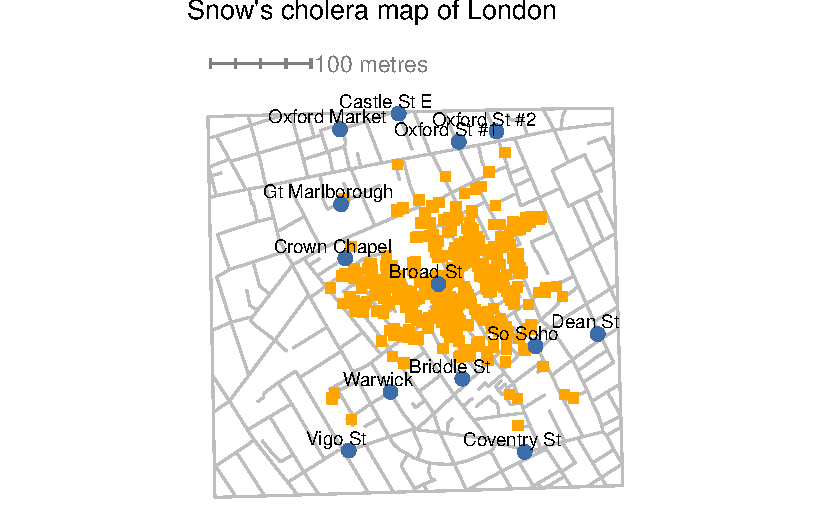
\includegraphics[width=1\textwidth,height=\textheight]{./05-Drawing-graphs_files/figure-pdf/fig-fig5-1-1.pdf} \hfill{}

\caption{\label{fig-fig5-1}A stylised redrawing of John Snow's original
cholera map. Each small orange square represents the location of a
cholera death and each blue circle shows the location of a water pump.
As the plot makes clear, the cholera outbreak is centred very closely on
the Broad St pump}

\end{figure}

\hypertarget{sec-Histograms}{%
\section{Histograms}\label{sec-Histograms}}

Let's begin with the humble \textbf{histogram}. Histograms are one of
the simplest and most useful ways of visualising data. They make most
sense when you have an interval or ratio scale variable (e.g., the
afl.margins data from \textbf{?@sec-Descriptive-statistics} and what you
want to do is get an overall impression of the variable. Most of you
probably know how histograms work, since they're so widely used, but for
the sake of completeness I'll describe them. All you do is divide up the
possible values into \textbf{bins} and then count the number of
observations that fall within each bin. This count is referred to as the
frequency or density of the bin and is displayed as a vertical bar. Ihe
AFL winning margins data there are 33 games in which the winning margin
was less than 10 points and it is this fact that is represented by the
height of the leftmost bar that we showed earlier in
\textbf{?@sec-Descriptive-statistics}, \textbf{?@fig-fig4-2}. With these
earlier graphs we used an advanced plotting package in R which, for now,
is beyond the capability of jamovi. But jamovi gets us close, and
drawing this histogram in jamovi is pretty straightforward. Open up the
`plots' options under `Exploration' - `Descriptives' and click the
`histogram' check box, as in Figure~\ref{fig-fig5-1}. jamovi defaults to
labelling the y-axis as `density' and the x-axis with the variable name.
The \textbf{bins} are selected automatically, and there is no scale, or
count, information on the y-axis unlike the previous
\textbf{?@fig-fig4-2}. But this does not matter too much because after
all what we are really interested in is our impression of the shape of
the distribution: is it normally distributed or is there a skew or
kurtosis? Our first impressions of these characteristics come from
drawing a \textbf{histogram}.

\begin{figure}

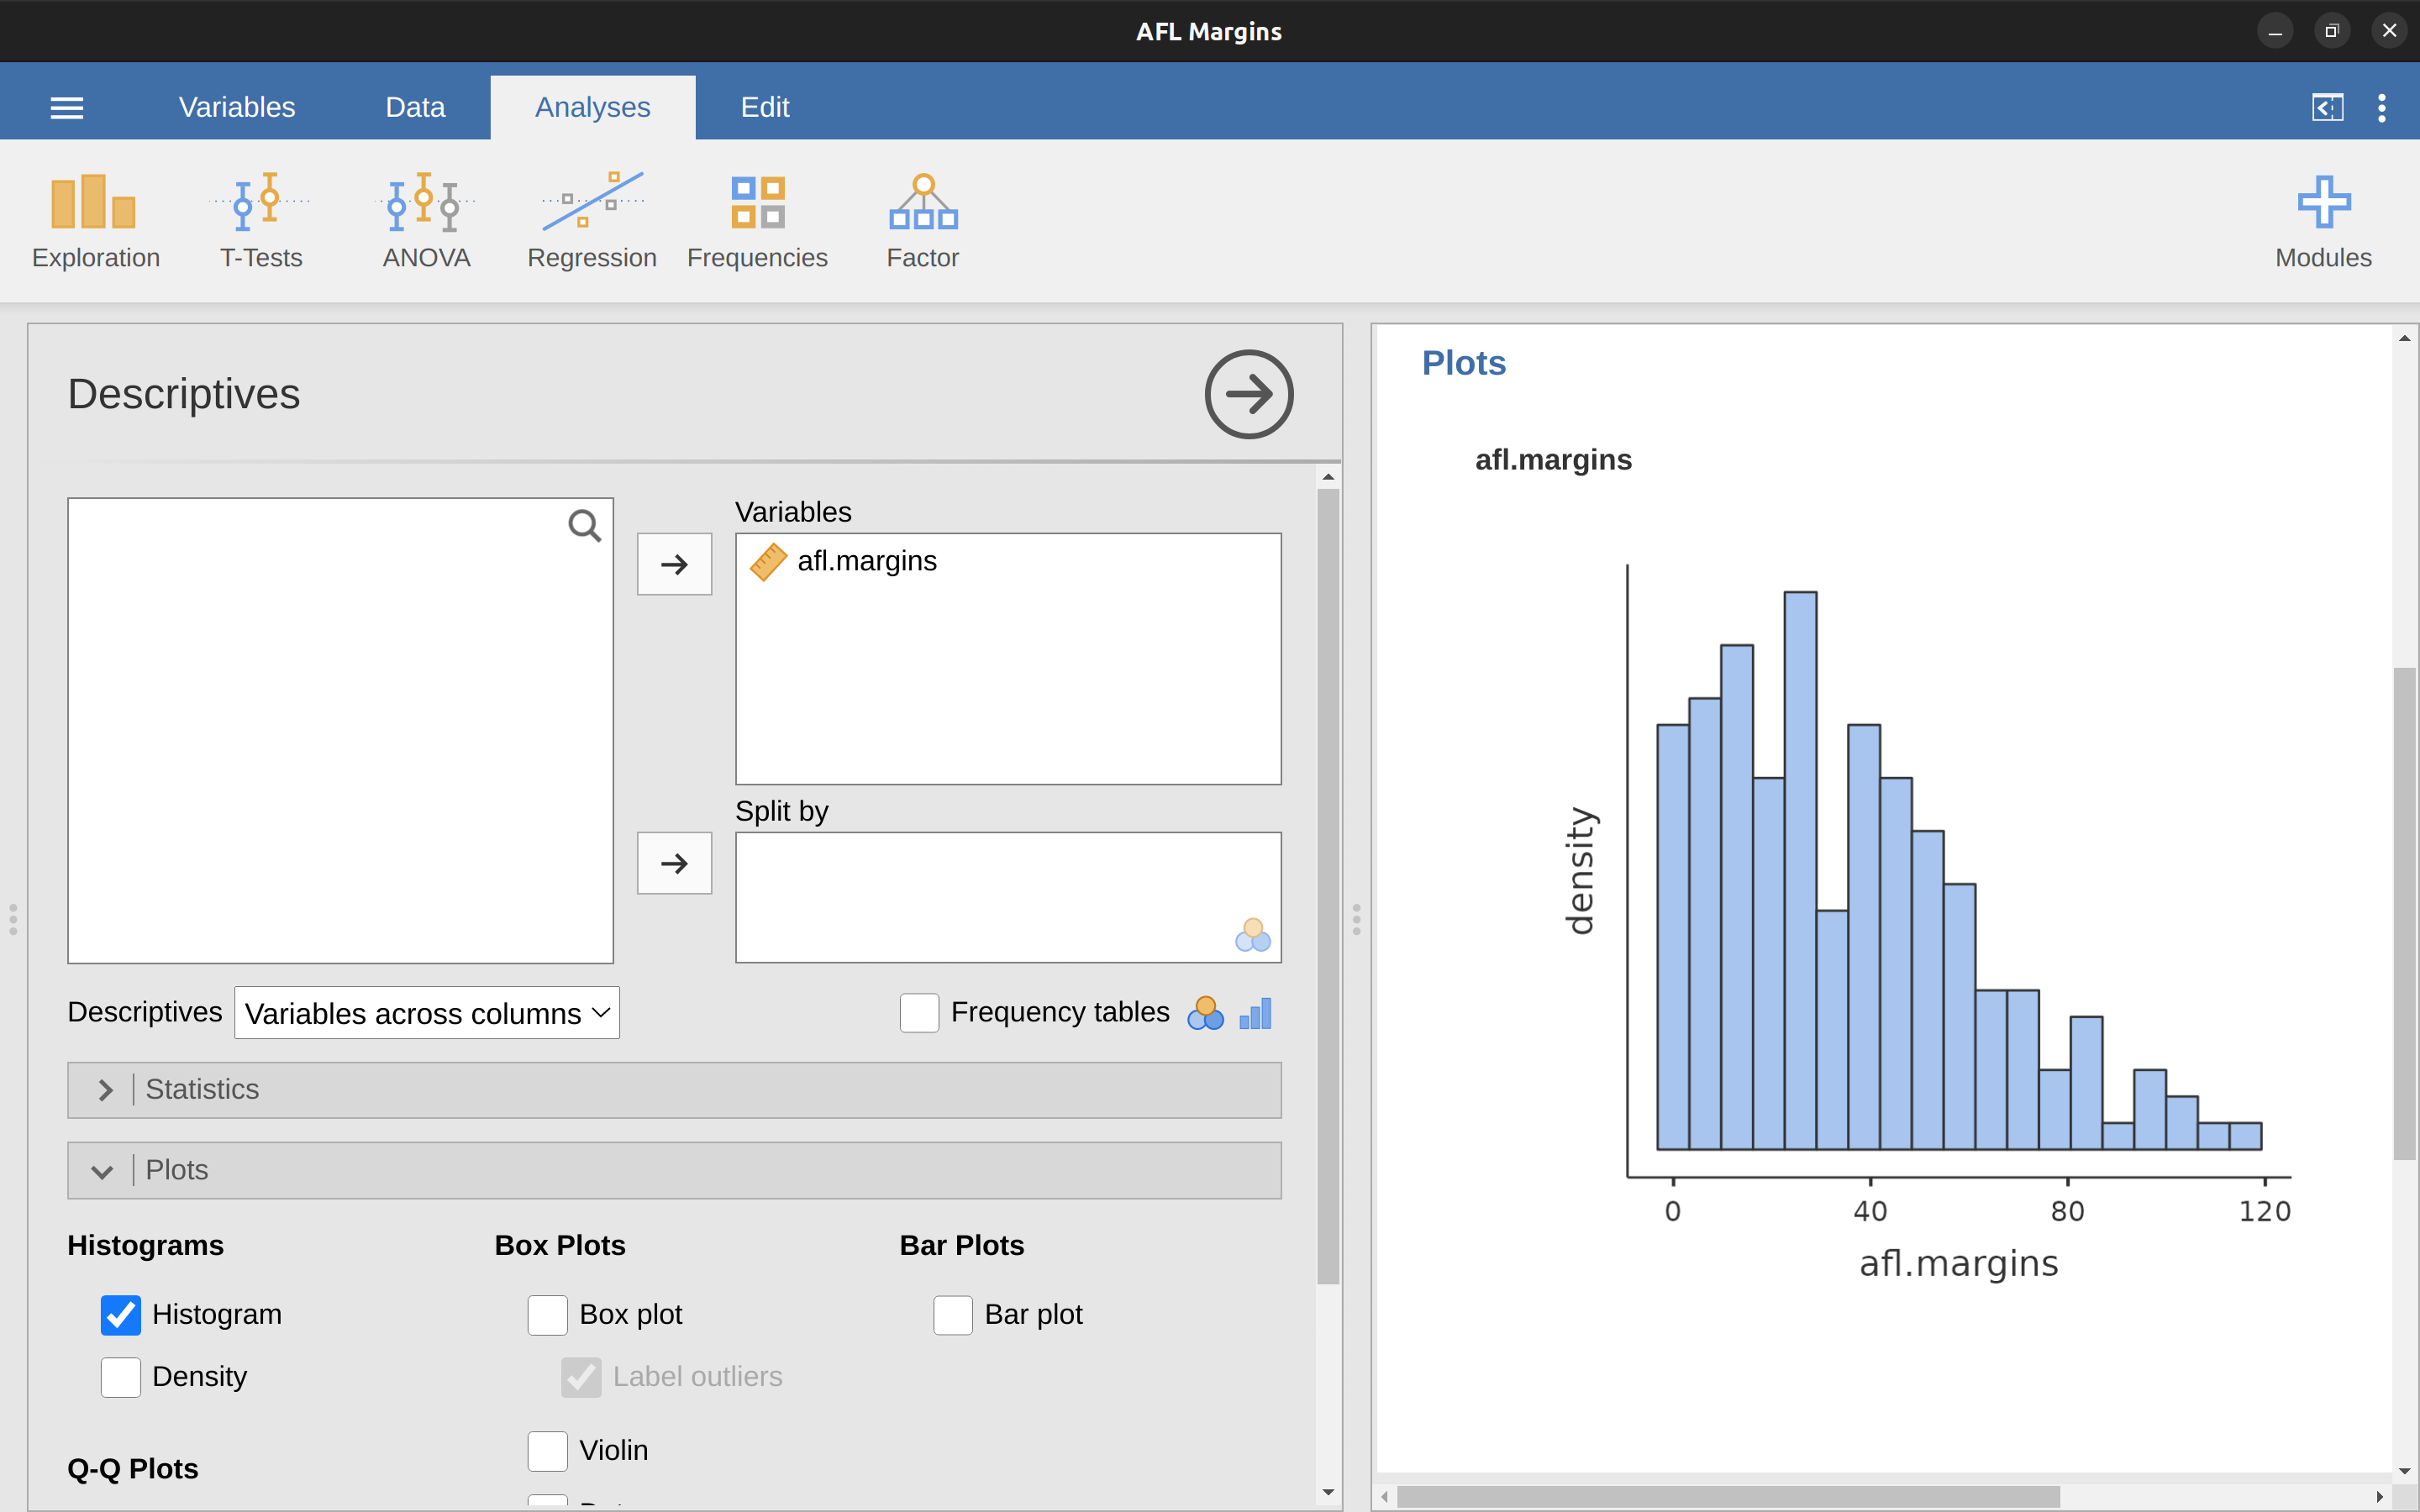
\includegraphics[width=0.8\textwidth,height=\textheight]{./images/fig5-2.png} \hfill{}

\caption{\label{fig-fig5-2}jamovi screen showing the histogram check
box}

\end{figure}

One additional feature that jamovi provides is the ability to plot a
`Density' curve. You can do this by clicking the `Density' check box
under the `Plots' options (and unchecking `Histogram'), and this gives
us the plot shown in Figure~\ref{fig-fig5-3}. A density plot visualises
the distribution of data over a continuous interval or time period. This
chart is a variation of a histogram that uses \textbf{kernel smoothing}
to plot values, allowing for smoother distributions by smoothing out the
noise. The peaks of a density plot help display where values are
concentrated over the interval. An advantage density plots have over
histograms is that they are better at determining the distribution shape
because they're not affected by the number of bins used (each bar used
in a typical histogram). A histogram comprising of only 4 bins wouldn't
produce a distinguishable enough shape of distribution as a 20-bin
histogram would. However, with density plots, this isn't an issue.

\begin{figure}

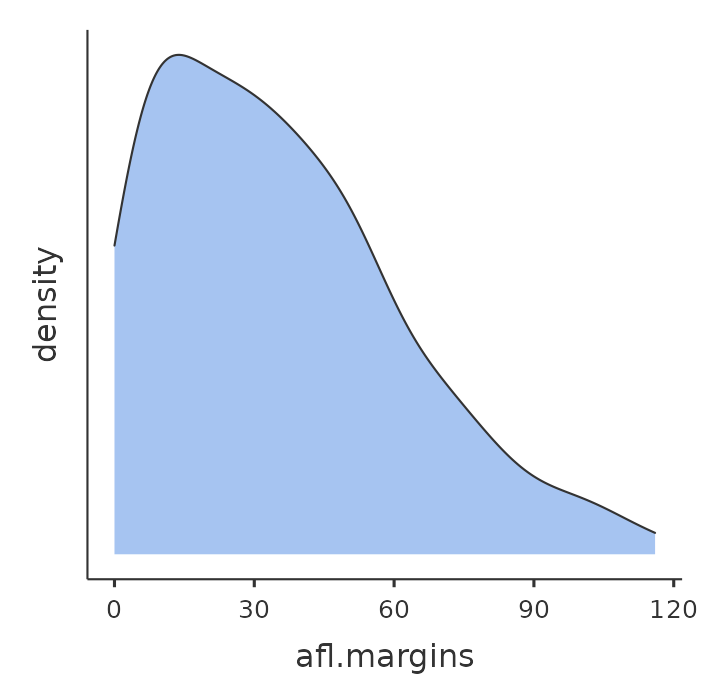
\includegraphics[width=0.8\textwidth,height=\textheight]{./images/fig5-3.png} \hfill{}

\caption{\label{fig-fig5-3}A density plot of the afl.margins variable
plotted in jamovi}

\end{figure}

Although this image would need a lot of cleaning up in order to make a
good presentation graphic (i.e., one you'd include in a report), it
nevertheless does a pretty good job of describing the data. In fact, the
big strength of a histogram or density plot is that (properly used) it
does show the entire spread of the data, so you can get a pretty good
sense about what it looks like. The downside to histograms is that they
aren't very compact. Unlike some of the other plots I'll talk about it's
hard to cram 20-30 histograms into a single image without overwhelming
the viewer. And of course, if your data are nominal scale then
histograms are useless.

\hypertarget{boxplots}{%
\section{Boxplots}\label{boxplots}}

Another alternative to histograms is a \textbf{boxplot}, sometimes
called a ``box and whiskers'' plot. Like histograms they're most suited
to interval or ratio scale data. The idea behind a boxplot is to provide
a simple visual depiction of the median, the interquartile range, and
the range of the data. And because they do so in a fairly compact way
boxplots have become a very popular statistical graphic, especially
during the exploratory stage of data analysis when you're trying to
understand the data yourself. Let's have a look at how they work, again
using the afl.margins data as our example.

\begin{figure}

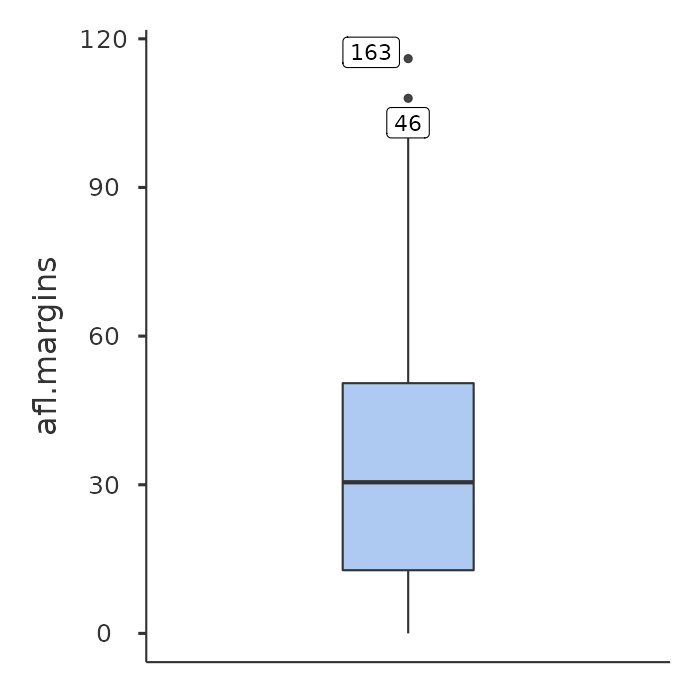
\includegraphics[width=0.8\textwidth,height=\textheight]{./images/fig5-4.png} \hfill{}

\caption{\label{fig-fig5-4}A box plot of the afl.margins variable
plotted in jamovi}

\end{figure}

The easiest way to describe what a boxplot looks like is just to draw
one. Click on the `Box plot' check box and you will get the plot shown
on the lower right of Figure~\ref{fig-fig5-4}. jamovi has drawn the most
basic boxplot possible. When you look at this plot this is how you
should interpret it: the thick line in the middle of the box is the
median; the box itself spans the range from the 25th percentile to the
75th percentile; and the ``whiskers'' go out to the most extreme data
point that doesn't exceed a certain bound. By default, this value is 1.5
times the interquartile range (IQR), calculated as 25th percentile -
(1.5*IQR) for the lower boundary, and 75th percentile + (1.5*IQR) for
the upper boundary. Any observation whose value falls outside this range
is plotted as a circle or dot instead of being covered by the whiskers,
and is commonly referred to as an \textbf{outlier}. For our AFL margins
data there are two observations that fall outside this range, and these
observations are plotted as dots (the upper boundary is 107, and looking
over the data column in the spreadsheet there are two observations with
values higher than this, 108 and 116, so these are the dots).

\hypertarget{violin-plots}{%
\subsection{Violin plots}\label{violin-plots}}

\begin{figure}

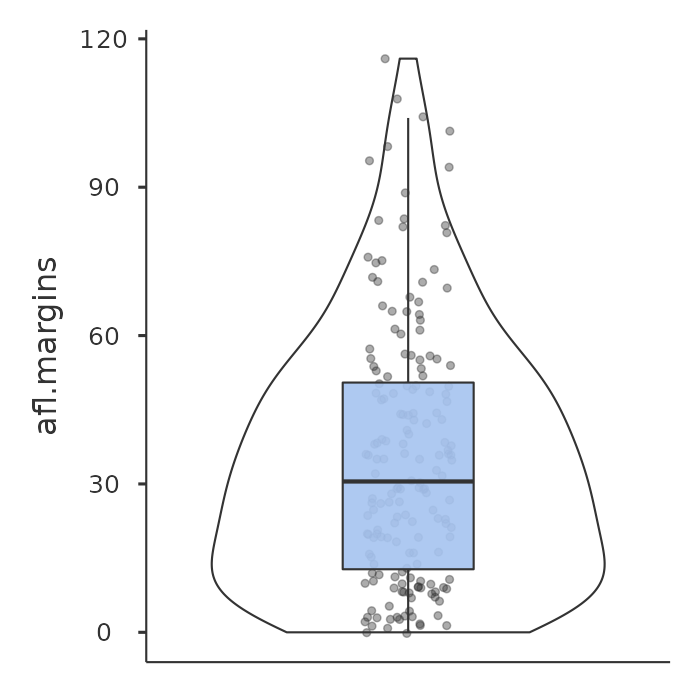
\includegraphics[width=0.8\textwidth,height=\textheight]{./images/fig5-5.png} \hfill{}

\caption{\label{fig-fig5-5}A violin plot of the afl.margins variable
plotted in jamovi, also showing a box plot and data points}

\end{figure}

A variation to the traditional box plot is the violin plot. Violin plots
are similar to box plots except that they also show the kernel
probability density of the data at different values. Typically, violin
plots will include a marker for the median of the data and a box
indicating the interquartile range, as in standard box plots. In jamovi
you can achieve this sort of functionality by checking both the `Violin'
and the `Box plot' check boxes. See Figure~\ref{fig-fig5-5}, which also
has the `Data' check box turned on to show the actual data points on the
plot. This does tend to make the graph a bit too busy though, in my
opinion. Clarity is simplicity, so in practice it might be better to
just use a simple box plot.

\hypertarget{drawing-multiple-boxplots}{%
\subsection{Drawing multiple boxplots}\label{drawing-multiple-boxplots}}

One last thing. What if you want to draw multiple boxplots at once?
Suppose, for instance, I wanted separate boxplots showing the AFL
margins not just for 2010 but for every year between 1987 and 2010. To
do that the first thing we'll have to do is find the data. These are
stored in the \textbf{aflmarginbyyear.csv} file. So let's load it into
jamovi and see what is in it. You will see that it is a pretty big data
set. It contains 4296 games and the variables that we're interested in.
What we want to do is have jamovi draw boxplots for the margin variable,
but plotted separately for each year. The way to do this is to move the
year variable across into the `Split by' box, as in
Figure~\ref{fig-fig5-6}.

\begin{figure}

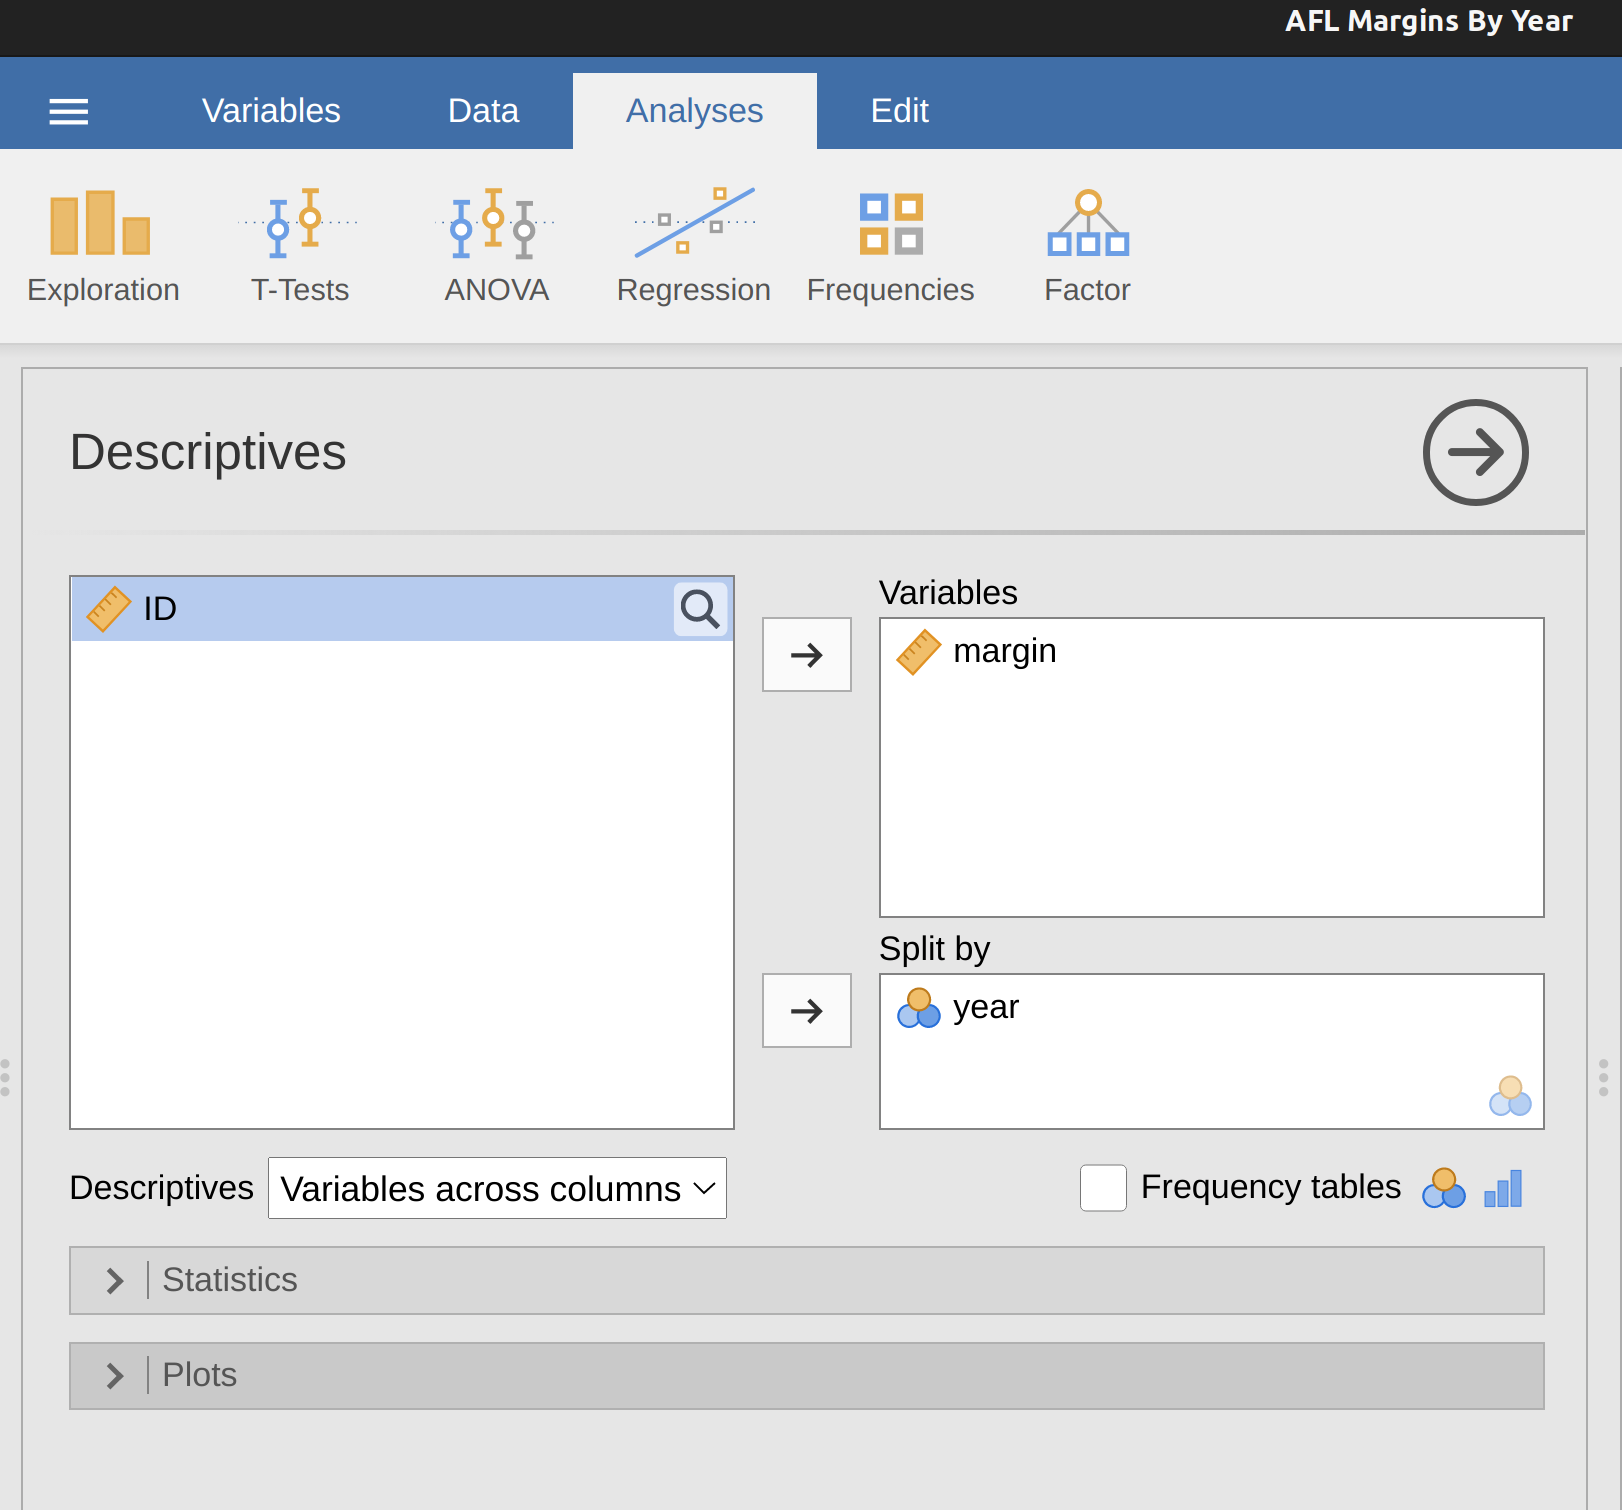
\includegraphics[width=0.8\textwidth,height=\textheight]{./images/fig5-6.png} \hfill{}

\caption{\label{fig-fig5-6}jamovi screen shot showing the `Split by'
window}

\end{figure}

The result is shown in Figure~\ref{fig-fig5-7}. This version of the box
plot, split by year, gives a sense of why it's sometimes useful to
choose box plots instead of histograms. It's possible to get a good
sense of what the data look like from year to year without getting
overwhelmed with too much detail. Now imagine what would have happened
if I'd tried to cram 24 histograms into this space: no chance at all
that the reader is going to learn anything useful.

\begin{figure}

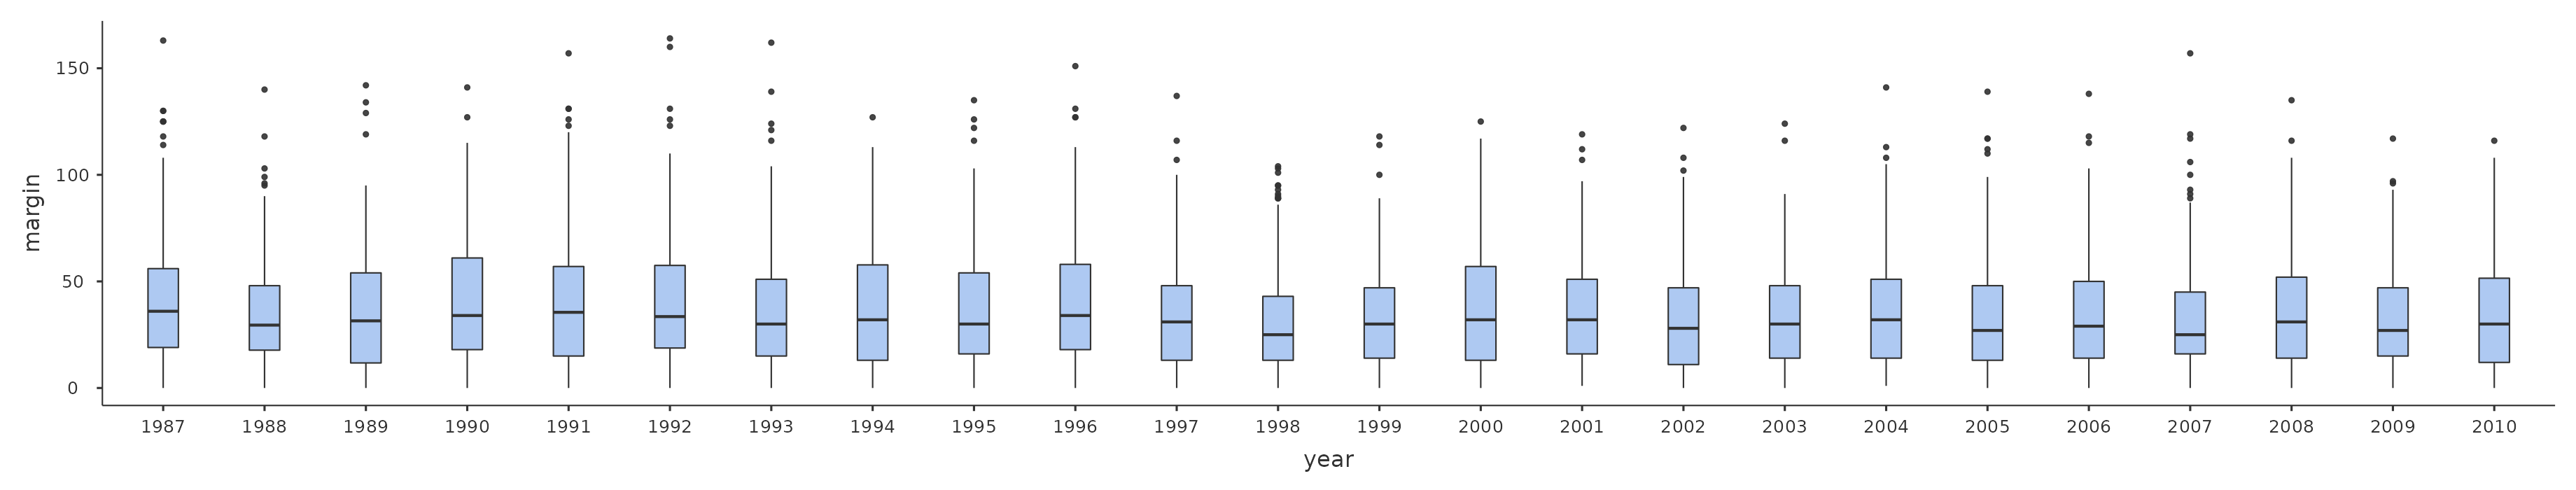
\includegraphics[width=0.8\textwidth,height=\textheight]{./images/fig5-7.png} \hfill{}

\caption{\label{fig-fig5-7}Multiple boxplots plotted in jamovi, for the
margin by year variables}

\end{figure}

\hypertarget{sec-Using-box-plots-to-detect-outliers}{%
\subsection{Using box plots to detect
outliers}\label{sec-Using-box-plots-to-detect-outliers}}

Because the boxplot automatically separates out those observations that
lie outside a certain range, depicting them with a dot in jamovi, people
often use them as an informal method for detecting \textbf{outliers}:
observations that are ``suspiciously'' distant from the rest of the
data. Here's an example. Suppose that I'd drawn the boxplot for the AFL
margins data and it came up looking like Figure~\ref{fig-fig5-8}. It's
pretty clear that something funny is going on with two of the
observations. Apparently, there were two games in which the margin was
over 300 points! That doesn't sound right to me. Now that I've become
suspicious it's time to look a bit more closely at the data. In jamovi
you can quickly find out which of these observations are suspicious and
then you can go back to the raw data to see if there has been a mistake
in data entry. One way to do this is to tell jamovi to label the
outliers, by checking the box next to the Box plot check box. This adds
a row number label next to the outlier in the boxplot, so you can go
look at that row and find the extreme value. Another, more flexible way,
is to set up a filter so that only those observations with values over a
certain threshold are included. In our example, the threshold is over
300, so that is the filter we will create. First, click on the `Filters'
button at the top of the jamovi window, and then type `margin
\textgreater{} 300' into the filter field, as in
Figure~\ref{fig-fig5-9}.

\begin{figure}

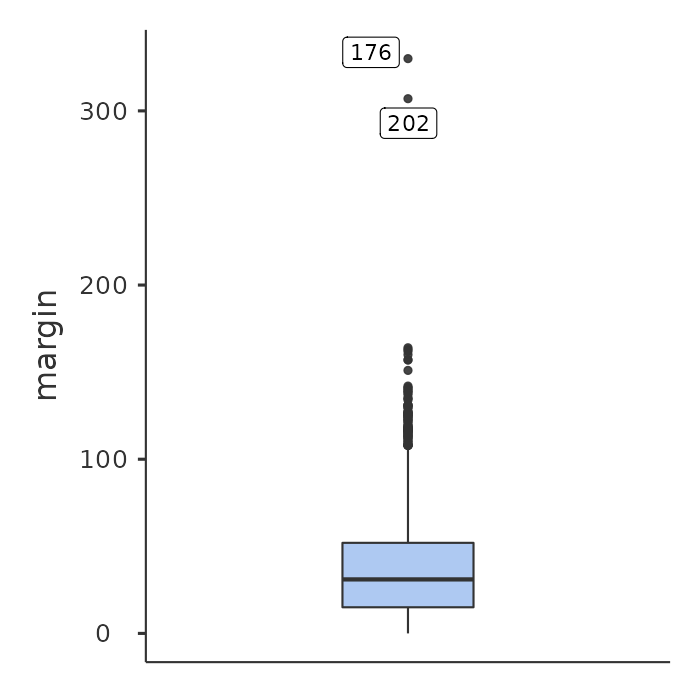
\includegraphics[width=0.8\textwidth,height=\textheight]{./images/fig5-8.png} \hfill{}

\caption{\label{fig-fig5-8}A boxplot showing two very suspicious
outliers!}

\end{figure}

This filter creates a new column in the spreadsheet view where only
those observations that pass the filter are included. One neat way to
quickly identify which observations these are is to tell jamovi to
produce a `Frequency table' (in the `Exploration' - `Descriptives'
window) for the ID variable (which must be a nominal variable otherwise
the Frequency table is not produced). In Figure~\ref{fig-fig5-10} you
can see that the ID values for the observations where the margin was
over 300 are 14 and 134. These are suspicious cases, or observations,
where you should go back to the original data source to find out what is
going on.

\begin{figure}

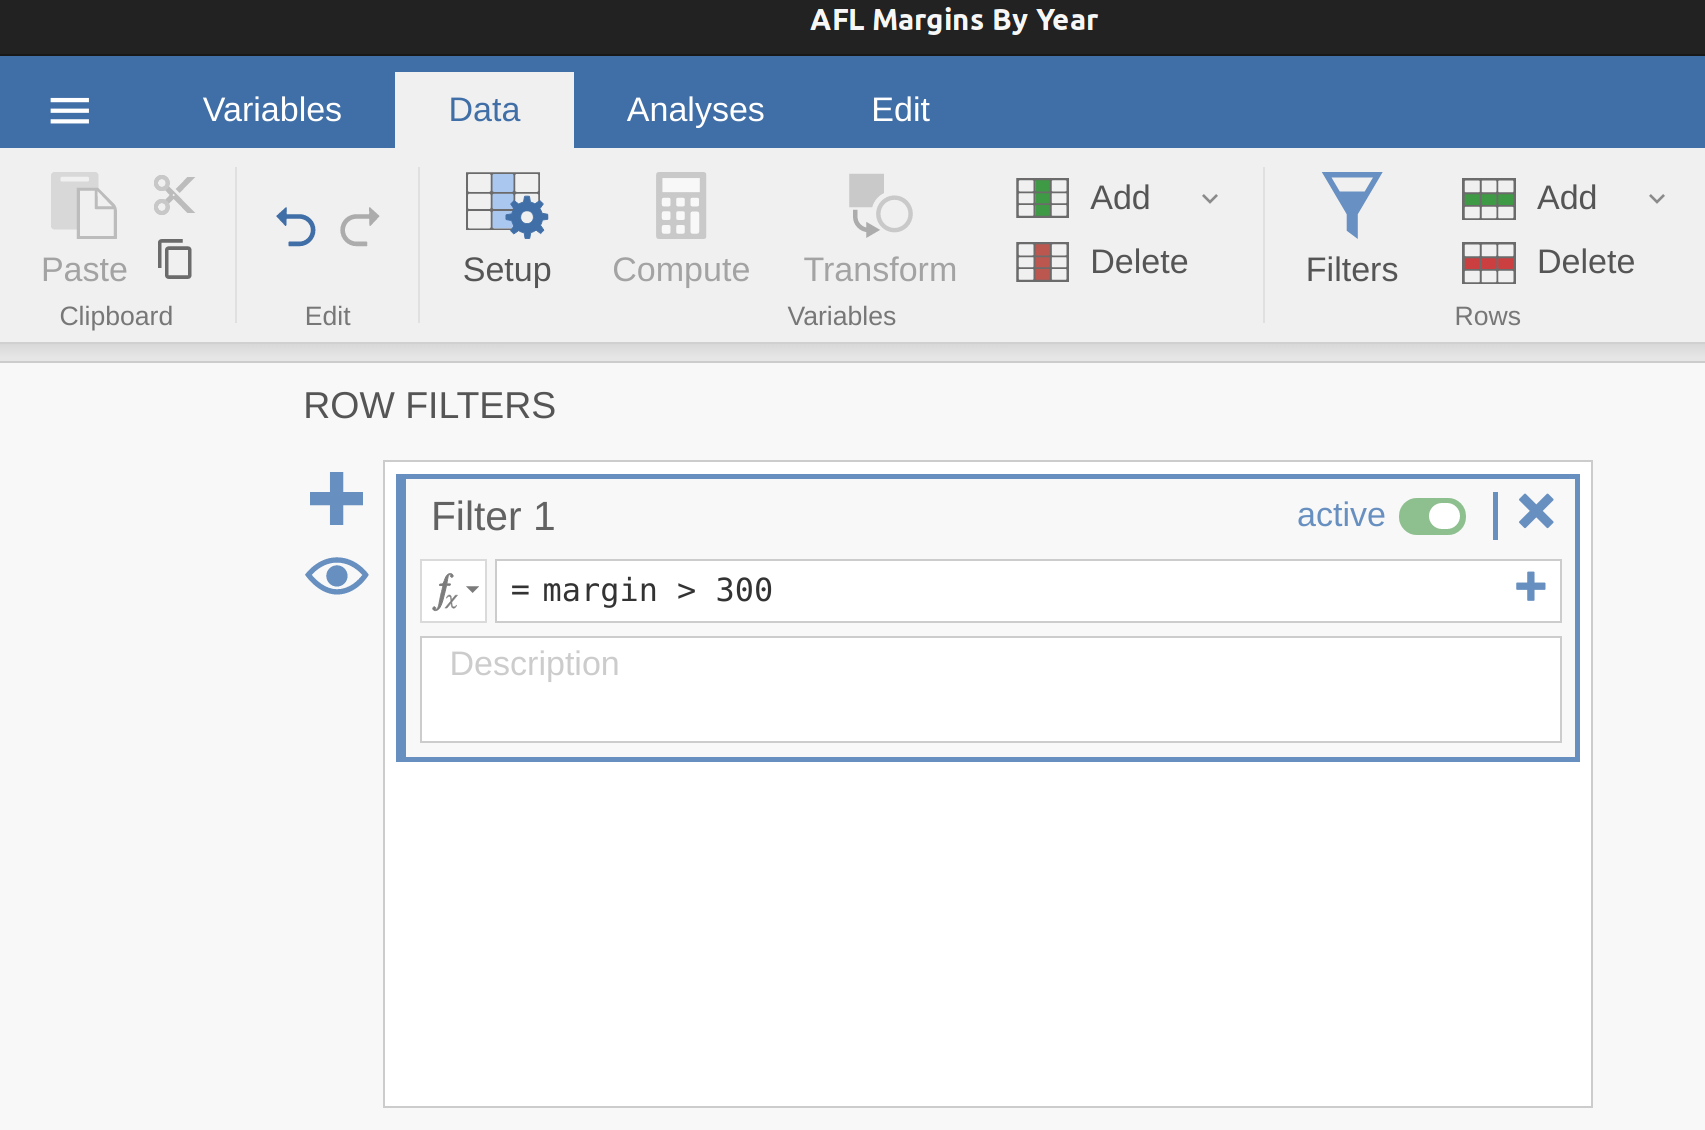
\includegraphics[width=0.8\textwidth,height=\textheight]{./images/fig5-9.png} \hfill{}

\caption{\label{fig-fig5-9}The jamovi filter screen}

\end{figure}

\begin{figure}

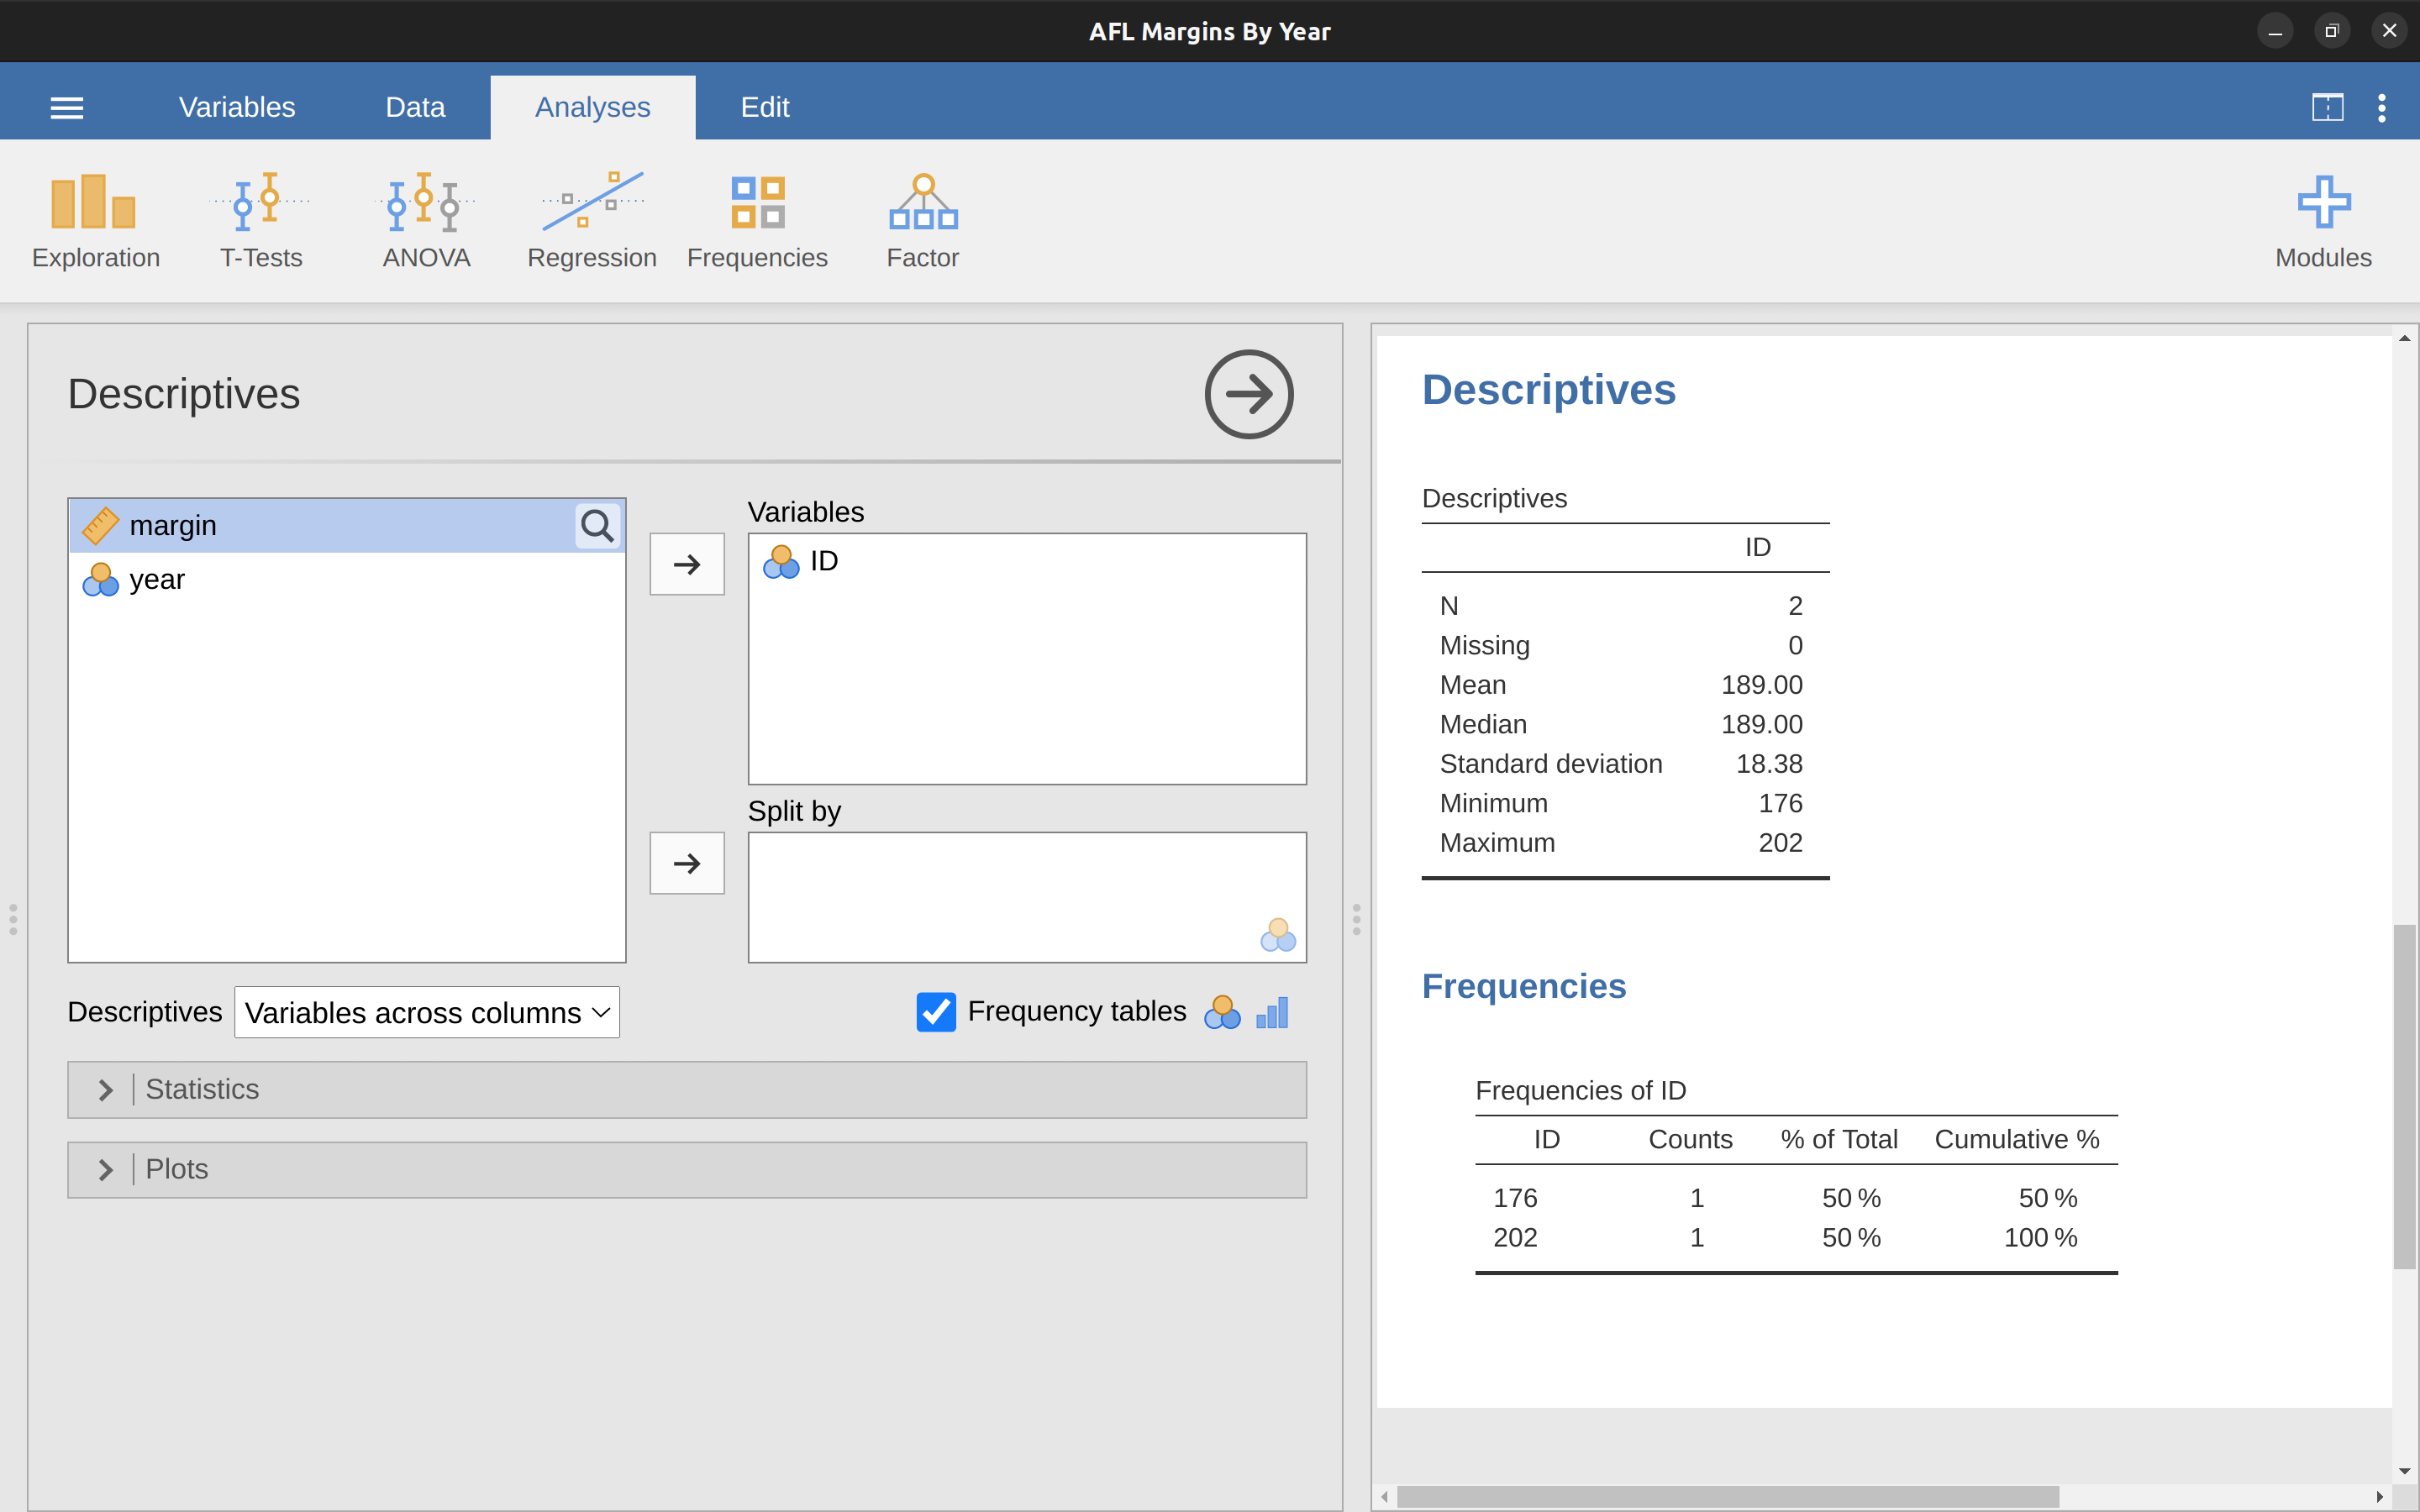
\includegraphics[width=0.8\textwidth,height=\textheight]{./images/fig5-10.png} \hfill{}

\caption{\label{fig-fig5-10}Frequency table for ID showing the ID
numbers for the two suspicious outliers, 14 and 134}

\end{figure}

Usually you find that someone has just typed in the wrong number. Whilst
this might seem like a silly example, I should stress that this kind of
thing actually happens a lot. Real world data sets are often riddled
with stupid errors, especially when someone had to type something into a
computer at some point. In fact, there's actually a name for this phase
of data analysis and in practice it can take up a huge chunk of our
time: data cleaning. It involves searching for typing mistakes
(``typos''), missing data and all sorts of other obnoxious errors in raw
data files.

For less extreme values, even if they are flagged in a a boxplot as
outliers, the decision about whether to include outliers or exclude them
in any analysis depends heavily on why you think the data look they way
they do and what you want to use the data for. You really need to
exercise good judgement here. If the outlier looks legitimate to you,
then keep it. In any case, I'll return to the topic again in
\textbf{?@sec-Model-checking} in
\textbf{?@sec-Correlation-and-linear-regression}.

\hypertarget{sec-Bar-graphs}{%
\section{Bar graphs}\label{sec-Bar-graphs}}

Another form of graph that you often want to plot is the \textbf{bar
graph}. Let's use the afl.finalists data set with the afl.finalists
variable that I introduced in \textbf{?@sec-Mode}. What I want to do is
draw a bar graph that displays the number of finals that each team has
played in over the time spanned by the afl.finalists data set. There are
lots of teams, but I am particularly interested in just four: Brisbane,
Carlton, Fremantle and Richmond. So the first step is to set up a filter
so just those four teams are included in the bar graph. This is
straightforward in jamovi and you can do it by using the `Filters'
function that we used previously. Open up the `Filters' screen and type
in the following:

afl.finalists \(==\) `Brisbane' or afl.finalists \(==\) `Carlton' or
afl.finalists \(==\) `Fremantle' or afl.finalists \(==\) `Richmond'
\footnote{jamovi uses the symbol ``\(==\)'' here to mean ``matches''.}

When you have done this you will see, in the `Data' view, that jamovi
has filtered out all values apart from those we have specified. Next,
open up the `Exploration' - `Descriptives' window and click on the `Bar
plot' check box (remember to move the `afl.finalists' variable across
into the `Variables' box so that jamovi knows which variable to use).
You should then get a bar graph, something like that shown in
Figure~\ref{fig-fig5-11}.

\begin{figure}

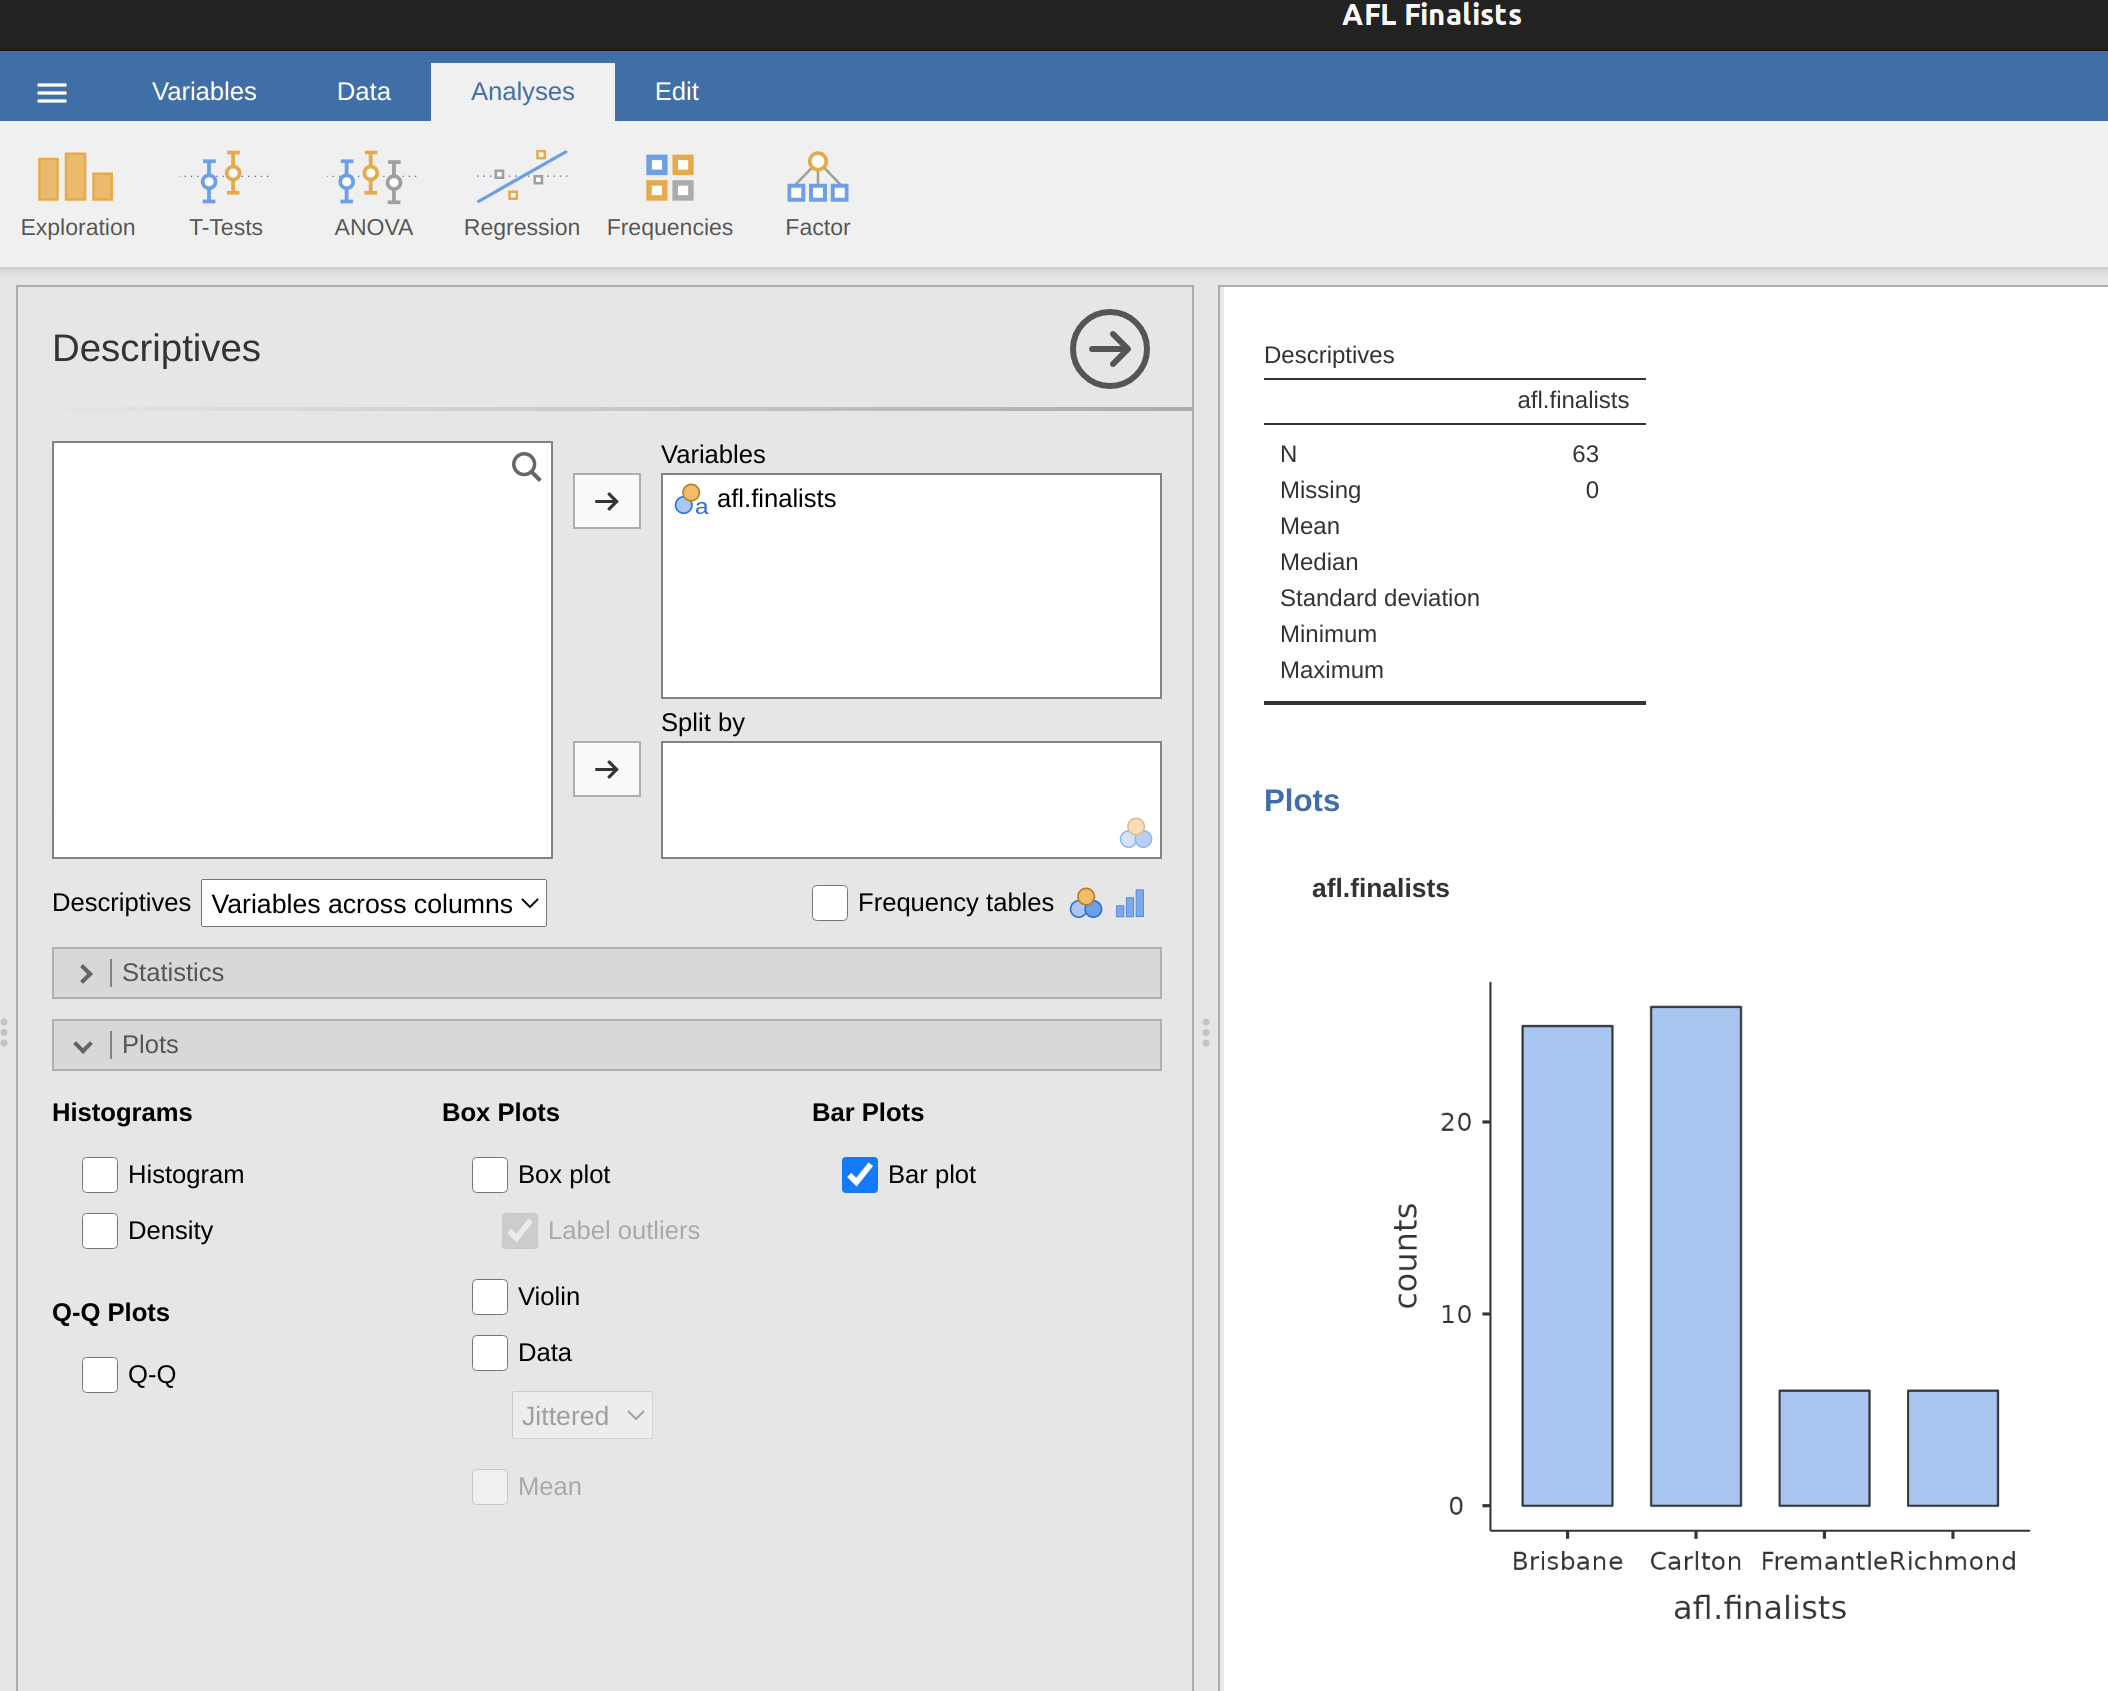
\includegraphics[width=0.8\textwidth,height=\textheight]{./images/fig5-11.png} \hfill{}

\caption{\label{fig-fig5-11}Filtering to include just four AFL teams,
and drawing a bar plot in jamovi}

\end{figure}

\hypertarget{saving-image-files-using-jamovi}{%
\section{Saving image files using
jamovi}\label{saving-image-files-using-jamovi}}

Hold on, you might be thinking. What's the good of being able to draw
pretty pictures in jamovi if I can't save them and send them to friends
to brag about how awesome my data is? How do I save the picture?
Simples. Just right click on the plot image and export it to a file,
either as `png', `eps', `svg' or `pdf'. These formats all produce nice
images that you can then send to your friends, or include in your
assignments or papers.

\hypertarget{summary-1}{%
\section{Summary}\label{summary-1}}

Perhaps I'm a simple minded person, but I love pictures. Every time I
write a new scientific paper one of the first things I do is sit down
and think about what the pictures will be. In my head an article is
really just a sequence of pictures linked together by a story. All the
rest of it is just window dressing. What I'm really trying to say here
is that the human visual system is a very powerful data analysis tool.
Give it the right kind of information and it will supply a human reader
with a massive amount of knowledge very quickly. Not for nothing do we
have the saying ``a picture is worth a thousand words''. With that in
mind, I think that this is one of the most important chapters in the
book. The topics covered were:

\begin{itemize}
\tightlist
\item
  \emph{Common plots}. Much of the chapter was focused on standard
  graphs that statisticians like to produce:
  \protect\hyperlink{sec-Histograms}{Histograms},
  \protect\hyperlink{boxplots}{Boxplots} and
  \protect\hyperlink{sec-Bar-graphs}{Bar graphs}
\item
  \protect\hyperlink{saving-image-files-using-jamovi}{Saving image files
  using jamovi}. Importantly, we also covered how to export your
  pictures.
\end{itemize}

One final thing to point out. Whilst jamovi produces some really neat
default graphics, editing the plots is currently not possible. For more
advanced graphics and plotting capability the packages available in R
are much more powerful. One of the most popular graphics systems is
provided by the ggplot2 package (see https://ggplot2.tidyverse.org/),
which is loosely based on ``The grammar of graphics'' (Wilkinson et al.,
2006). It's not for novices. You need to have a pretty good grasp of R
before you can start using it, and even then it takes a while to really
get the hang of it. But when you're ready it's worth taking the time to
teach yourself, because it's a much more powerful and cleaner system.

\begin{center}\rule{0.5\linewidth}{0.5pt}\end{center}

\part{Statistical theory}

\hypertarget{prelude}{%
\chapter*{Prelude}\label{prelude}}
\addcontentsline{toc}{chapter}{Prelude}

Part IV of the book is by far the most theoretical, focusing as it does
on the theory of statistical inference. Over the next three chapters my
goal is to give you an introduction to probability theory, sampling and
estimation in \textbf{?@sec-Estimating-unknown-quantities-from-a-sample}
and statistical hypothesis testing in \textbf{?@sec-Hypothesis-testing}.
Before we get started though, I want to say something about the big
picture. Statistical inference is primarily about learning from data.
The goal is no longer merely to describe our data but to use the data to
draw conclusions about the world. To motivate the discussion I want to
spend a bit of time talking about a philosophical puzzle known as the
riddle of induction, because it speaks to an issue that will pop up over
and over again throughout the book: statistical inference relies on
assumptions. This sounds like a bad thing. In everyday life people say
things like ``you should never make assumptions'', and psychology
classes often talk about assumptions and biases as bad things that we
should try to avoid. From bitter personal experience I have learned
never to say such things around philosophers!

\hypertarget{on-the-limits-of-logical-reasoning}{%
\section*{On the limits of logical
reasoning}\label{on-the-limits-of-logical-reasoning}}
\addcontentsline{toc}{section}{On the limits of logical reasoning}

\begin{quote}
\emph{The whole art of war consists in getting at what is on the other
side of the hill, or, in other words, in learning what we do not know
from what we do.}\\
- Arthur Wellesley, 1st Duke of Wellington
\end{quote}

I am told that quote above came about as a consequence of a carriage
ride across the countryside.\footnote{\href{\%0A\%20http://www.bartleby.com/344/400.html}{http://www.bartleby.com/344/400.html}}
He and his companion, J. W. Croker, were playing a guessing game, each
trying to predict what would be on the other side of each hill. In every
case it turned out that Wellesley was right and Croker was wrong. Many
years later when Wellesley was asked about the game he explained that
``the whole art of war consists in getting at what is on the other side
of the hill''. Indeed, war is not special in this respect. All of life
is a guessing game of one form or another, and getting by on a day to
day basis requires us to make good guesses. So let's play a guessing
game of our own.

Suppose you and I are observing the Wellesley-Croker competition and
after every three hills you and I have to predict who will win the next
one, Wellesley or Croker. Let's say that W refers to a Wellesley victory
and C refers to a Croker victory. After three hills, our data set looks
like this:

\(WWW\)

Our conversation goes like this:

\begin{quote}
you: Three in a row doesn't mean much. I suppose Wellesley might be
better at this than Croker, but it might just be luck. Still, I'm a bit
of a gambler. I'll bet on Wellesley.
\end{quote}

\begin{quote}
me: I agree that three in a row isn't informative and I see no reason to
prefer Wellesley's guesses over Croker's. I can't justify betting at
this stage. Sorry. No bet for me.
\end{quote}

Your gamble paid off: three more hills go by and Wellesley wins all
three. Going into the next round of our game the score is 1-0 in favour
of you and our data set looks like this: \(WWW\) \(WWW\) I've organised
the data into blocks of three so that you can see which batch
corresponds to the observations that we had available at each step in
our little side game. After seeing this new batch, our conversation
continues:

\begin{quote}
you: Six wins in a row for Duke Wellesley. This is starting to feel a
bit suspicious. I'm still not certain, but I reckon that he's going to
win the next one too.
\end{quote}

\begin{quote}
me: I guess I don't see that. Sure, I agree that Wellesley has won six
in a row, but I don't see any logical reason why that means he'll win
the seventh one. No bet. you: Do you really think so? Fair enough, but
my bet worked out last time and I'm okay with my choice.
\end{quote}

For a second time you were right, and for a second time I was wrong.
Wellesley wins the next three hills, extending his winning record
against Croker to 9-0. The data set available to us is now this: \(WWW\)
\(WWW\) \(WWW\) And our conversation goes like this:

\begin{quote}
you: Okay, this is pretty obvious. Wellesley is way better at this game.
We both agree he's going to win the next hill, right?
\end{quote}

\begin{quote}
me: Is there really any logical evidence for that? Before we started
this game, there were lots of possibilities for the first 10 outcomes,
and I had no idea which one to expect. \(WWW\) \(WWW\) \(WWW\) \(W\) was
one possibility, but so was \(WCC\) \(CWC\) \(WWC\) \(C\) and \(WWW\)
\(WWW\) \(WWW\) \(C\) or even \(CCC\) \(CCC\) \(CCC\) \(C\). Because I
had no idea what would happen so I'd have said they were all equally
likely. I assume you would have too, right? I mean, that's what it means
to say you have ``no idea'', isn't it?
\end{quote}

\begin{quote}
you: I suppose so.
\end{quote}

\begin{quote}
me: Well then, the observations we've made logically rule out all
possibilities except two: \(WWW\) \(WWW\) \(WWW\) \(C\) or \(WWW\)
\(WWW\) \(WWW\) \(W\). Both of these are perfectly consistent with the
evidence we've encountered so far, aren't they?
\end{quote}

\begin{quote}
you: Yes, of course they are. Where are you going with this? me: So
what's changed then? At the start of our game, you'd have agreed with me
that these are equally plausible and none of the evidence that we've
encountered has discriminated between these two possibilities.
Therefore, both of these possibilities remain equally plausible and I
see no logical reason to prefer one over the other. So yes, while I
agree with you that Wellesley's run of 9 wins in a row is remarkable, I
can't think of a good reason to think he'll win the 10th hill. No bet.
\end{quote}

\begin{quote}
you: I see your point, but I'm still willing to chance it. I'm betting
on Wellesley.
\end{quote}

Wellesley's winning streak continues for the next three hills. The score
in the Wellesley-Croker game is now 12-0, and the score in our game is
now 3-0. As we approach the fourth round of our game, our data set is
this: \(WWW\) \(WWW\) \(WWW\) \(WWW\) and the conversation continues:

\begin{quote}
you: Oh yeah! Three more wins for Wellesley and another victory for me.
Admit it, I was right about him! I guess we're both betting on Wellesley
this time around, right?
\end{quote}

\begin{quote}
me: I don't know what to think. I feel like we're in the same situation
we were in last round, and nothing much has changed. There are only two
legitimate possibilities for a sequence of 13 hills that haven't already
been ruled out, \(WWW\) \(WWW\) \(WWW\) \(WWW\) \(C\) and \(WWW\)
\(WWW\) \(WWW\) \(WWW\) \(W\). It's just like I said last time. If all
possible outcomes were equally sensible before the game started,
shouldn't these two be equally sensible now given that our observations
don't rule out either one? I agree that it feels like Wellesley is on an
amazing winning streak, but where's the logical evidence that the streak
will continue?
\end{quote}

\begin{quote}
you: I think you're being unreasonable. Why not take a look at our
scorecard, if you need evidence? You're the expert on statistics and
you've been using this fancy logical analysis, but the fact is you're
losing. I'm just relying on common sense and I'm winning. Maybe you
should switch strategies.
\end{quote}

\begin{quote}
me: Hmm, that is a good point and I don't want to lose the game, but I'm
afraid I don't see any logical evidence that your strategy is better
than mine. It seems to me that if there were someone else watching our
game, what they'd have observed is a run of three wins to you. Their
data would look like this: \(YYY\). Logically, I don't see that this is
any different to our first round of watching Wellesley and Croker. Three
wins to you doesn't seem like a lot of evidence, and I see no reason to
think that your strategy is working out any better than mine. If I
didn't think that \(WWW\) was good evidence then for Wellesley being
better than Croker at their game, surely I have no reason now to think
that YYY is good evidence that you're better at ours?
\end{quote}

\begin{quote}
you: Okay, now I think you're being a jerk.
\end{quote}

\begin{quote}
me: I don't see the logical evidence for that.
\end{quote}

\hypertarget{learning-without-making-assumptions-is-a-myth}{%
\section*{Learning without making assumptions is a
myth}\label{learning-without-making-assumptions-is-a-myth}}
\addcontentsline{toc}{section}{Learning without making assumptions is a
myth}

There are lots of different ways in which we could dissect this
dialogue, but since this is a statistics book pitched at psychologists
and not an introduction to the philosophy and psychology of reasoning,
I'll keep it brief. What I've described above is sometimes referred to
as the riddle of induction. It seems entirely reasonable to think that a
12-0 winning record by Wellesley is pretty strong evidence that he will
win the 13th game, but it is not easy to provide a proper logical
justification for this belief. On the contrary, despite the obviousness
of the answer, it's not actually possible to justify betting on
Wellesley without relying on some assumption that you don't have any
logical justification for.

The riddle of induction is most associated with the philosophical work
of David Hume and more recently Nelson Goodman, but you can find
examples of the problem popping up in fields as diverse as literature
(Lewis Carroll) and machine learning (the ``no free lunch'' theorem).
There really is something weird about trying to ``learn what we do not
know from what we do know''. The critical point is that assumptions and
biases are unavoidable if you want to learn anything about the world.
There is no escape from this, and it is just as true for statistical
inference as it is for human reasoning. In the dialogue I was taking aim
at your perfectly sensible inferences as a human being, but the common
sense reasoning that you relied on is no different to what a
statistician would have done. Your ``common sense'' half of the dialog
relied on an implicit assumption that there exists some difference in
skill between Wellesley and Croker, and what you were doing was trying
to work out what that difference in skill level would be. My ``logical
analysis'' rejects that assumption entirely. All I was willing to accept
is that there are sequences of wins and losses and that I did not know
which sequences would be observed. Throughout the dialogue I kept
insisting that all logically possible data sets were equally plausible
at the start of the Wellesely-Croker game, and the only way in which I
ever revised my beliefs was to eliminate those possibilities that were
factually inconsistent with the observations.

That sounds perfectly sensible on its own terms. In fact, it even sounds
like the hallmark of good deductive reasoning. Like Sherlock Holmes, my
approach was to rule out that which is impossible in the hope that what
would be left is the truth. Yet as we saw, ruling out the impossible
never led me to make a prediction. On its own terms everything I said in
my half of the dialogue was entirely correct. An inability to make any
predictions is the logical consequence of making ``no assumptions''. In
the end I lost our game because you did make some assumptions and those
assumptions turned out to be right. Skill is a real thing, and because
you believed in the existence of skill you were able to learn that
Wellesley had more of it than Croker. Had you relied on a less sensible
assumption to drive your learning you might not have won the game.

Ultimately there are two things you should take away from this. First,
as I've said, you cannot avoid making assumptions if you want to learn
anything from your data. But second, once you realise that assumptions
are necessary it becomes important to make sure you make the right ones!
A data analysis that relies on few assumptions is not necessarily better
than one that makes many assumptions, it all depends on whether those
assumptions are good ones for your data. As we go through the rest of
this book I'll often point out the assumptions that underpin a
particular statistical technique, and how you can check whether those
assumptions are sensible.

\begin{center}\rule{0.5\linewidth}{0.5pt}\end{center}

\hypertarget{sec-Introduction-to-probability}{%
\chapter{Introduction to
probability}\label{sec-Introduction-to-probability}}

\begin{quote}
\emph{{[}God{]} has afforded us only the twilight \ldots{} of
Probability.}\\
-- John Locke
\end{quote}

Up to this point in the book we've discussed some of the key ideas in
experimental design, and we've talked a little about how you can
summarise a data set. To a lot of people this is all there is to
statistics: collecting all the numbers, calculating averages, drawing
pictures, and putting them all in a report somewhere. Kind of like stamp
collecting but with numbers. However, statistics covers much more than
that. In fact, descriptive statistics is one of the smallest parts of
statistics and one of the least powerful. The bigger and more useful
part of statistics is that it provides information that lets you make
inferences about data.

Once you start thinking about statistics in these terms, that statistics
is there to help us draw inferences from data, you start seeing examples
of it everywhere. For instance, here's a tiny extract from a newspaper
article in the Sydney Morning Herald (30 Oct 2010):

\begin{quote}
``I have a tough job,'' the Premier said in response to a poll which
found her government is now the most unpopular Labor administration in
polling history, with a primary vote of just 23 per cent.
\end{quote}

This kind of remark is entirely unremarkable in the papers or in
everyday life, but let's have a think about what it entails. A polling
company has conducted a survey, usually a pretty big one because they
can afford it. I'm too lazy to track down the original survey so let's
just imagine that they called 1000 New South Wales (NSW) voters at
random, and 230 (23\%) of those claimed that they intended to vote for
the Australian Labor Party (ALP). For the 2010 Federal election the
Australian Electoral Commission reported 4,610,795 enrolled voters in
NSW, so the opinions of the remaining 4,609,795 voters (about 99.98\% of
voters) remain unknown to us. Even assuming that no-one lied to the
polling company the only thing we can say with 100\% confidence is that
the true ALP primary vote is somewhere between 230/4610795 (about
0.005\%) and 4610025/4610795 (about 99.83\%). So, on what basis is it
legitimate for the polling company, the newspaper, and the readership to
conclude that the ALP primary vote is only about 23\%?

The answer to the question is pretty obvious. If I call 1000 people at
random, and 230 of them say they intend to vote for the ALP, then it
seems very unlikely that these are the only 230 people out of the entire
voting public who actually intend to vote ALP. In other words, we assume
that the data collected by the polling company is pretty representative
of the population at large. But how representative? Would we be
surprised to discover that the true ALP primary vote is actually 24\%?
29\%? 37\%? At this point everyday intuition starts to break down a bit.
No-one would be surprised by 24\%, and everybody would be surprised by
37\%, but it's a bit hard to say whether 29\% is plausible. We need some
more powerful tools than just looking at the numbers and guessing.

\textbf{Inferential statistics} provides the tools that we need to
answer these sorts of questions, and since these kinds of questions lie
at the heart of the scientific enterprise, they take up the lions share
of every introductory course on statistics and research methods.
However, the theory of statistical inference is built on top of
\textbf{probability theory}. And it is to probability theory that we
must now turn. This discussion of probability theory is basically
background detail. There's not a lot of statistics per se in this
chapter, and you don't need to understand this material in as much depth
as the other chapters in this part of the book. Nevertheless, because
probability theory does underpin so much of statistics, it's worth
covering some of the basics.

\hypertarget{how-are-probability-and-statistics-different}{%
\section{How are probability and statistics
different?}\label{how-are-probability-and-statistics-different}}

Before we start talking about probability theory, it's helpful to spend
a moment thinking about the relationship between probability and
statistics. The two disciplines are closely related but they're not
identical. Probability theory is ``the doctrine of chances''. It's a
branch of mathematics that tells you how often different kinds of events
will happen. For example, all of these questions are things you can
answer using probability theory:

\begin{itemize}
\tightlist
\item
  What are the chances of a fair coin coming up heads 10 times in a row?
\item
  If I roll a six sided dice twice, how likely is it that I'll roll two
  sixes?
\item
  How likely is it that five cards drawn from a perfectly shuffled deck
  will all be hearts?
\item
  What are the chances that I'll win the lottery?
\end{itemize}

Notice that all of these questions have something in common. In each
case the ``truth of the world'' is known and my question relates to the
``what kind of events'' will happen. In the first question I know that
the coin is fair so there's a 50\% chance that any individual coin flip
will come up heads. In the second question I know that the chance of
rolling a 6 on a single die is 1 in 6. In the third question I know that
the deck is shuffled properly. And in the fourth question I know that
the lottery follows specific rules. You get the idea. The critical point
is that probabilistic questions start with a known \textbf{model} of the
world, and we use that model to do some calculations. The underlying
model can be quite simple. For instance, in the coin flipping example we
can write down the model like this:

\[P(head)=0.5\]

which you can read as ``the probability of heads is 0.5''. As we'll see
later, in the same way that percentages are numbers that range from 0\%
to 100\%, probabilities are just numbers that range from 0 to 1. When
using this probability model to answer the first question I don't
actually know exactly what's going to happen. Maybe I'll get 10 heads,
like the question says. But maybe I'll get three heads. That's the key
thing. In probability theory the model is known but the data are not.

So that's probability. What about statistics? Statistical questions work
the other way around. In statistics we do not know the truth about the
world. All we have is the data and it is from the data that we want to
learn the truth about the world. Statistical questions tend to look more
like these:

\begin{itemize}
\tightlist
\item
  If my friend flips a coin 10 times and gets 10 heads are they playing
  a trick on me?
\item
  If five cards off the top of the deck are all hearts how likely is it
  that the deck was shuffled?
\item
  If the lottery commissioner's spouse wins the lottery how likely is it
  that the lottery was rigged?
\end{itemize}

This time around the only thing we have are data. What I know is that I
saw my friend flip the coin 10 times and it came up heads every time.
And what I want to infer is whether or not I should conclude that what I
just saw was actually a fair coin being flipped 10 times in a row, or
whether I should suspect that my friend is playing a trick on me. The
data I have look like this:

H H H H H H H H H H H

and what I'm trying to do is work out which ``model of the world'' I
should put my trust in. If the coin is fair then the model I should
adopt is one that says that the probability of heads is 0.5, that is
P(heads) = 0.5. If the coin is not fair then I should conclude that the
probability of heads is not 0.5, which we would write as
\(P(heads)\ne{0.5}\). In other words, the statistical inference problem
is to figure out which of these probability models is right. Clearly,
the statistical question isn't the same as the probability question, but
they're deeply connected to one another. Because of this, a good
introduction to statistical theory will start with a discussion of what
probability is and how it works.

\hypertarget{what-does-probability-mean}{%
\section{What does probability mean?}\label{what-does-probability-mean}}

Let's start with the first of these questions. What is ``probability''?
It might seem surprising to you but while statisticians and
mathematicians (mostly) agree on what the rules of probability are,
there's much less of a consensus on what the word really means. It seems
weird because we're all very comfortable using words like ``chance'',
``likely'', ``possible'' and ``probable'', and it doesn't seem like it
should be a very difficult question to answer. But if you've ever had
that experience in real life you might walk away from the conversation
feeling like you didn't quite get it right, and that (like many everyday
concepts) it turns out that you don't really know what it's all about.

So I'll have a go at it. Let's suppose I want to bet on a soccer game
between two teams of robots, Arduino Arsenal and C Milan. After thinking
about it, I decide that there is an 80\% probability of Arduino Arsenal
winning. What do I mean by that? Here are three possibilities:

\begin{itemize}
\tightlist
\item
  They're robot teams so I can make them play over and over again, and
  if I did that Arduino Arsenal would win 8 out of every 10 games on
  average.
\item
  For any given game, I would agree that betting on this game is only
  ``fair'' if a \$1 bet on C Milan gives a \$5 payoff (i.e.~I get my \$1
  back plus a \$4 reward for being correct), as would a \$4 bet on
  Arduino Arsenal (i.e., my \$4 bet plus a \$1 reward).
\item
  My subjective ``belief'' or ``confidence'' in an Arduino Arsenal
  victory is four times as strong as my belief in a C Milan victory.
\end{itemize}

Each of these seems sensible. However, they're not identical and not
every statistician would endorse all of them. The reason is that there
are different statistical ideologies (yes, really!) and depending on
which one you subscribe to, you might say that some of those statements
are meaningless or irrelevant. In this section I give a brief
introduction the two main approaches that exist in the literature. These
are by no means the only approaches, but they're the two big ones.

\hypertarget{the-frequentist-view}{%
\subsection{The frequentist view}\label{the-frequentist-view}}

The first of the two major approaches to probability, and the more
dominant one in statistics, is referred to as the \textbf{frequentist
view} and it defines probability as a \textbf{long-run frequency}.
Suppose we were to try flipping a fair coin over and over again. By
definition this is a coin that has \(P(H) = 0.5\). What might we
observe? One possibility is that the first 20 flips might look like
this:

T,H,H,H,H,T,T,H,H,H,H,T,H,H,T,T,T,T,T,H

In this case 11 of these 20 coin flips (55\%) came up heads. Now suppose
that I'd been keeping a running tally of the number of heads (which I'll
call \(N_H\)) that I've seen, across the first N flips, and calculate
the proportion of heads \(\frac{N_H}{N}\) every time.
Table~\ref{tbl-tab7-1} shows what I'd get (I did literally flip coins to
produce this!):

\hypertarget{tbl-tab7-1}{}
 
  \providecommand{\huxb}[2]{\arrayrulecolor[RGB]{#1}\global\arrayrulewidth=#2pt}
  \providecommand{\huxvb}[2]{\color[RGB]{#1}\vrule width #2pt}
  \providecommand{\huxtpad}[1]{\rule{0pt}{#1}}
  \providecommand{\huxbpad}[1]{\rule[-#1]{0pt}{#1}}

\begin{table}[ht]
\caption{\label{tbl-tab7-1}Coin flips and proportion of heads }\tabularnewline

\begin{centerbox}
\begin{threeparttable}
\setlength{\tabcolsep}{0pt}
\begin{tabularx}{0.9\textwidth}{p{0.3\textwidth} p{0.3\textwidth} p{0.3\textwidth}}


\hhline{>{\huxb{0, 0, 0}{0.4}}->{\huxb{0, 0, 0}{0.4}}->{\huxb{0, 0, 0}{0.4}}-}
\arrayrulecolor{black}

\multicolumn{1}{!{\huxvb{0, 0, 0}{0}}p{0.3\textwidth}!{\huxvb{0, 0, 0}{0}}}{\cellcolor[RGB]{242, 242, 242}\hspace{0pt}\parbox[b]{0.3\textwidth-0pt-6pt}{\huxtpad{6pt + 1em}\centering \textbf{number of flips}\huxbpad{6pt}}} &
\multicolumn{1}{p{0.3\textwidth}!{\huxvb{0, 0, 0}{0}}}{\cellcolor[RGB]{242, 242, 242}\hspace{6pt}\parbox[b]{0.3\textwidth-6pt-6pt}{\huxtpad{6pt + 1em}\centering \textbf{number of heads}\huxbpad{6pt}}} &
\multicolumn{1}{p{0.3\textwidth}!{\huxvb{0, 0, 0}{0}}}{\cellcolor[RGB]{242, 242, 242}\hspace{6pt}\parbox[b]{0.3\textwidth-6pt-0pt}{\huxtpad{6pt + 1em}\centering \textbf{proportion}\huxbpad{6pt}}} \tabularnewline[-0.5pt]


\hhline{>{\huxb{0, 0, 0}{0.4}}->{\huxb{0, 0, 0}{0.4}}->{\huxb{0, 0, 0}{0.4}}-}
\arrayrulecolor{black}

\multicolumn{1}{!{\huxvb{0, 0, 0}{0}}p{0.3\textwidth}!{\huxvb{0, 0, 0}{0}}}{\hspace{0pt}\parbox[b]{0.3\textwidth-0pt-6pt}{\huxtpad{6pt + 1em}\centering 1\huxbpad{6pt}}} &
\multicolumn{1}{p{0.3\textwidth}!{\huxvb{0, 0, 0}{0}}}{\hspace{6pt}\parbox[b]{0.3\textwidth-6pt-6pt}{\huxtpad{6pt + 1em}\centering 0\huxbpad{6pt}}} &
\multicolumn{1}{p{0.3\textwidth}!{\huxvb{0, 0, 0}{0}}}{\hspace{6pt}\parbox[b]{0.3\textwidth-6pt-0pt}{\huxtpad{6pt + 1em}\centering 0.00\huxbpad{6pt}}} \tabularnewline[-0.5pt]


\hhline{}
\arrayrulecolor{black}

\multicolumn{1}{!{\huxvb{0, 0, 0}{0}}p{0.3\textwidth}!{\huxvb{0, 0, 0}{0}}}{\cellcolor[RGB]{242, 242, 242}\hspace{0pt}\parbox[b]{0.3\textwidth-0pt-6pt}{\huxtpad{6pt + 1em}\centering 2\huxbpad{6pt}}} &
\multicolumn{1}{p{0.3\textwidth}!{\huxvb{0, 0, 0}{0}}}{\cellcolor[RGB]{242, 242, 242}\hspace{6pt}\parbox[b]{0.3\textwidth-6pt-6pt}{\huxtpad{6pt + 1em}\centering 1\huxbpad{6pt}}} &
\multicolumn{1}{p{0.3\textwidth}!{\huxvb{0, 0, 0}{0}}}{\cellcolor[RGB]{242, 242, 242}\hspace{6pt}\parbox[b]{0.3\textwidth-6pt-0pt}{\huxtpad{6pt + 1em}\centering 0.50\huxbpad{6pt}}} \tabularnewline[-0.5pt]


\hhline{}
\arrayrulecolor{black}

\multicolumn{1}{!{\huxvb{0, 0, 0}{0}}p{0.3\textwidth}!{\huxvb{0, 0, 0}{0}}}{\hspace{0pt}\parbox[b]{0.3\textwidth-0pt-6pt}{\huxtpad{6pt + 1em}\centering 3\huxbpad{6pt}}} &
\multicolumn{1}{p{0.3\textwidth}!{\huxvb{0, 0, 0}{0}}}{\hspace{6pt}\parbox[b]{0.3\textwidth-6pt-6pt}{\huxtpad{6pt + 1em}\centering 2\huxbpad{6pt}}} &
\multicolumn{1}{p{0.3\textwidth}!{\huxvb{0, 0, 0}{0}}}{\hspace{6pt}\parbox[b]{0.3\textwidth-6pt-0pt}{\huxtpad{6pt + 1em}\centering 0.67\huxbpad{6pt}}} \tabularnewline[-0.5pt]


\hhline{}
\arrayrulecolor{black}

\multicolumn{1}{!{\huxvb{0, 0, 0}{0}}p{0.3\textwidth}!{\huxvb{0, 0, 0}{0}}}{\cellcolor[RGB]{242, 242, 242}\hspace{0pt}\parbox[b]{0.3\textwidth-0pt-6pt}{\huxtpad{6pt + 1em}\centering 4\huxbpad{6pt}}} &
\multicolumn{1}{p{0.3\textwidth}!{\huxvb{0, 0, 0}{0}}}{\cellcolor[RGB]{242, 242, 242}\hspace{6pt}\parbox[b]{0.3\textwidth-6pt-6pt}{\huxtpad{6pt + 1em}\centering 3\huxbpad{6pt}}} &
\multicolumn{1}{p{0.3\textwidth}!{\huxvb{0, 0, 0}{0}}}{\cellcolor[RGB]{242, 242, 242}\hspace{6pt}\parbox[b]{0.3\textwidth-6pt-0pt}{\huxtpad{6pt + 1em}\centering 0.75\huxbpad{6pt}}} \tabularnewline[-0.5pt]


\hhline{}
\arrayrulecolor{black}

\multicolumn{1}{!{\huxvb{0, 0, 0}{0}}p{0.3\textwidth}!{\huxvb{0, 0, 0}{0}}}{\hspace{0pt}\parbox[b]{0.3\textwidth-0pt-6pt}{\huxtpad{6pt + 1em}\centering 5\huxbpad{6pt}}} &
\multicolumn{1}{p{0.3\textwidth}!{\huxvb{0, 0, 0}{0}}}{\hspace{6pt}\parbox[b]{0.3\textwidth-6pt-6pt}{\huxtpad{6pt + 1em}\centering 4\huxbpad{6pt}}} &
\multicolumn{1}{p{0.3\textwidth}!{\huxvb{0, 0, 0}{0}}}{\hspace{6pt}\parbox[b]{0.3\textwidth-6pt-0pt}{\huxtpad{6pt + 1em}\centering 0.80\huxbpad{6pt}}} \tabularnewline[-0.5pt]


\hhline{}
\arrayrulecolor{black}

\multicolumn{1}{!{\huxvb{0, 0, 0}{0}}p{0.3\textwidth}!{\huxvb{0, 0, 0}{0}}}{\cellcolor[RGB]{242, 242, 242}\hspace{0pt}\parbox[b]{0.3\textwidth-0pt-6pt}{\huxtpad{6pt + 1em}\centering 6\huxbpad{6pt}}} &
\multicolumn{1}{p{0.3\textwidth}!{\huxvb{0, 0, 0}{0}}}{\cellcolor[RGB]{242, 242, 242}\hspace{6pt}\parbox[b]{0.3\textwidth-6pt-6pt}{\huxtpad{6pt + 1em}\centering 4\huxbpad{6pt}}} &
\multicolumn{1}{p{0.3\textwidth}!{\huxvb{0, 0, 0}{0}}}{\cellcolor[RGB]{242, 242, 242}\hspace{6pt}\parbox[b]{0.3\textwidth-6pt-0pt}{\huxtpad{6pt + 1em}\centering 0.67\huxbpad{6pt}}} \tabularnewline[-0.5pt]


\hhline{}
\arrayrulecolor{black}

\multicolumn{1}{!{\huxvb{0, 0, 0}{0}}p{0.3\textwidth}!{\huxvb{0, 0, 0}{0}}}{\hspace{0pt}\parbox[b]{0.3\textwidth-0pt-6pt}{\huxtpad{6pt + 1em}\centering 7\huxbpad{6pt}}} &
\multicolumn{1}{p{0.3\textwidth}!{\huxvb{0, 0, 0}{0}}}{\hspace{6pt}\parbox[b]{0.3\textwidth-6pt-6pt}{\huxtpad{6pt + 1em}\centering 4\huxbpad{6pt}}} &
\multicolumn{1}{p{0.3\textwidth}!{\huxvb{0, 0, 0}{0}}}{\hspace{6pt}\parbox[b]{0.3\textwidth-6pt-0pt}{\huxtpad{6pt + 1em}\centering 0.57\huxbpad{6pt}}} \tabularnewline[-0.5pt]


\hhline{}
\arrayrulecolor{black}

\multicolumn{1}{!{\huxvb{0, 0, 0}{0}}p{0.3\textwidth}!{\huxvb{0, 0, 0}{0}}}{\cellcolor[RGB]{242, 242, 242}\hspace{0pt}\parbox[b]{0.3\textwidth-0pt-6pt}{\huxtpad{6pt + 1em}\centering 8\huxbpad{6pt}}} &
\multicolumn{1}{p{0.3\textwidth}!{\huxvb{0, 0, 0}{0}}}{\cellcolor[RGB]{242, 242, 242}\hspace{6pt}\parbox[b]{0.3\textwidth-6pt-6pt}{\huxtpad{6pt + 1em}\centering 5\huxbpad{6pt}}} &
\multicolumn{1}{p{0.3\textwidth}!{\huxvb{0, 0, 0}{0}}}{\cellcolor[RGB]{242, 242, 242}\hspace{6pt}\parbox[b]{0.3\textwidth-6pt-0pt}{\huxtpad{6pt + 1em}\centering 0.63\huxbpad{6pt}}} \tabularnewline[-0.5pt]


\hhline{}
\arrayrulecolor{black}

\multicolumn{1}{!{\huxvb{0, 0, 0}{0}}p{0.3\textwidth}!{\huxvb{0, 0, 0}{0}}}{\hspace{0pt}\parbox[b]{0.3\textwidth-0pt-6pt}{\huxtpad{6pt + 1em}\centering 9\huxbpad{6pt}}} &
\multicolumn{1}{p{0.3\textwidth}!{\huxvb{0, 0, 0}{0}}}{\hspace{6pt}\parbox[b]{0.3\textwidth-6pt-6pt}{\huxtpad{6pt + 1em}\centering 6\huxbpad{6pt}}} &
\multicolumn{1}{p{0.3\textwidth}!{\huxvb{0, 0, 0}{0}}}{\hspace{6pt}\parbox[b]{0.3\textwidth-6pt-0pt}{\huxtpad{6pt + 1em}\centering 0.67\huxbpad{6pt}}} \tabularnewline[-0.5pt]


\hhline{}
\arrayrulecolor{black}

\multicolumn{1}{!{\huxvb{0, 0, 0}{0}}p{0.3\textwidth}!{\huxvb{0, 0, 0}{0}}}{\cellcolor[RGB]{242, 242, 242}\hspace{0pt}\parbox[b]{0.3\textwidth-0pt-6pt}{\huxtpad{6pt + 1em}\centering 10\huxbpad{6pt}}} &
\multicolumn{1}{p{0.3\textwidth}!{\huxvb{0, 0, 0}{0}}}{\cellcolor[RGB]{242, 242, 242}\hspace{6pt}\parbox[b]{0.3\textwidth-6pt-6pt}{\huxtpad{6pt + 1em}\centering 7\huxbpad{6pt}}} &
\multicolumn{1}{p{0.3\textwidth}!{\huxvb{0, 0, 0}{0}}}{\cellcolor[RGB]{242, 242, 242}\hspace{6pt}\parbox[b]{0.3\textwidth-6pt-0pt}{\huxtpad{6pt + 1em}\centering 0.70\huxbpad{6pt}}} \tabularnewline[-0.5pt]


\hhline{}
\arrayrulecolor{black}

\multicolumn{1}{!{\huxvb{0, 0, 0}{0}}p{0.3\textwidth}!{\huxvb{0, 0, 0}{0}}}{\hspace{0pt}\parbox[b]{0.3\textwidth-0pt-6pt}{\huxtpad{6pt + 1em}\centering 11\huxbpad{6pt}}} &
\multicolumn{1}{p{0.3\textwidth}!{\huxvb{0, 0, 0}{0}}}{\hspace{6pt}\parbox[b]{0.3\textwidth-6pt-6pt}{\huxtpad{6pt + 1em}\centering 8\huxbpad{6pt}}} &
\multicolumn{1}{p{0.3\textwidth}!{\huxvb{0, 0, 0}{0}}}{\hspace{6pt}\parbox[b]{0.3\textwidth-6pt-0pt}{\huxtpad{6pt + 1em}\centering 0.73\huxbpad{6pt}}} \tabularnewline[-0.5pt]


\hhline{}
\arrayrulecolor{black}

\multicolumn{1}{!{\huxvb{0, 0, 0}{0}}p{0.3\textwidth}!{\huxvb{0, 0, 0}{0}}}{\cellcolor[RGB]{242, 242, 242}\hspace{0pt}\parbox[b]{0.3\textwidth-0pt-6pt}{\huxtpad{6pt + 1em}\centering 12\huxbpad{6pt}}} &
\multicolumn{1}{p{0.3\textwidth}!{\huxvb{0, 0, 0}{0}}}{\cellcolor[RGB]{242, 242, 242}\hspace{6pt}\parbox[b]{0.3\textwidth-6pt-6pt}{\huxtpad{6pt + 1em}\centering 8\huxbpad{6pt}}} &
\multicolumn{1}{p{0.3\textwidth}!{\huxvb{0, 0, 0}{0}}}{\cellcolor[RGB]{242, 242, 242}\hspace{6pt}\parbox[b]{0.3\textwidth-6pt-0pt}{\huxtpad{6pt + 1em}\centering 0.67\huxbpad{6pt}}} \tabularnewline[-0.5pt]


\hhline{}
\arrayrulecolor{black}

\multicolumn{1}{!{\huxvb{0, 0, 0}{0}}p{0.3\textwidth}!{\huxvb{0, 0, 0}{0}}}{\hspace{0pt}\parbox[b]{0.3\textwidth-0pt-6pt}{\huxtpad{6pt + 1em}\centering 13\huxbpad{6pt}}} &
\multicolumn{1}{p{0.3\textwidth}!{\huxvb{0, 0, 0}{0}}}{\hspace{6pt}\parbox[b]{0.3\textwidth-6pt-6pt}{\huxtpad{6pt + 1em}\centering 9\huxbpad{6pt}}} &
\multicolumn{1}{p{0.3\textwidth}!{\huxvb{0, 0, 0}{0}}}{\hspace{6pt}\parbox[b]{0.3\textwidth-6pt-0pt}{\huxtpad{6pt + 1em}\centering 0.69\huxbpad{6pt}}} \tabularnewline[-0.5pt]


\hhline{}
\arrayrulecolor{black}

\multicolumn{1}{!{\huxvb{0, 0, 0}{0}}p{0.3\textwidth}!{\huxvb{0, 0, 0}{0}}}{\cellcolor[RGB]{242, 242, 242}\hspace{0pt}\parbox[b]{0.3\textwidth-0pt-6pt}{\huxtpad{6pt + 1em}\centering 14\huxbpad{6pt}}} &
\multicolumn{1}{p{0.3\textwidth}!{\huxvb{0, 0, 0}{0}}}{\cellcolor[RGB]{242, 242, 242}\hspace{6pt}\parbox[b]{0.3\textwidth-6pt-6pt}{\huxtpad{6pt + 1em}\centering 10\huxbpad{6pt}}} &
\multicolumn{1}{p{0.3\textwidth}!{\huxvb{0, 0, 0}{0}}}{\cellcolor[RGB]{242, 242, 242}\hspace{6pt}\parbox[b]{0.3\textwidth-6pt-0pt}{\huxtpad{6pt + 1em}\centering 0.71\huxbpad{6pt}}} \tabularnewline[-0.5pt]


\hhline{}
\arrayrulecolor{black}

\multicolumn{1}{!{\huxvb{0, 0, 0}{0}}p{0.3\textwidth}!{\huxvb{0, 0, 0}{0}}}{\hspace{0pt}\parbox[b]{0.3\textwidth-0pt-6pt}{\huxtpad{6pt + 1em}\centering 15\huxbpad{6pt}}} &
\multicolumn{1}{p{0.3\textwidth}!{\huxvb{0, 0, 0}{0}}}{\hspace{6pt}\parbox[b]{0.3\textwidth-6pt-6pt}{\huxtpad{6pt + 1em}\centering 10\huxbpad{6pt}}} &
\multicolumn{1}{p{0.3\textwidth}!{\huxvb{0, 0, 0}{0}}}{\hspace{6pt}\parbox[b]{0.3\textwidth-6pt-0pt}{\huxtpad{6pt + 1em}\centering 0.67\huxbpad{6pt}}} \tabularnewline[-0.5pt]


\hhline{}
\arrayrulecolor{black}

\multicolumn{1}{!{\huxvb{0, 0, 0}{0}}p{0.3\textwidth}!{\huxvb{0, 0, 0}{0}}}{\cellcolor[RGB]{242, 242, 242}\hspace{0pt}\parbox[b]{0.3\textwidth-0pt-6pt}{\huxtpad{6pt + 1em}\centering 16\huxbpad{6pt}}} &
\multicolumn{1}{p{0.3\textwidth}!{\huxvb{0, 0, 0}{0}}}{\cellcolor[RGB]{242, 242, 242}\hspace{6pt}\parbox[b]{0.3\textwidth-6pt-6pt}{\huxtpad{6pt + 1em}\centering 10\huxbpad{6pt}}} &
\multicolumn{1}{p{0.3\textwidth}!{\huxvb{0, 0, 0}{0}}}{\cellcolor[RGB]{242, 242, 242}\hspace{6pt}\parbox[b]{0.3\textwidth-6pt-0pt}{\huxtpad{6pt + 1em}\centering 0.63\huxbpad{6pt}}} \tabularnewline[-0.5pt]


\hhline{}
\arrayrulecolor{black}

\multicolumn{1}{!{\huxvb{0, 0, 0}{0}}p{0.3\textwidth}!{\huxvb{0, 0, 0}{0}}}{\hspace{0pt}\parbox[b]{0.3\textwidth-0pt-6pt}{\huxtpad{6pt + 1em}\centering 17\huxbpad{6pt}}} &
\multicolumn{1}{p{0.3\textwidth}!{\huxvb{0, 0, 0}{0}}}{\hspace{6pt}\parbox[b]{0.3\textwidth-6pt-6pt}{\huxtpad{6pt + 1em}\centering 10\huxbpad{6pt}}} &
\multicolumn{1}{p{0.3\textwidth}!{\huxvb{0, 0, 0}{0}}}{\hspace{6pt}\parbox[b]{0.3\textwidth-6pt-0pt}{\huxtpad{6pt + 1em}\centering 0.59\huxbpad{6pt}}} \tabularnewline[-0.5pt]


\hhline{}
\arrayrulecolor{black}

\multicolumn{1}{!{\huxvb{0, 0, 0}{0}}p{0.3\textwidth}!{\huxvb{0, 0, 0}{0}}}{\cellcolor[RGB]{242, 242, 242}\hspace{0pt}\parbox[b]{0.3\textwidth-0pt-6pt}{\huxtpad{6pt + 1em}\centering 18\huxbpad{6pt}}} &
\multicolumn{1}{p{0.3\textwidth}!{\huxvb{0, 0, 0}{0}}}{\cellcolor[RGB]{242, 242, 242}\hspace{6pt}\parbox[b]{0.3\textwidth-6pt-6pt}{\huxtpad{6pt + 1em}\centering 10\huxbpad{6pt}}} &
\multicolumn{1}{p{0.3\textwidth}!{\huxvb{0, 0, 0}{0}}}{\cellcolor[RGB]{242, 242, 242}\hspace{6pt}\parbox[b]{0.3\textwidth-6pt-0pt}{\huxtpad{6pt + 1em}\centering 0.56\huxbpad{6pt}}} \tabularnewline[-0.5pt]


\hhline{}
\arrayrulecolor{black}

\multicolumn{1}{!{\huxvb{0, 0, 0}{0}}p{0.3\textwidth}!{\huxvb{0, 0, 0}{0}}}{\hspace{0pt}\parbox[b]{0.3\textwidth-0pt-6pt}{\huxtpad{6pt + 1em}\centering 19\huxbpad{6pt}}} &
\multicolumn{1}{p{0.3\textwidth}!{\huxvb{0, 0, 0}{0}}}{\hspace{6pt}\parbox[b]{0.3\textwidth-6pt-6pt}{\huxtpad{6pt + 1em}\centering 10\huxbpad{6pt}}} &
\multicolumn{1}{p{0.3\textwidth}!{\huxvb{0, 0, 0}{0}}}{\hspace{6pt}\parbox[b]{0.3\textwidth-6pt-0pt}{\huxtpad{6pt + 1em}\centering 0.53\huxbpad{6pt}}} \tabularnewline[-0.5pt]


\hhline{}
\arrayrulecolor{black}

\multicolumn{1}{!{\huxvb{0, 0, 0}{0}}p{0.3\textwidth}!{\huxvb{0, 0, 0}{0}}}{\cellcolor[RGB]{242, 242, 242}\hspace{0pt}\parbox[b]{0.3\textwidth-0pt-6pt}{\huxtpad{6pt + 1em}\centering 20\huxbpad{6pt}}} &
\multicolumn{1}{p{0.3\textwidth}!{\huxvb{0, 0, 0}{0}}}{\cellcolor[RGB]{242, 242, 242}\hspace{6pt}\parbox[b]{0.3\textwidth-6pt-6pt}{\huxtpad{6pt + 1em}\centering 11\huxbpad{6pt}}} &
\multicolumn{1}{p{0.3\textwidth}!{\huxvb{0, 0, 0}{0}}}{\cellcolor[RGB]{242, 242, 242}\hspace{6pt}\parbox[b]{0.3\textwidth-6pt-0pt}{\huxtpad{6pt + 1em}\centering 0.55\huxbpad{6pt}}} \tabularnewline[-0.5pt]


\hhline{>{\huxb{0, 0, 0}{0.4}}->{\huxb{0, 0, 0}{0.4}}->{\huxb{0, 0, 0}{0.4}}-}
\arrayrulecolor{black}
\end{tabularx} 

\end{threeparttable}\par\end{centerbox}

\end{table}
 

Notice that at the start of the sequence the \emph{proportion} of heads
fluctuates wildly, starting at \(.00\) and rising as high as \(.80\).
Later on, one gets the impression that it dampens out a bit, with more
and more of the values actually being pretty close to the ``right''
answer of \(.50\). This is the frequentist definition of probability in
a nutshell. Flip a fair coin over and over again, and as N grows large
(approaches infinity, denoted \(N \rightarrow \infty\) ) the proportion
of heads will converge to 50\%. There are some subtle technicalities
that the mathematicians care about, but qualitatively speaking that's
how the frequentists define probability. Unfortunately, I don't have an
infinite number of coins or the infinite patience required to flip a
coin an infinite number of times. However, I do have a computer and
computers excel at mindless repetitive tasks. So I asked my computer to
simulate flipping a coin 1000 times and then drew a picture of what
happens to the proportion \(\frac{N_H}{N}\) as \(N\) increases.
Actually, I did it four times just to make sure it wasn't a fluke. The
results are shown in Figure~\ref{fig-fig7-1}. As you can see, the
proportion of observed heads eventually stops fluctuating and settles
down. When it does, the number at which it finally settles is the true
probability of heads.

The frequentist definition of probability has some desirable
characteristics. First, it is objective. The probability of an event is
\emph{necessarily} grounded in the world. The only way that probability
statements can make sense is if they refer to (a sequence of) events
that occur in the physical universe.\footnote{This doesn't mean that
  frequentists can't make hypothetical statements, of course. It's just
  that if you want to make a statement about probability then it must be
  possible to redescribe that statement in terms of a sequence of
  potentially observable events, together with the relative frequencies
  of different outcomes that appear within that sequence.} Secondly, it
is unambiguous. Any two people watching the same sequence of events
unfold, trying to calculate the probability of an event, must inevitably
come up with the same answer.

However, it also has undesirable characteristics. First, infinite
sequences don't exist in the physical world. Suppose you picked up a
coin from your pocket and started to flip it. Every time it lands it
impacts on the ground. Each impact wears the coin down a bit. Eventually
the coin will be destroyed. So, one might ask whether it really makes
sense to pretend that an ``infinite'' sequence of coin flips is even a
meaningful concept, or an objective one. We can't say that an ``infinite
sequence'' of events is a real thing in the physical universe, because
the physical universe doesn't allow infinite anything. More seriously,
the frequentist definition has a narrow scope. There are lots of things
out there that human beings are happy to assign probability to in
everyday language, but cannot (even in theory) be mapped onto a
hypothetical sequence of events. For instance, if a meteorologist comes
on TV and says ``the probability of rain in Adelaide on 2 November 2048
is 60\%'' we humans are happy to accept this. But it's not clear how to
define this in frequentist terms. There's only one city of Adelaide, and
only one 2 November 2048. There's no infinite sequence of events here,
just a one-off thing. Frequentist probability genuinely \emph{forbids}
us from making probability statements about a single event. From the
frequentist perspective it will either rain tomorrow or it will not.
There is no ``probability'' that attaches to a single non-repeatable
event. Now, it should be said that there are some very clever tricks
that frequentists can use to get around this. One possibility is that
what the meteorologist means is something like ``There is a category of
days for which I predict a 60\% chance of rain, and if we look only
across those days for which I make this prediction, then on 60\% of
those days it will actually rain''. It's very weird and
counter-intuitive to think of it this way, but you do see frequentists
do this sometimes. And it will come up later in this book (e.g.~in
\textbf{?@sec-Estimating-a-confidence-interval}).

\begin{figure}

\includegraphics[width=0.8\textwidth,height=\textheight]{./images/fig7-1.png} \hfill{}

\caption{\label{fig-fig7-1}An illustration of how frequentist
probability works. If you flip a fair coin over and over again the
proportion of heads that you've seen eventually settles down and
converges to the true probability of \(0.5\). Each panel shows four
different simulated experiments. In each case we pretend we flipped a
coin \(1000\) times and kept track of the proportion of flips that were
heads as we went along. Although none of these sequences actually ended
up with an exact value of \(.5\), if we'd extended the experiment for an
infinite number of coin flips they would have}

\end{figure}

\includegraphics{./07-Introduction-to-probability_files/figure-pdf/unnamed-chunk-4-1.pdf}

\hypertarget{the-bayesian-view}{%
\subsection{The Bayesian view}\label{the-bayesian-view}}

\textbf{The Bayesian view} of probability is often called the
subjectivist view, and although it has been a minority view among
statisticians it has been steadily gaining traction for the last several
decades. There are many flavours of Bayesianism, making it hard to say
exactly what ``the'' Bayesian view is. The most common way of thinking
about subjective probability is to define the probability of an event as
the \textbf{degree of belief} that an intelligent and rational agent
assigns to that truth of that event. From that perspective,
probabilities don't exist in the world but rather in the thoughts and
assumptions of people and other intelligent beings.

However, in order for this approach to work we need some way of
operationalising ``degree of belief''. One way that you can do this is
to formalise it in terms of ``rational gambling'', though there are many
other ways. Suppose that I believe that there's a 60\% probability of
rain tomorrow. If someone offers me a bet that if it rains tomorrow then
I win \$5, but if it doesn't rain I lose \$5. Clearly, from my
perspective, this is a pretty good bet. On the other hand, if I think
that the probability of rain is only 40\% then it's a bad bet to take.
So we can operationalise the notion of a ``subjective probability'' in
terms of what bets I'm willing to accept.

What are the advantages and disadvantages to the Bayesian approach? The
main advantage is that it allows you to assign probabilities to any
event you want to. You don't need to be limited to those events that are
repeatable. The main disadvantage (to many people) is that we can't be
purely objective. Specifying a probability requires us to specify an
entity that has the relevant degree of belief. This entity might be a
human, an alien, a robot, or even a statistician. But there has to be an
intelligent agent out there that believes in things. To many people this
is uncomfortable, it seems to make probability arbitrary. Whilst the
Bayesian approach requires that the agent in question be rational (i.e.,
obey the rules of probability), it does allow everyone to have their own
beliefs. I can believe the coin is fair and you don't have to, even
though we're both rational. The frequentist view doesn't allow any two
observers to attribute different probabilities to the same event. When
that happens then at least one of them must be wrong. The Bayesian view
does not prevent this from occurring. Two observers with different
background knowledge can legitimately hold different beliefs about the
same event. In short, where the frequentist view is sometimes considered
to be too narrow (forbids lots of things that that we want to assign
probabilities to), the Bayesian view is sometimes thought to be too
broad (allows too many differences between observers).

\hypertarget{whats-the-difference-and-who-is-right}{%
\subsection{What's the difference? And who is
right?}\label{whats-the-difference-and-who-is-right}}

Now that you've seen each of these two views independently it's useful
to make sure you can compare the two. Go back to the hypothetical robot
soccer game at the start of the section. What do you think a frequentist
and a Bayesian would say about these three statements? Which statement
would a frequentist say is the correct definition of probability? Which
one would a Bayesian opt for? Would some of these statements be
meaningless to a frequentist or a Bayesian? If you've understood the two
perspectives you should have some sense of how to answer those
questions.

Okay, assuming you understand the difference then you might be wondering
which of them is \emph{right}? Honestly, I don't know that there is a
right answer. As far as I can tell there's nothing mathematically
incorrect about the way frequentists think about sequences of events,
and there's nothing mathematically incorrect about the way that
Bayesians define the beliefs of a rational agent. In fact, when you dig
down into the details Bayesians and frequentists actually agree about a
lot of things. Many frequentist methods lead to decisions that Bayesians
agree a rational agent would make. Many Bayesian methods have very good
frequentist properties.

For the most part, I'm a pragmatist so I'll use any statistical method
that I trust. As it turns out, that makes me prefer Bayesian methods for
reasons I'll explain towards the end of the book. But I'm not
fundamentally opposed to frequentist methods. Not everyone is quite so
relaxed. For instance, consider Sir Ronald Fisher, one of the towering
figures of 20th century statistics and a vehement opponent to all things
Bayesian, whose paper on the mathematical foundations of statistics
referred to Bayesian probability as ``an impenetrable jungle {[}that{]}
arrests progress towards precision of statistical concepts'' (Fisher,
1922, p. 311). Or the psychologist Paul Meehl, who suggests that relying
on frequentist methods could turn you into ``a potent but sterile
intellectual rake who leaves in his merry path a long train of ravished
maidens but no viable scientific offspring'' (Meehl, 1967, p. 114). The
history of statistics, as you might gather, is not devoid of
entertainment.

In any case, whilst I personally prefer the Bayesian view, the majority
of statistical analyses are based on the frequentist approach. My
reasoning is pragmatic. The goal of this book is to cover roughly the
same territory as a typical undergraduate stats class in psychology, and
if you want to understand the statistical tools used by most
psychologists you'll need a good grasp of frequentist methods. I promise
you that this isn't wasted effort. Even if you end up wanting to switch
to the Bayesian perspective, you really should read through at least one
book on the ``orthodox'' frequentist view. Besides, I won't completely
ignore the Bayesian perspective. Every now and then I'll add some
commentary from a Bayesian point of view, and I'll revisit the topic in
more depth in \textbf{?@sec-Bayesian-statistics}.

\hypertarget{basic-probability-theory}{%
\section{Basic probability theory}\label{basic-probability-theory}}

Ideological arguments between Bayesians and frequentists
notwithstanding, it turns out that people mostly agree on the rules that
probabilities should obey. There are lots of different ways of arriving
at these rules. The most commonly used approach is based on the work of
Andrey Kolmogorov, one of the great Soviet mathematicians of the 20th
century. I won't go into a lot of detail, but I'll try to give you a bit
of a sense of how it works. And in order to do so I'm going to have to
talk about my trousers.

\hypertarget{introducing-probability-distributions}{%
\subsection{Introducing probability
distributions}\label{introducing-probability-distributions}}

One of the disturbing truths about my life is that I only own 5 pairs of
trousers. Three pairs of jeans, the bottom half of a suit, and a pair of
tracksuit pants. Even sadder, I've given them names: I call them
\(X_1\), \(X_2\), \(X_3\), \(X_4\) and \(X_5\). I really have, that's
why they call me Mister Imaginative. Now, on any given day, I pick out
exactly one of pair of trousers to wear. Not even I'm so stupid as to
try to wear two pairs of trousers, and thanks to years of training I
never go outside without wearing trousers anymore. If I were to describe
this situation using the language of probability theory, I would refer
to each pair of trousers (i.e., each \(X\)) as an elementary event. The
key characteristic of \textbf{elementary events} is that every time we
make an observation (e.g., every time I put on a pair of trousers) then
the outcome will be one and only one of these events. Like I said, these
days I always wear exactly one pair of trousers so my trousers satisfy
this constraint. Similarly, the set of all possible events is called a
\textbf{sample space}. Granted, some people would call it a
``wardrobe'', but that's because they're refusing to think about my
trousers in probabilistic terms. Sad.

Okay, now that we have a sample space (a wardrobe), which is built from
lots of possible elementary events (trousers), what we want to do is
assign a \textbf{probability} of one of these elementary events. For an
event \(X\), the probability of that event \(P(X)\) is a number that
lies between 0 and 1. The bigger the value of \(P(X)\), the more likely
the event is to occur. So, for example, if \(P(X) = 0\) it means the
event \(X\) is impossible (i.e., I never wear those trousers). On the
other hand, if \(P(X) = 1\) it means that event \(X\) is certain to
occur (i.e., I always wear those trousers). For probability values in
the middle it means that I sometimes wear those trousers. For instance,
if \(P(X) = 0.5\) it means that I wear those trousers half of the time.

At this point, we're almost done. The last thing we need to recognise is
that ``something always happens''. Every time I put on trousers, I
really do end up wearing trousers (crazy, right?). What this somewhat
trite statement means, in probabilistic terms, is that the probabilities
of the elementary events need to add up to 1. This is known as the
\textbf{law of total probability}, not that any of us really care. More
importantly, if these requirements are satisfied then what we have is a
\textbf{probability distribution}. For example, Table~\ref{tbl-tab7-2}
shows an example of a probability distribution.

\hypertarget{tbl-tab7-2}{}
 
  \providecommand{\huxb}[2]{\arrayrulecolor[RGB]{#1}\global\arrayrulewidth=#2pt}
  \providecommand{\huxvb}[2]{\color[RGB]{#1}\vrule width #2pt}
  \providecommand{\huxtpad}[1]{\rule{0pt}{#1}}
  \providecommand{\huxbpad}[1]{\rule[-#1]{0pt}{#1}}

\begin{table}[ht]
\caption{\label{tbl-tab7-2}A probability distribution for trouser wearing }\tabularnewline

\begin{centerbox}
\begin{threeparttable}
\setlength{\tabcolsep}{0pt}
\begin{tabularx}{0.9\textwidth}{p{0.3\textwidth} p{0.3\textwidth} p{0.3\textwidth}}


\hhline{>{\huxb{0, 0, 0}{0.4}}->{\huxb{0, 0, 0}{0.4}}->{\huxb{0, 0, 0}{0.4}}-}
\arrayrulecolor{black}

\multicolumn{1}{!{\huxvb{0, 0, 0}{0}}p{0.3\textwidth}!{\huxvb{0, 0, 0}{0}}}{\cellcolor[RGB]{242, 242, 242}\hspace{0pt}\parbox[b]{0.3\textwidth-0pt-6pt}{\huxtpad{6pt + 1em}\centering \textbf{Which trousers?}\huxbpad{6pt}}} &
\multicolumn{1}{p{0.3\textwidth}!{\huxvb{0, 0, 0}{0}}}{\cellcolor[RGB]{242, 242, 242}\hspace{6pt}\parbox[b]{0.3\textwidth-6pt-6pt}{\huxtpad{6pt + 1em}\centering \textbf{Label}\huxbpad{6pt}}} &
\multicolumn{1}{p{0.3\textwidth}!{\huxvb{0, 0, 0}{0}}}{\cellcolor[RGB]{242, 242, 242}\hspace{6pt}\parbox[b]{0.3\textwidth-6pt-0pt}{\huxtpad{6pt + 1em}\centering \textbf{Probability}\huxbpad{6pt}}} \tabularnewline[-0.5pt]


\hhline{>{\huxb{0, 0, 0}{0.4}}->{\huxb{0, 0, 0}{0.4}}->{\huxb{0, 0, 0}{0.4}}-}
\arrayrulecolor{black}

\multicolumn{1}{!{\huxvb{0, 0, 0}{0}}p{0.3\textwidth}!{\huxvb{0, 0, 0}{0}}}{\hspace{0pt}\parbox[b]{0.3\textwidth-0pt-6pt}{\huxtpad{6pt + 1em}\centering Blue jeans\huxbpad{6pt}}} &
\multicolumn{1}{p{0.3\textwidth}!{\huxvb{0, 0, 0}{0}}}{\hspace{6pt}\parbox[b]{0.3\textwidth-6pt-6pt}{\huxtpad{6pt + 1em}\centering \(X_1 \)\huxbpad{6pt}}} &
\multicolumn{1}{p{0.3\textwidth}!{\huxvb{0, 0, 0}{0}}}{\hspace{6pt}\parbox[b]{0.3\textwidth-6pt-0pt}{\huxtpad{6pt + 1em}\centering \(P(X_1)=.5 \)\huxbpad{6pt}}} \tabularnewline[-0.5pt]


\hhline{}
\arrayrulecolor{black}

\multicolumn{1}{!{\huxvb{0, 0, 0}{0}}p{0.3\textwidth}!{\huxvb{0, 0, 0}{0}}}{\cellcolor[RGB]{242, 242, 242}\hspace{0pt}\parbox[b]{0.3\textwidth-0pt-6pt}{\huxtpad{6pt + 1em}\centering Grey jeans\huxbpad{6pt}}} &
\multicolumn{1}{p{0.3\textwidth}!{\huxvb{0, 0, 0}{0}}}{\cellcolor[RGB]{242, 242, 242}\hspace{6pt}\parbox[b]{0.3\textwidth-6pt-6pt}{\huxtpad{6pt + 1em}\centering \(X_2 \)\huxbpad{6pt}}} &
\multicolumn{1}{p{0.3\textwidth}!{\huxvb{0, 0, 0}{0}}}{\cellcolor[RGB]{242, 242, 242}\hspace{6pt}\parbox[b]{0.3\textwidth-6pt-0pt}{\huxtpad{6pt + 1em}\centering \(P(X_2)=.3 \)\huxbpad{6pt}}} \tabularnewline[-0.5pt]


\hhline{}
\arrayrulecolor{black}

\multicolumn{1}{!{\huxvb{0, 0, 0}{0}}p{0.3\textwidth}!{\huxvb{0, 0, 0}{0}}}{\hspace{0pt}\parbox[b]{0.3\textwidth-0pt-6pt}{\huxtpad{6pt + 1em}\centering Black jeans\huxbpad{6pt}}} &
\multicolumn{1}{p{0.3\textwidth}!{\huxvb{0, 0, 0}{0}}}{\hspace{6pt}\parbox[b]{0.3\textwidth-6pt-6pt}{\huxtpad{6pt + 1em}\centering \(X_3 \)\huxbpad{6pt}}} &
\multicolumn{1}{p{0.3\textwidth}!{\huxvb{0, 0, 0}{0}}}{\hspace{6pt}\parbox[b]{0.3\textwidth-6pt-0pt}{\huxtpad{6pt + 1em}\centering \(P(X_3)=.1 \)\huxbpad{6pt}}} \tabularnewline[-0.5pt]


\hhline{}
\arrayrulecolor{black}

\multicolumn{1}{!{\huxvb{0, 0, 0}{0}}p{0.3\textwidth}!{\huxvb{0, 0, 0}{0}}}{\cellcolor[RGB]{242, 242, 242}\hspace{0pt}\parbox[b]{0.3\textwidth-0pt-6pt}{\huxtpad{6pt + 1em}\centering Black suit\huxbpad{6pt}}} &
\multicolumn{1}{p{0.3\textwidth}!{\huxvb{0, 0, 0}{0}}}{\cellcolor[RGB]{242, 242, 242}\hspace{6pt}\parbox[b]{0.3\textwidth-6pt-6pt}{\huxtpad{6pt + 1em}\centering \(X_4 \)\huxbpad{6pt}}} &
\multicolumn{1}{p{0.3\textwidth}!{\huxvb{0, 0, 0}{0}}}{\cellcolor[RGB]{242, 242, 242}\hspace{6pt}\parbox[b]{0.3\textwidth-6pt-0pt}{\huxtpad{6pt + 1em}\centering \(P(X_4)=0 \)\huxbpad{6pt}}} \tabularnewline[-0.5pt]


\hhline{}
\arrayrulecolor{black}

\multicolumn{1}{!{\huxvb{0, 0, 0}{0}}p{0.3\textwidth}!{\huxvb{0, 0, 0}{0}}}{\hspace{0pt}\parbox[b]{0.3\textwidth-0pt-6pt}{\huxtpad{6pt + 1em}\centering Blue tracksuit\huxbpad{6pt}}} &
\multicolumn{1}{p{0.3\textwidth}!{\huxvb{0, 0, 0}{0}}}{\hspace{6pt}\parbox[b]{0.3\textwidth-6pt-6pt}{\huxtpad{6pt + 1em}\centering \(X_5 \)\huxbpad{6pt}}} &
\multicolumn{1}{p{0.3\textwidth}!{\huxvb{0, 0, 0}{0}}}{\hspace{6pt}\parbox[b]{0.3\textwidth-6pt-0pt}{\huxtpad{6pt + 1em}\centering \(P(X_5)=.1 \)\huxbpad{6pt}}} \tabularnewline[-0.5pt]


\hhline{>{\huxb{0, 0, 0}{0.4}}->{\huxb{0, 0, 0}{0.4}}->{\huxb{0, 0, 0}{0.4}}-}
\arrayrulecolor{black}
\end{tabularx} 

\end{threeparttable}\par\end{centerbox}

\end{table}
 

Each of the events has a probability that lies between 0 and 1, and if
we add up the probability of all events they sum to 1. Awesome. We can
even draw a nice bar graph (see Section~\ref{sec-Bar-graphs}) to
visualise this distribution, as shown in Figure~\ref{fig-fig7-2}. And,
at this point, we've all achieved something. You've learned what a
probability distribution is, and I've finally managed to find a way to
create a graph that focuses entirely on my trousers. Everyone wins! The
only other thing that I need to point out is that probability theory
allows you to talk about \textbf{non elementary events} as well as
elementary ones. The easiest way to illustrate the concept is with an
example. In the trousers example it's perfectly legitimate to refer to
the probability that I wear jeans. In this scenario, the ``Dani wears
jeans'' event is said to have happened as long as the elementary event
that actually did occur is one of the appropriate ones. In this case
``blue jeans'', ``black jeans'' or ``grey jeans''. In mathematical terms
we defined the ``jeans'' event \(E\) to correspond to the set of
elementary events \((X1, X2, X3)\). If any of these elementary events
occurs then \(E\) is also said to have occurred. Having decided to write
down the definition of the E this way, it's pretty straightforward to
state what the probability P(E) and, since the probabilities of blue,
grey and black jeans respectively are \(.5\), \(.3\) and \(.1\), the
probability that I wear jeans is equal to \(.9\). is: we just add
everything up. In this particular case \[P(E)=P(X_1)+P(X_2)+P(X_3)\] At
this point you might be thinking that this is all terribly obvious and
simple and you'd be right. All we've really done is wrap some basic
mathematics around a few common sense intuitions. However, from these
simple beginnings it's possible to construct some extremely powerful
mathematical tools. I'm definitely not going to go into the details in
this book, but what I will do is list, in Table~\ref{tbl-tab7-3}, some
of the other rules that probabilities satisfy. These rules can be
derived from the simple assumptions that I've outlined above, but since
we don't actually use these rules for anything in this book I won't do
so here.

\begin{figure}

\includegraphics[width=0.8\textwidth,height=\textheight]{./images/fig7-2.png} \hfill{}

\caption{\label{fig-fig7-2}A visual depiction of the `trousers'
probability distribution. There are five `elementary events',
corresponding to the five pairs of trousers that I own. Each event has
some probability of occurring - this probability is a number between 0
to 1. The sum of these probabilities is 1}

\end{figure}

\hypertarget{tbl-tab7-3}{}
 
  \providecommand{\huxb}[2]{\arrayrulecolor[RGB]{#1}\global\arrayrulewidth=#2pt}
  \providecommand{\huxvb}[2]{\color[RGB]{#1}\vrule width #2pt}
  \providecommand{\huxtpad}[1]{\rule{0pt}{#1}}
  \providecommand{\huxbpad}[1]{\rule[-#1]{0pt}{#1}}

\begin{table}[ht]
\caption{\label{tbl-tab7-3}Some rules that probabilities satisfy }\tabularnewline

\begin{centerbox}
\begin{threeparttable}
\setlength{\tabcolsep}{0pt}
\begin{tabularx}{0.9\textwidth}{p{0.3\textwidth} p{0.3\textwidth} p{0.3\textwidth}}


\hhline{>{\huxb{0, 0, 0}{0.4}}->{\huxb{0, 0, 0}{0.4}}->{\huxb{0, 0, 0}{0.4}}-}
\arrayrulecolor{black}

\multicolumn{1}{!{\huxvb{0, 0, 0}{0}}p{0.3\textwidth}!{\huxvb{0, 0, 0}{0}}}{\cellcolor[RGB]{242, 242, 242}\hspace{0pt}\parbox[b]{0.3\textwidth-0pt-6pt}{\huxtpad{6pt + 1em}\centering \textbf{English}\huxbpad{6pt}}} &
\multicolumn{1}{p{0.3\textwidth}!{\huxvb{0, 0, 0}{0}}}{\cellcolor[RGB]{242, 242, 242}\hspace{6pt}\parbox[b]{0.3\textwidth-6pt-6pt}{\huxtpad{6pt + 1em}\centering \textbf{Notation}\huxbpad{6pt}}} &
\multicolumn{1}{p{0.3\textwidth}!{\huxvb{0, 0, 0}{0}}}{\cellcolor[RGB]{242, 242, 242}\hspace{6pt}\parbox[b]{0.3\textwidth-6pt-0pt}{\huxtpad{6pt + 1em}\centering \textbf{Formula}\huxbpad{6pt}}} \tabularnewline[-0.5pt]


\hhline{>{\huxb{0, 0, 0}{0.4}}->{\huxb{0, 0, 0}{0.4}}->{\huxb{0, 0, 0}{0.4}}-}
\arrayrulecolor{black}

\multicolumn{1}{!{\huxvb{0, 0, 0}{0}}p{0.3\textwidth}!{\huxvb{0, 0, 0}{0}}}{\hspace{0pt}\parbox[b]{0.3\textwidth-0pt-6pt}{\huxtpad{6pt + 1em}\centering not A\huxbpad{6pt}}} &
\multicolumn{1}{p{0.3\textwidth}!{\huxvb{0, 0, 0}{0}}}{\hspace{6pt}\parbox[b]{0.3\textwidth-6pt-6pt}{\huxtpad{6pt + 1em}\centering \(P (\neg A) \)\huxbpad{6pt}}} &
\multicolumn{1}{p{0.3\textwidth}!{\huxvb{0, 0, 0}{0}}}{\hspace{6pt}\parbox[b]{0.3\textwidth-6pt-0pt}{\huxtpad{6pt + 1em}\centering \(1-P(A) \)\huxbpad{6pt}}} \tabularnewline[-0.5pt]


\hhline{}
\arrayrulecolor{black}

\multicolumn{1}{!{\huxvb{0, 0, 0}{0}}p{0.3\textwidth}!{\huxvb{0, 0, 0}{0}}}{\cellcolor[RGB]{242, 242, 242}\hspace{0pt}\parbox[b]{0.3\textwidth-0pt-6pt}{\huxtpad{6pt + 1em}\centering A or B\huxbpad{6pt}}} &
\multicolumn{1}{p{0.3\textwidth}!{\huxvb{0, 0, 0}{0}}}{\cellcolor[RGB]{242, 242, 242}\hspace{6pt}\parbox[b]{0.3\textwidth-6pt-6pt}{\huxtpad{6pt + 1em}\centering \(P(A \cup B) \)\huxbpad{6pt}}} &
\multicolumn{1}{p{0.3\textwidth}!{\huxvb{0, 0, 0}{0}}}{\cellcolor[RGB]{242, 242, 242}\hspace{6pt}\parbox[b]{0.3\textwidth-6pt-0pt}{\huxtpad{6pt + 1em}\centering \(P(A) + P(B) - P(A \cap B) \)\huxbpad{6pt}}} \tabularnewline[-0.5pt]


\hhline{}
\arrayrulecolor{black}

\multicolumn{1}{!{\huxvb{0, 0, 0}{0}}p{0.3\textwidth}!{\huxvb{0, 0, 0}{0}}}{\hspace{0pt}\parbox[b]{0.3\textwidth-0pt-6pt}{\huxtpad{6pt + 1em}\centering A and B\huxbpad{6pt}}} &
\multicolumn{1}{p{0.3\textwidth}!{\huxvb{0, 0, 0}{0}}}{\hspace{6pt}\parbox[b]{0.3\textwidth-6pt-6pt}{\huxtpad{6pt + 1em}\centering \(P(A \cap B) \)\huxbpad{6pt}}} &
\multicolumn{1}{p{0.3\textwidth}!{\huxvb{0, 0, 0}{0}}}{\hspace{6pt}\parbox[b]{0.3\textwidth-6pt-0pt}{\huxtpad{6pt + 1em}\centering \(P(A|B) P(B) \)\huxbpad{6pt}}} \tabularnewline[-0.5pt]


\hhline{>{\huxb{0, 0, 0}{0.4}}->{\huxb{0, 0, 0}{0.4}}->{\huxb{0, 0, 0}{0.4}}-}
\arrayrulecolor{black}
\end{tabularx} 

\end{threeparttable}\par\end{centerbox}

\end{table}
 

\hypertarget{sec-The-binomial-distribution}{%
\section{The binomial
distribution}\label{sec-The-binomial-distribution}}

As you might imagine, probability distributions vary enormously and
there's an enormous range of distributions out there. However, they
aren't all equally important. In fact, the vast majority of the content
in this book relies on one of five distributions: the binomial
distribution, the normal distribution, the t distribution, the
\(\chi^2\) (``chi-square'') distribution and the F distribution. Given
this, what I'll do over the next few sections is provide a brief
introduction to all five of these, paying special attention to the
binomial and the normal. I'll start with the binomial distribution since
it's the simplest of the five.

\hypertarget{introducing-the-binomial}{%
\subsection{Introducing the binomial}\label{introducing-the-binomial}}

The theory of probability originated in the attempt to describe how
games of chance work, so it seems fitting that our discussion of the
\textbf{binomial distribution} should involve a discussion of rolling
dice and flipping coins. Let's imagine a simple ``experiment''. In my
hot little hand I'm holding 20 identical six-sided dice. On one face of
each die there's a picture of a skull, the other five faces are all
blank. If I proceed to roll all 20 dice, what's the probability that
I'll get exactly 4 skulls? Assuming that the dice are fair, we know that
the chance of any one die coming up skulls is 1 in 6. To say this
another way, the skull probability for a single die is approximately
.167. This is enough information to answer our question, so let's have a
look at how it's done.

As usual, we'll want to introduce some names and some notation. We'll
let \(N\) denote the number of dice rolls in our experiment, which is
often referred to as the \textbf{size parameter} of our binomial
distribution. We'll also use \(\theta\) to refer to the the probability
that a single die comes up skulls, a quantity that is usually called the
\textbf{success probability} of the binomial.\footnote{Note that the
  term ``success'' is pretty arbitrary and doesn't actually imply that
  the outcome is something to be desired. If \(\theta\) referred to the
  probability that any one passenger gets injured in a bus crash I'd
  still call it the success probability, but that doesn't mean I want
  people to get hurt in bus crashes!} Finally, we'll use \(X\) to refer
to the results of our experiment, namely the number of skulls I get when
I roll the dice. Since the actual value of \(X\) is due to chance we
refer to it as a \textbf{random variable}. In any case, now that we have
all this terminology and notation we can use it to state the problem a
little more precisely. The quantity that we want to calculate is the
probability that \(X = 4\) given that we know that \(\theta = .167\) and
\(N = 20\). The general ``form'' of the thing I'm interested in
calculating could be written as

\[P(X|\theta,N)\]

and we're interested in the special case where \$X = 4, \theta = .167 \$
and \(N = 20\).

{[}Additional technical detail \footnote{For those readers who know a
  little calculus, I'll give a slightly more precise explanation. In the
  same way that probabilities are non-negative numbers that must sum to
  1, probability densities are non-negative numbers that must integrate
  to 1 (where the integral is taken across all possible values of X). To
  calculate the probability that X falls between a and b we calculate
  the definite integral of the density function over the corresponding
  range, \(\int\_{a}^{b} p(x) dx\). If you don't remember or never
  learned calculus, don't worry about this. It's not needed for this
  book.}{]}

Yeah, yeah. I know what you're thinking: notation, notation, notation.
Really, who cares? Very few readers of this book are here for the
notation, so I should probably move on and talk about how to use the
binomial distribution. I've included the formula for the binomial
distribution in Table~\ref{tbl-tab7-2}, since some readers may want to
play with it themselves, but since most people probably don't care that
much and because we don't need the formula in this book, I won't talk
about it in any detail. Instead, I just want to show you what the
binomial distribution looks like.

To that end, Figure~\ref{fig-fig7-3} plots the binomial probabilities
for all possible values of \(X\) for our dice rolling experiment, from
\(X = 0\) (no skulls) all the way up to \(X = 20\) (all skulls). Note
that this is basically a bar chart, and is no different to the
``trousers probability'' plot I drew in Figure~\ref{fig-fig7-2}. On the
horizontal axis we have all the possible events, and on the vertical
axis we can read off the probability of each of those events. So, the
probability of rolling \(4\) skulls out of \(20\) is about \(0.20\) (the
actual answer is \(0.2022036\), as we'll see in a moment). In other
words, you'd expect that to happen about 20\% of the times you repeated
this experiment.

To give you a feel for how the binomial distribution changes when we
alter the values of \(theta\) and \(N\), let's suppose that instead of
rolling dice I'm actually flipping coins. This time around, my
experiment involves flipping a fair coin repeatedly and the outcome that
I'm interested in is the number of heads that I observe. In this
scenario, the success probability is now \(\theta = \frac{1}{2}\).
Suppose I were to flip the coin \(N = 20\) times. In this example, I've
changed the success probability but kept the size of the experiment the
same. What does this do to our binomial distribution? Well, as
Figure~\ref{fig-fig7-4} shows, the main effect of this is to shift the
whole distribution, as you'd expect. Okay, what if we flipped a coin
\(N = 100\) times? Well, in that case we get Figure~\ref{fig-fig7-4}
(b). The distribution stays roughly in the middle but there's a bit more
variability in the possible outcomes.

\begin{figure}

\includegraphics[width=0.8\textwidth,height=\textheight]{./images/fig7-3.png} \hfill{}

\caption{\label{fig-fig7-3}The binomial distribution with size parameter
of \(N = 20\) and an underlying success probability of
\(\theta = \frac{1}{6}\). Each vertical bar depicts the probability of
one specific outcome (i.e., one possible value of X). Because this is a
probability distribution, each of the probabilities must be a number
between 0 and 1, and the heights of the bars must sum to 1 as well}

\end{figure}

I were to flip the coin \(N = 20\) times. In this example, I've changed
the success probability but kept the size of the experiment the same.
What does this do to our binomial distribution? Well, as
Figure~\ref{fig-fig7-4} (a) shows, the main effect of this is to shift
the whole distribution, as you'd expect. Okay, what if we flipped a coin
\(N = 100\) times? Well, in that case we get Figure~\ref{fig-fig7-4}
(a). The distribution stays roughly in the middle but there's a bit more
variability in the possible outcomes.

\hypertarget{sec-The-normal-distribution}{%
\section{The normal distribution}\label{sec-The-normal-distribution}}

While the binomial distribution is conceptually the simplest
distribution to understand, it's not the most important one. That
particular honour goes to the normal distribution, also referred to as
``the bell curve'' or a ``Gaussian distribution''. A \textbf{normal
distribution} is described using two parameters: the mean of the
distribution µ and the standard deviation of the distribution
\(\sigma\).

\begin{figure}

\includegraphics[width=0.8\textwidth,height=\textheight]{./images/fig7-4.png} \hfill{}

\caption{\label{fig-fig7-4}Two binomial distributions, involving a
scenario in which I'm flipping a fair coin, so the underlying success
probability is \(\theta = \frac{1}{2}\). In panel (a), we assume I'm
flipping the coin \(N = 20\) times. In panel (b) we assume that the coin
is flipped \(N = 100\) times}

\end{figure}

\begin{figure}

\includegraphics[width=0.8\textwidth,height=\textheight]{./images/fig7-5.png} \hfill{}

\caption{\label{fig-fig7-5}The normal distribution with mean \(\mu = 0\)
and standard deviation \(\sigma = 1\). The x-axis corresponds to the
value of some variable, and the y-axis tells us something about how
likely we are to observe that value. However, notice that the y-axis is
labelled \emph{Probability Density} and not \emph{Probability}. There is
a subtle and somewhat frustrating characteristic of continuous
distributions that makes the \(y\) axis behave a bit oddly - the height
of the curve here isn't actually the probability of observing a
particular x value. On the other hand, it is true that the heights of
the curve tells you which \(x\) values are more likely (the higher
ones!). (see \protect\hyperlink{probability-density}{Probability
density} section for all the annoying details)}

\end{figure}

{[}Additional technical detail \footnote{The notation that we sometimes
  use to say that a variable \(X\) is normally distributed is as
  follows: \[X \sim Normal(\mu,\sigma)\] Of course, that's just
  notation. It doesn't tell us anything interesting about the normal
  distribution itself. As was the case with the binomial distribution, I
  have included the formula for the normal distribution in this book,
  because I think it's important enough that everyone who learns
  statistics should at least look at it, but since this is an
  introductory text I don't want to focus on it, so I've tucked it away
  in this footnote.}{]}

Let's try to get a sense for what it means for a variable to be normally
distributed. To that end, have a look at Figure~\ref{fig-fig7-5} which
plots a normal distribution with mean \(\mu = 0\) and standard deviation
\(\sigma = 1\). You can see where the name ``bell curve'' comes from; it
looks a bit like a bell. Notice that, unlike the plots that I drew to
illustrate the binomial distribution, the picture of the normal
distribution in Figure~\ref{fig-fig7-5} shows a smooth curve instead of
``histogram-like'' bars. This isn't an arbitrary choice, the normal
distribution is continuous whereas the binomial is discrete. For
instance, in the die rolling example from the last section it was
possible to get 3 skulls or 4 skulls, but impossible to get 3.9 skulls.
The figures that I drew in the previous section reflected this fact. In
Figure~\ref{fig-fig7-3}, for instance, there's a bar located at
\(X = 3\) and another one at \(X = 4\) but there's nothing in between.
Continuous quantities don't have this constraint. For instance, suppose
we're talking about the weather. The temperature on a pleasant Spring
day could be 23 degrees, 24 degrees, 23.9 degrees, or anything in
between since temperature is a continuous variable. And so a normal
distribution might be quite appropriate for describing Spring
temperatures\footnote{In practice, the normal distribution is so handy
  that people tend to use it even when the variable isn't actually
  continuous. As long as there are enough categories (e.g., Likert scale
  responses to a questionnaire), it's pretty standard practice to use
  the normal distribution as an approximation. This works out much
  better in practice than you'd think.}

\begin{figure}

\includegraphics[width=0.8\textwidth,height=\textheight]{./images/fig7-6.png} \hfill{}

\caption{\label{fig-fig7-6}An illustration of what happens when you
change the mean of a normal distribution. The solid line depicts a
normal distribution with a mean of \(\mu = 4\). The dashed line shows a
normal distribution with a mean of \(\mu = 7\). In both cases, the
standard deviation is \(\sigma = 1\). Not surprisingly, the two
distributions have the same shape, but the dashed line is shifted to the
right}

\end{figure}

With this in mind, let's see if we can't get an intuition for how the
normal distribution works. First, let's have a look at what happens when
we play around with the parameters of the distribution. To that end,
Figure~\ref{fig-fig7-6} plots normal distributions that have different
means but have the same standard deviation. As you might expect, all of
these distributions have the same ``width''. The only difference between
them is that they've been shifted to the left or to the right. In every
other respect they're identical. In contrast, if we increase the
standard deviation while keeping the mean constant, the peak of the
distribution stays in the same place but the distribution gets wider, as
you can see in Figure~\ref{fig-fig7-7}. Notice, though, that when we
widen the distribution the height of the peak shrinks. This has to
happen, in the same way that the heights of the bars that we used to
draw a discrete binomial distribution have to sum to 1, the total area
under the curve for the normal distribution must equal 1. Before moving
on, I want to point out one important characteristic of the normal
distribution. Irrespective of what the actual mean and standard
deviation are, \(68.3\%\) of the area falls within 1 standard deviation
of the mean. Similarly, \(95.4\%\) of the distribution falls within 2
standard deviations of the mean, and \((99.7\%)\) of the distribution is
within 3 standard deviations. This idea is illustrated in
Figure~\ref{fig-fig7-8}; see also Figure~\ref{fig-fig7-9}.

\begin{figure}

\includegraphics[width=0.8\textwidth,height=\textheight]{./images/fig7-7.png} \hfill{}

\caption{\label{fig-fig7-7}An illustration of what happens when you
change the the standard deviation of a normal distribution. Both
distributions plotted in this figure have a mean of \(\mu = 5\), but
they have different standard deviations. The solid line plots a
distribution with standard deviation \(\sigma = 1\), and the dashed line
shows a distribution with standard deviation \(\sigma = 2\). As a
consequence, both distributions are `centred' on the same spot, but the
dashed line is wider than the solid one}

\end{figure}

\begin{figure}

\includegraphics[width=0.8\textwidth,height=\textheight]{./images/fig7-8.png} \hfill{}

\caption{\label{fig-fig7-8}The area under the curve tells you the
probability that an observation falls within a particular range. The
solid lines plot normal distributions with mean \(\mu = 0\) and standard
deviation \(\sigma = 1\). The shaded areas illustrate `areas under the
curve' for two important cases. In panel (a), we can see that there is a
68.3\% chance that an observation will fall within one standard
deviation of the mean. In panel (b), we see that there is a 95.4\%
chance that an observation will fall within two standard deviations of
the mean}

\end{figure}

\begin{figure}

\includegraphics[width=0.8\textwidth,height=\textheight]{./images/fig7-9.png} \hfill{}

\caption{\label{fig-fig7-9}Two more examples of the `area under the
curve idea'. There is a 15.9\% chance that an observation is one
standard deviation below the mean or smaller (panel (a)), and a 34.1\%
chance that the observation is somewhere between one standard deviation
below the mean and the mean (panel (b)). Notice that if you add these
two numbers together you get 15.9\% + 34.1\% = 50\%. For normally
distributed data, there is a 50\% chance that an observation falls below
the mean. And of course that also implies that there is a 50\% chance
that it falls above the mean}

\end{figure}

\hypertarget{probability-density}{%
\subsection{Probability density}\label{probability-density}}

There's something I've been trying to hide throughout my discussion of
the normal distribution, something that some introductory textbooks omit
completely. They might be right to do so. This ``thing'' that I'm hiding
is weird and counter-intuitive even by the admittedly distorted
standards that apply in statistics. Fortunately, it's not something that
you need to understand at a deep level in order to do basic statistics.
Rather, it's something that starts to become important later on when you
move beyond the basics. So, if it doesn't make complete sense, don't
worry too much, but try to make sure that you follow the gist of it.

Throughout my discussion of the normal distribution there's been one or
two things that don't quite make sense. Perhaps you noticed that the
y-axis in these figures is labelled ``Probability Density'' rather than
density. Maybe you noticed that I used \(P(X)\) instead of \(P(X)\) when
giving the formula for the normal distribution.

As it turns out, what is presented here isn't actually a probability,
it's something else. To understand what that something is you have to
spend a little time thinking about what it really means to say that
\(X\) is a continuous variable. Let's say we're talking about the
temperature outside. The thermometer tells me it's \(23\) degrees, but I
know that's not really true. It's not exactly \(23\) degrees. Maybe it's
\(23.1\) degrees, I think to myself. But I know that that's not really
true either because it might actually be \(23.09\) degrees. But I know
that\ldots{} well, you get the idea. The tricky thing with genuinely
continuous quantities is that you never really know exactly what they
are.

Now think about what this implies when we talk about probabilities.
Suppose that tomorrow's maximum temperature is sampled from a normal
distribution with mean \(23\) and standard deviation 1. What's the
probability that the temperature will be exactly \(23\) degrees? The
answer is ``zero'', or possibly ``a number so close to zero that it
might as well be zero''. Why is this? It's like trying to throw a dart
at an infinitely small dart board. No matter how good your aim, you'll
never hit it. In real life you'll never get a value of exactly \(23\).
It'll always be something like \(23.1\) or \(22.99998\) or suchlike. In
other words, it's completely meaningless to talk about the probability
that the temperature is exactly \(23\) degrees. However, in everyday
language if I told you that it was \(23\) degrees outside and it turned
out to be \(22.9998\) degrees you probably wouldn't call me a liar.
Because in everyday language ``\(23\) degrees'' usually means something
like ``somewhere between \(22.5\) and \(23.5\) degrees''. And while it
doesn't feel very meaningful to ask about the probability that the
temperature is exactly \(23\) degrees, it does seem sensible to ask
about the probability that the temperature lies between \(22.5\) and
\(23.5\), or between \(20\) and \(30\), or any other range of
temperatures.

The point of this discussion is to make clear that when we're talking
about continuous distributions it's not meaningful to talk about the
probability of a specific value. However, what we can talk about is the
probability that the value lies within a particular range of values. To
find out the probability associated with a particular range what you
need to do is calculate the ``area under the curve''. We've seen this
concept already, in Figure~\ref{fig-fig7-8} the shaded areas shown
depict genuine probabilities (e.g., in Figure~\ref{fig-fig7-8}) it shows
the probability of observing a value that falls within 1 standard
deviation of the mean).

Okay, so that explains part of the story. I've explained a little bit
about how continuous probability distributions should be interpreted
(i.e., area under the curve is the key thing). But what does the formula
for ppxq that I described earlier actually mean? Obviously, \(P(x)\)
doesn't describe a probability, but what is it? The name for this
quantity \(P(x)\) is a \textbf{probability density}, and in terms of the
plots we've been drawing it corresponds to the height of the curve. The
densities themselves aren't meaningful in and of themselves, but they're
``rigged'' to ensure that the area under the curve is always
interpretable as genuine probabilities. To be honest, that's about as
much as you really need to know for now.\footnote{For those readers who
  know a little calculus, I'll give a slightly more precise explanation.
  In the same way that probabilities are non-negative numbers that must
  sum to 1, probability densities are non-negative numbers that must
  integrate to 1 (where the integral is taken across all possible values
  of X). To calculate the probability that X falls between a and b we
  calculate the definite integral of the density function over the
  corresponding range, \(\int\_{a}^{b} p(x) dx\). If you don't remember
  or never learned calculus, don't worry about this. It's not needed for
  this book.}

\hypertarget{sec-Other-useful-distributions}{%
\section{Other useful
distributions}\label{sec-Other-useful-distributions}}

The normal distribution is the distribution that statistics makes most
use of (for reasons to be discussed shortly), and the binomial
distribution is a very useful one for lots of purposes. But the world of
statistics is filled with probability distributions, some of which we'll
run into in passing. In particular, the three that will appear in this
book are the t distribution, the \(\chi^2\) distribution and the F
distribution. I won't give formulas for any of these, or talk about them
in too much detail, but I will show you some pictures:
Figure~\ref{fig-fig7-10}, Figure~\ref{fig-fig7-11} and
Figure~\ref{fig-fig7-12}.

\begin{figure}

\includegraphics[width=0.8\textwidth,height=\textheight]{./images/fig7-10.png} \hfill{}

\caption{\label{fig-fig7-10}A \(t\) distribution with 3 degrees of
freedom (solid line). It looks similar to a normal distribution, but
it's not quite the same. For comparison purposes I've plotted a standard
normal distribution as the dashed line}

\end{figure}

\begin{figure}

\includegraphics[width=0.8\textwidth,height=\textheight]{./images/fig7-11.png} \hfill{}

\caption{\label{fig-fig7-11}\(\chi^2\) distribution with 3 degrees of
freedom. Notice that the observed values must always be greater than
zero, and that the distribution is pretty skewed. These are the key
features of a chi-square distribution}

\end{figure}

\begin{figure}

\includegraphics[width=0.8\textwidth,height=\textheight]{./images/fig7-12.png} \hfill{}

\caption{\label{fig-fig7-12}An \(F\) distribution with 3 and 5 degrees
of freedom. Qualitatively speaking, it looks pretty similar to a
chi-square distribution, but they're not quite the same in general}

\end{figure}

\begin{itemize}
\tightlist
\item
  The \(t\) distribution is a continuous distribution that looks very
  similar to a normal distribution, see Figure~\ref{fig-fig7-10}. Note
  that the ``tails'' of the t distribution are ``heavier'' (i.e., extend
  further outwards) than the tails of the normal distribution). That's
  the important difference between the two. This distribution tends to
  arise in situations where you think that the data actually follow a
  normal distribution, but you don't know the mean or standard
  deviation. We'll run into this distribution again in
  \textbf{?@sec-Comparing-two-means}.
\item
  The \(\chi^2\) distribution is another distribution that turns up in
  lots of different places. The situation in which we'll see it is when
  doing categorical data analysis in
  \textbf{?@sec-Categorical-data-analysis}, but it's one of those things
  that actually pops up all over the place. When you dig into the maths
  (and who doesn't love doing that?), it turns out that the main reason
  why the \(\chi^2\) distribution turns up all over the place is that if
  you have a bunch of variables that are normally distributed, square
  their values and then add them up (a procedure referred to as taking a
  ``sum of squares''), this sum has a \(\chi^2\) distribution. You'd be
  amazed how often this fact turns out to be useful. Anyway, here's what
  a \(\chi^2\) distribution looks like: Figure~\ref{fig-fig7-11}.
\item
  The \(F\) distribution looks a bit like a \(\chi^2\) distribution, and
  it arises whenever you need to compare two \(\chi^2\) distributions to
  one another. Admittedly, this doesn't exactly sound like something
  that any sane person would want to do, but it turns out to be very
  important in real world data analysis. Remember when I said that
  \(\chi^2\) turns out to be the key distribution when we're taking a
  ``sum of squares''? Well, what that means is if you want to compare
  two different ``sums of squares'', you're probably talking about
  something that has an F distribution. Of course, as yet I still
  haven't given you an example of anything that involves a sum of
  squares, but I will in
  \textbf{?@sec-Comparing-several-means-one-way-ANOVA}. And that's where
  we'll run into the F distribution. Oh, and there's a picture in
  Figure~\ref{fig-fig7-12}.
\end{itemize}

Okay, time to wrap this section up. We've seen three new distributions:
\(\chi^2\)), \(t\) and \(F\). They're all continuous distributions, and
they're all closely related to the normal distribution. The main thing
for our purposes is that you grasp the basic idea that these
distributions are all deeply related to one another, and to the normal
distribution. Later on in this book we're going to run into data that
are normally distributed, or at least assumed to be normally
distributed. What I want you to understand right now is that, if you
make the assumption that your data are normally distributed, you
shouldn't be surprised to see \(\chi^2\), \(t\) and \(F\) distributions
popping up all over the place when you start trying to do your data
analysis.

\hypertarget{summary-2}{%
\section{Summary}\label{summary-2}}

In this chapter we've talked about probability. We've talked about what
probability means and why statisticians can't agree on what it means. We
talked about the rules that probabilities have to obey. And we
introduced the idea of a probability distribution and spent a good chunk
of the chapter talking about some of the more important probability
distributions that statisticians work with. The section by section
breakdown looks like this:

\begin{itemize}
\tightlist
\item
  Probability theory versus statistics:
  \protect\hyperlink{how-are-probability-and-statistics-different}{How
  are probability and statistics different?}
\item
  \protect\hyperlink{the-frequentist-view}{The frequentist view} versus
  \protect\hyperlink{the-bayesian-view}{The Bayesian view} of
  probability
\item
  \protect\hyperlink{basic-probability-theory}{Basic probability theory}
\item
  \protect\hyperlink{sec-The-binomial-distribution}{The binomial
  distribution}, \protect\hyperlink{sec-The-normal-distribution}{The
  normal distribution}, and
  \protect\hyperlink{sec-Other-useful-distributions}{Other useful
  distributions}
\end{itemize}

As you'd expect, my coverage is by no means exhaustive. Probability
theory is a large branch of mathematics in its own right, entirely
separate from its application to statistics and data analysis. As such,
there are thousands of books written on the subject and universities
generally offer multiple classes devoted entirely to probability theory.
Even the ``simpler'' task of documenting standard probability
distributions is a big topic. I've described five standard probability
distributions in this chapter, but sitting on my bookshelf I have a
45-chapter book called ``Statistical Distributions'' (M. Evans et al.,
2011) that lists a lot more than that. Fortunately for you, very little
of this is necessary. You're unlikely to need to know dozens of
statistical distributions when you go out and do real world data
analysis, and you definitely won't need them for this book, but it never
hurts to know that there's other possibilities out there.

Picking up on that last point, there's a sense in which this whole
chapter is something of a digression. Many undergraduate psychology
classes on statistics skim over this content very quickly (I know mine
did), and even the more advanced classes will often ``forget'' to
revisit the basic foundations of the field. Most academic psychologists
would not know the difference between probability and density, and until
recently very few would have been aware of the difference between
Bayesian and frequentist probability. However, I think it's important to
understand these things before moving onto the applications. For
example, there are a lot of rules about what you're ``allowed'' to say
when doing statistical inference and many of these can seem arbitrary
and weird. However, they start to make sense if you understand that
there is this Bayesian vs.~frequentist distinction. Similarly, in
\textbf{?@sec-Comparing-two-means} we're going to talk about something
called the t-test, and if you really want to have a grasp of the
mechanics of the t-test it really helps to have a sense of what a
t-distribution actually looks like. You get the idea, I hope.

\bookmarksetup{startatroot}

\hypertarget{references}{%
\chapter*{References}\label{references}}
\addcontentsline{toc}{chapter}{References}

\hypertarget{refs}{}
\begin{CSLReferences}{1}{0}
\leavevmode\vadjust pre{\hypertarget{ref-Adair1984}{}}%
Adair, G. (1984). The hawthorne effect: A reconsideration of the
methodological artifact. \emph{Journal of Applied Psychology},
\emph{69}, 334--345.

\leavevmode\vadjust pre{\hypertarget{ref-Bickel1975}{}}%
Bickel, P. J., Hammel, E. A., \& O'Connell, J. W. (1975). Sex bias in
graduate admissions: Data from {B}erkeley. \emph{Science}, \emph{187},
398--404.

\leavevmode\vadjust pre{\hypertarget{ref-Campbell1963}{}}%
Campbell, D. T., \& Stanley, J. C. (1963). \emph{Experimental and
quasi-experimental designs for research}. Houghton Mifflin.

\leavevmode\vadjust pre{\hypertarget{ref-Evans1983}{}}%
Evans, J. St. B. T., Barston, J. L., \& Pollard, P. (1983). On the
conflict between logic and belief in syllogistic reasoning. \emph{Memory
and Cognition}, \emph{11}, 295--306.

\leavevmode\vadjust pre{\hypertarget{ref-Evans2011}{}}%
Evans, M., Hastings, N., \& Peacock, B. (2011). \emph{Statistical
distributions (3rd ed)}. Wiley.

\leavevmode\vadjust pre{\hypertarget{ref-Fisher1922b}{}}%
Fisher, R. A. (1922). On the mathematical foundation of theoretical
statistics. \emph{Philosophical Transactions of the Royal Society A},
\emph{222}, 309--368.

\leavevmode\vadjust pre{\hypertarget{ref-hrobjartsson2010}{}}%
Hróbjartsson, A., \& Gøtzsche, P. (2010). Placebo interventions for all
clinical conditions. \emph{Cochrane Database of Systematic Reviews},
\emph{1}. \url{https://doi.org//10.1002/14651858.CD003974.pub3}

\leavevmode\vadjust pre{\hypertarget{ref-Ioannidis2005}{}}%
Ioannidis, J. P. A. (2005). Why most published research findings are
false. \emph{PLoS Med}, \emph{2}(8), 697--701.

\leavevmode\vadjust pre{\hypertarget{ref-Kahneman1973}{}}%
Kahneman, D., \& Tversky, A. (1973). On the psychology of prediction.
\emph{Psychological Review}, \emph{80}, 237--251.

\leavevmode\vadjust pre{\hypertarget{ref-Kuhberger2014}{}}%
Kühberger, A., Fritz, A., \& Scherndl, T. (2014). Publication bias in
psychology: A diagnosis based on the correlation between effect size and
sample size. \emph{Public Library of Science One}, \emph{9}, 1--8.

\leavevmode\vadjust pre{\hypertarget{ref-Meehl1967}{}}%
Meehl, P. H. (1967). Theory testing in psychology and physics: A
methodological paradox. \emph{Philosophy of Science}, \emph{34},
103--115.

\leavevmode\vadjust pre{\hypertarget{ref-Pfungst1911}{}}%
Pfungst, O. (1911). \emph{Clever hans (the horse of mr. Von osten): A
contribution to experimental animal and human psychology} (C. L. Rahn,
Trans.). Henry Holt.

\leavevmode\vadjust pre{\hypertarget{ref-Rosenthal1966}{}}%
Rosenthal, R. (1966). \emph{Experimenter effects in behavioral
research}. Appleton.

\leavevmode\vadjust pre{\hypertarget{ref-Stevens1946}{}}%
Stevens, S. S. (1946). On the theory of scales of measurement.
\emph{Science}, \emph{103}, 677--680.

\leavevmode\vadjust pre{\hypertarget{ref-Wilkinson2006}{}}%
Wilkinson, L., Wills, D., Rope, D., Norton, A., \& Dubbs, R. (2006).
\emph{The grammar of graphics}. Springer.

\end{CSLReferences}

\hypertarget{refs}{}
\begin{CSLReferences}{1}{0}
\leavevmode\vadjust pre{\hypertarget{ref-Adair1984}{}}%
Adair, G. (1984). The hawthorne effect: A reconsideration of the
methodological artifact. \emph{Journal of Applied Psychology},
\emph{69}, 334--345.

\leavevmode\vadjust pre{\hypertarget{ref-Bickel1975}{}}%
Bickel, P. J., Hammel, E. A., \& O'Connell, J. W. (1975). Sex bias in
graduate admissions: Data from {B}erkeley. \emph{Science}, \emph{187},
398--404.

\leavevmode\vadjust pre{\hypertarget{ref-Campbell1963}{}}%
Campbell, D. T., \& Stanley, J. C. (1963). \emph{Experimental and
quasi-experimental designs for research}. Houghton Mifflin.

\leavevmode\vadjust pre{\hypertarget{ref-Evans1983}{}}%
Evans, J. St. B. T., Barston, J. L., \& Pollard, P. (1983). On the
conflict between logic and belief in syllogistic reasoning. \emph{Memory
and Cognition}, \emph{11}, 295--306.

\leavevmode\vadjust pre{\hypertarget{ref-Evans2011}{}}%
Evans, M., Hastings, N., \& Peacock, B. (2011). \emph{Statistical
distributions (3rd ed)}. Wiley.

\leavevmode\vadjust pre{\hypertarget{ref-Fisher1922b}{}}%
Fisher, R. A. (1922). On the mathematical foundation of theoretical
statistics. \emph{Philosophical Transactions of the Royal Society A},
\emph{222}, 309--368.

\leavevmode\vadjust pre{\hypertarget{ref-hrobjartsson2010}{}}%
Hróbjartsson, A., \& Gøtzsche, P. (2010). Placebo interventions for all
clinical conditions. \emph{Cochrane Database of Systematic Reviews},
\emph{1}. \url{https://doi.org//10.1002/14651858.CD003974.pub3}

\leavevmode\vadjust pre{\hypertarget{ref-Ioannidis2005}{}}%
Ioannidis, J. P. A. (2005). Why most published research findings are
false. \emph{PLoS Med}, \emph{2}(8), 697--701.

\leavevmode\vadjust pre{\hypertarget{ref-Kahneman1973}{}}%
Kahneman, D., \& Tversky, A. (1973). On the psychology of prediction.
\emph{Psychological Review}, \emph{80}, 237--251.

\leavevmode\vadjust pre{\hypertarget{ref-Kuhberger2014}{}}%
Kühberger, A., Fritz, A., \& Scherndl, T. (2014). Publication bias in
psychology: A diagnosis based on the correlation between effect size and
sample size. \emph{Public Library of Science One}, \emph{9}, 1--8.

\leavevmode\vadjust pre{\hypertarget{ref-Meehl1967}{}}%
Meehl, P. H. (1967). Theory testing in psychology and physics: A
methodological paradox. \emph{Philosophy of Science}, \emph{34},
103--115.

\leavevmode\vadjust pre{\hypertarget{ref-Pfungst1911}{}}%
Pfungst, O. (1911). \emph{Clever hans (the horse of mr. Von osten): A
contribution to experimental animal and human psychology} (C. L. Rahn,
Trans.). Henry Holt.

\leavevmode\vadjust pre{\hypertarget{ref-Rosenthal1966}{}}%
Rosenthal, R. (1966). \emph{Experimenter effects in behavioral
research}. Appleton.

\leavevmode\vadjust pre{\hypertarget{ref-Stevens1946}{}}%
Stevens, S. S. (1946). On the theory of scales of measurement.
\emph{Science}, \emph{103}, 677--680.

\leavevmode\vadjust pre{\hypertarget{ref-Wilkinson2006}{}}%
Wilkinson, L., Wills, D., Rope, D., Norton, A., \& Dubbs, R. (2006).
\emph{The grammar of graphics}. Springer.

\end{CSLReferences}


\backmatter

\printindex
%back cover
\includepdf[fitpaper=true,pages=-]{images/backcover8x10}
\pagenumbering{gobble} 

\end{document}
